
% Default to the notebook output style

    


% Inherit from the specified cell style.




    
\documentclass[11pt]{article}

    
    
    \usepackage[T1]{fontenc}
    % Nicer default font (+ math font) than Computer Modern for most use cases
    \usepackage{mathpazo}

    % Basic figure setup, for now with no caption control since it's done
    % automatically by Pandoc (which extracts ![](path) syntax from Markdown).
    \usepackage{graphicx}
    % We will generate all images so they have a width \maxwidth. This means
    % that they will get their normal width if they fit onto the page, but
    % are scaled down if they would overflow the margins.
    \makeatletter
    \def\maxwidth{\ifdim\Gin@nat@width>\linewidth\linewidth
    \else\Gin@nat@width\fi}
    \makeatother
    \let\Oldincludegraphics\includegraphics
    % Set max figure width to be 80% of text width, for now hardcoded.
    \renewcommand{\includegraphics}[1]{\Oldincludegraphics[width=.8\maxwidth]{#1}}
    % Ensure that by default, figures have no caption (until we provide a
    % proper Figure object with a Caption API and a way to capture that
    % in the conversion process - todo).
    \usepackage{caption}
    \DeclareCaptionLabelFormat{nolabel}{}
    \captionsetup{labelformat=nolabel}

    \usepackage{adjustbox} % Used to constrain images to a maximum size 
    \usepackage{xcolor} % Allow colors to be defined
    \usepackage{enumerate} % Needed for markdown enumerations to work
    \usepackage{geometry} % Used to adjust the document margins
    \usepackage{amsmath} % Equations
    \usepackage{amssymb} % Equations
    \usepackage{textcomp} % defines textquotesingle
    % Hack from http://tex.stackexchange.com/a/47451/13684:
    \AtBeginDocument{%
        \def\PYZsq{\textquotesingle}% Upright quotes in Pygmentized code
    }
    \usepackage{upquote} % Upright quotes for verbatim code
    \usepackage{eurosym} % defines \euro
    \usepackage[mathletters]{ucs} % Extended unicode (utf-8) support
    \usepackage[utf8x]{inputenc} % Allow utf-8 characters in the tex document
    \usepackage{fancyvrb} % verbatim replacement that allows latex
    \usepackage{grffile} % extends the file name processing of package graphics 
                         % to support a larger range 
    % The hyperref package gives us a pdf with properly built
    % internal navigation ('pdf bookmarks' for the table of contents,
    % internal cross-reference links, web links for URLs, etc.)
    \usepackage{hyperref}
    \usepackage{longtable} % longtable support required by pandoc >1.10
    \usepackage{booktabs}  % table support for pandoc > 1.12.2
    \usepackage[inline]{enumitem} % IRkernel/repr support (it uses the enumerate* environment)
    \usepackage[normalem]{ulem} % ulem is needed to support strikethroughs (\sout)
                                % normalem makes italics be italics, not underlines
    

    
    
    % Colors for the hyperref package
    \definecolor{urlcolor}{rgb}{0,.145,.698}
    \definecolor{linkcolor}{rgb}{.71,0.21,0.01}
    \definecolor{citecolor}{rgb}{.12,.54,.11}

    % ANSI colors
    \definecolor{ansi-black}{HTML}{3E424D}
    \definecolor{ansi-black-intense}{HTML}{282C36}
    \definecolor{ansi-red}{HTML}{E75C58}
    \definecolor{ansi-red-intense}{HTML}{B22B31}
    \definecolor{ansi-green}{HTML}{00A250}
    \definecolor{ansi-green-intense}{HTML}{007427}
    \definecolor{ansi-yellow}{HTML}{DDB62B}
    \definecolor{ansi-yellow-intense}{HTML}{B27D12}
    \definecolor{ansi-blue}{HTML}{208FFB}
    \definecolor{ansi-blue-intense}{HTML}{0065CA}
    \definecolor{ansi-magenta}{HTML}{D160C4}
    \definecolor{ansi-magenta-intense}{HTML}{A03196}
    \definecolor{ansi-cyan}{HTML}{60C6C8}
    \definecolor{ansi-cyan-intense}{HTML}{258F8F}
    \definecolor{ansi-white}{HTML}{C5C1B4}
    \definecolor{ansi-white-intense}{HTML}{A1A6B2}

    % commands and environments needed by pandoc snippets
    % extracted from the output of `pandoc -s`
    \providecommand{\tightlist}{%
      \setlength{\itemsep}{0pt}\setlength{\parskip}{0pt}}
    \DefineVerbatimEnvironment{Highlighting}{Verbatim}{commandchars=\\\{\}}
    % Add ',fontsize=\small' for more characters per line
    \newenvironment{Shaded}{}{}
    \newcommand{\KeywordTok}[1]{\textcolor[rgb]{0.00,0.44,0.13}{\textbf{{#1}}}}
    \newcommand{\DataTypeTok}[1]{\textcolor[rgb]{0.56,0.13,0.00}{{#1}}}
    \newcommand{\DecValTok}[1]{\textcolor[rgb]{0.25,0.63,0.44}{{#1}}}
    \newcommand{\BaseNTok}[1]{\textcolor[rgb]{0.25,0.63,0.44}{{#1}}}
    \newcommand{\FloatTok}[1]{\textcolor[rgb]{0.25,0.63,0.44}{{#1}}}
    \newcommand{\CharTok}[1]{\textcolor[rgb]{0.25,0.44,0.63}{{#1}}}
    \newcommand{\StringTok}[1]{\textcolor[rgb]{0.25,0.44,0.63}{{#1}}}
    \newcommand{\CommentTok}[1]{\textcolor[rgb]{0.38,0.63,0.69}{\textit{{#1}}}}
    \newcommand{\OtherTok}[1]{\textcolor[rgb]{0.00,0.44,0.13}{{#1}}}
    \newcommand{\AlertTok}[1]{\textcolor[rgb]{1.00,0.00,0.00}{\textbf{{#1}}}}
    \newcommand{\FunctionTok}[1]{\textcolor[rgb]{0.02,0.16,0.49}{{#1}}}
    \newcommand{\RegionMarkerTok}[1]{{#1}}
    \newcommand{\ErrorTok}[1]{\textcolor[rgb]{1.00,0.00,0.00}{\textbf{{#1}}}}
    \newcommand{\NormalTok}[1]{{#1}}
    
    % Additional commands for more recent versions of Pandoc
    \newcommand{\ConstantTok}[1]{\textcolor[rgb]{0.53,0.00,0.00}{{#1}}}
    \newcommand{\SpecialCharTok}[1]{\textcolor[rgb]{0.25,0.44,0.63}{{#1}}}
    \newcommand{\VerbatimStringTok}[1]{\textcolor[rgb]{0.25,0.44,0.63}{{#1}}}
    \newcommand{\SpecialStringTok}[1]{\textcolor[rgb]{0.73,0.40,0.53}{{#1}}}
    \newcommand{\ImportTok}[1]{{#1}}
    \newcommand{\DocumentationTok}[1]{\textcolor[rgb]{0.73,0.13,0.13}{\textit{{#1}}}}
    \newcommand{\AnnotationTok}[1]{\textcolor[rgb]{0.38,0.63,0.69}{\textbf{\textit{{#1}}}}}
    \newcommand{\CommentVarTok}[1]{\textcolor[rgb]{0.38,0.63,0.69}{\textbf{\textit{{#1}}}}}
    \newcommand{\VariableTok}[1]{\textcolor[rgb]{0.10,0.09,0.49}{{#1}}}
    \newcommand{\ControlFlowTok}[1]{\textcolor[rgb]{0.00,0.44,0.13}{\textbf{{#1}}}}
    \newcommand{\OperatorTok}[1]{\textcolor[rgb]{0.40,0.40,0.40}{{#1}}}
    \newcommand{\BuiltInTok}[1]{{#1}}
    \newcommand{\ExtensionTok}[1]{{#1}}
    \newcommand{\PreprocessorTok}[1]{\textcolor[rgb]{0.74,0.48,0.00}{{#1}}}
    \newcommand{\AttributeTok}[1]{\textcolor[rgb]{0.49,0.56,0.16}{{#1}}}
    \newcommand{\InformationTok}[1]{\textcolor[rgb]{0.38,0.63,0.69}{\textbf{\textit{{#1}}}}}
    \newcommand{\WarningTok}[1]{\textcolor[rgb]{0.38,0.63,0.69}{\textbf{\textit{{#1}}}}}
    
    
    % Define a nice break command that doesn't care if a line doesn't already
    % exist.
    \def\br{\hspace*{\fill} \\* }
    % Math Jax compatability definitions
    \def\gt{>}
    \def\lt{<}
    % Document parameters
    \title{AT\_fig}
    
    
    

    % Pygments definitions
    
\makeatletter
\def\PY@reset{\let\PY@it=\relax \let\PY@bf=\relax%
    \let\PY@ul=\relax \let\PY@tc=\relax%
    \let\PY@bc=\relax \let\PY@ff=\relax}
\def\PY@tok#1{\csname PY@tok@#1\endcsname}
\def\PY@toks#1+{\ifx\relax#1\empty\else%
    \PY@tok{#1}\expandafter\PY@toks\fi}
\def\PY@do#1{\PY@bc{\PY@tc{\PY@ul{%
    \PY@it{\PY@bf{\PY@ff{#1}}}}}}}
\def\PY#1#2{\PY@reset\PY@toks#1+\relax+\PY@do{#2}}

\expandafter\def\csname PY@tok@nt\endcsname{\let\PY@bf=\textbf\def\PY@tc##1{\textcolor[rgb]{0.00,0.50,0.00}{##1}}}
\expandafter\def\csname PY@tok@cpf\endcsname{\let\PY@it=\textit\def\PY@tc##1{\textcolor[rgb]{0.25,0.50,0.50}{##1}}}
\expandafter\def\csname PY@tok@nl\endcsname{\def\PY@tc##1{\textcolor[rgb]{0.63,0.63,0.00}{##1}}}
\expandafter\def\csname PY@tok@ni\endcsname{\let\PY@bf=\textbf\def\PY@tc##1{\textcolor[rgb]{0.60,0.60,0.60}{##1}}}
\expandafter\def\csname PY@tok@kp\endcsname{\def\PY@tc##1{\textcolor[rgb]{0.00,0.50,0.00}{##1}}}
\expandafter\def\csname PY@tok@nn\endcsname{\let\PY@bf=\textbf\def\PY@tc##1{\textcolor[rgb]{0.00,0.00,1.00}{##1}}}
\expandafter\def\csname PY@tok@il\endcsname{\def\PY@tc##1{\textcolor[rgb]{0.40,0.40,0.40}{##1}}}
\expandafter\def\csname PY@tok@o\endcsname{\def\PY@tc##1{\textcolor[rgb]{0.40,0.40,0.40}{##1}}}
\expandafter\def\csname PY@tok@mb\endcsname{\def\PY@tc##1{\textcolor[rgb]{0.40,0.40,0.40}{##1}}}
\expandafter\def\csname PY@tok@cm\endcsname{\let\PY@it=\textit\def\PY@tc##1{\textcolor[rgb]{0.25,0.50,0.50}{##1}}}
\expandafter\def\csname PY@tok@vg\endcsname{\def\PY@tc##1{\textcolor[rgb]{0.10,0.09,0.49}{##1}}}
\expandafter\def\csname PY@tok@se\endcsname{\let\PY@bf=\textbf\def\PY@tc##1{\textcolor[rgb]{0.73,0.40,0.13}{##1}}}
\expandafter\def\csname PY@tok@sc\endcsname{\def\PY@tc##1{\textcolor[rgb]{0.73,0.13,0.13}{##1}}}
\expandafter\def\csname PY@tok@nf\endcsname{\def\PY@tc##1{\textcolor[rgb]{0.00,0.00,1.00}{##1}}}
\expandafter\def\csname PY@tok@gt\endcsname{\def\PY@tc##1{\textcolor[rgb]{0.00,0.27,0.87}{##1}}}
\expandafter\def\csname PY@tok@kr\endcsname{\let\PY@bf=\textbf\def\PY@tc##1{\textcolor[rgb]{0.00,0.50,0.00}{##1}}}
\expandafter\def\csname PY@tok@m\endcsname{\def\PY@tc##1{\textcolor[rgb]{0.40,0.40,0.40}{##1}}}
\expandafter\def\csname PY@tok@go\endcsname{\def\PY@tc##1{\textcolor[rgb]{0.53,0.53,0.53}{##1}}}
\expandafter\def\csname PY@tok@mh\endcsname{\def\PY@tc##1{\textcolor[rgb]{0.40,0.40,0.40}{##1}}}
\expandafter\def\csname PY@tok@sa\endcsname{\def\PY@tc##1{\textcolor[rgb]{0.73,0.13,0.13}{##1}}}
\expandafter\def\csname PY@tok@kn\endcsname{\let\PY@bf=\textbf\def\PY@tc##1{\textcolor[rgb]{0.00,0.50,0.00}{##1}}}
\expandafter\def\csname PY@tok@kt\endcsname{\def\PY@tc##1{\textcolor[rgb]{0.69,0.00,0.25}{##1}}}
\expandafter\def\csname PY@tok@gs\endcsname{\let\PY@bf=\textbf}
\expandafter\def\csname PY@tok@vc\endcsname{\def\PY@tc##1{\textcolor[rgb]{0.10,0.09,0.49}{##1}}}
\expandafter\def\csname PY@tok@gi\endcsname{\def\PY@tc##1{\textcolor[rgb]{0.00,0.63,0.00}{##1}}}
\expandafter\def\csname PY@tok@c\endcsname{\let\PY@it=\textit\def\PY@tc##1{\textcolor[rgb]{0.25,0.50,0.50}{##1}}}
\expandafter\def\csname PY@tok@ne\endcsname{\let\PY@bf=\textbf\def\PY@tc##1{\textcolor[rgb]{0.82,0.25,0.23}{##1}}}
\expandafter\def\csname PY@tok@mo\endcsname{\def\PY@tc##1{\textcolor[rgb]{0.40,0.40,0.40}{##1}}}
\expandafter\def\csname PY@tok@mi\endcsname{\def\PY@tc##1{\textcolor[rgb]{0.40,0.40,0.40}{##1}}}
\expandafter\def\csname PY@tok@cs\endcsname{\let\PY@it=\textit\def\PY@tc##1{\textcolor[rgb]{0.25,0.50,0.50}{##1}}}
\expandafter\def\csname PY@tok@dl\endcsname{\def\PY@tc##1{\textcolor[rgb]{0.73,0.13,0.13}{##1}}}
\expandafter\def\csname PY@tok@gu\endcsname{\let\PY@bf=\textbf\def\PY@tc##1{\textcolor[rgb]{0.50,0.00,0.50}{##1}}}
\expandafter\def\csname PY@tok@nd\endcsname{\def\PY@tc##1{\textcolor[rgb]{0.67,0.13,1.00}{##1}}}
\expandafter\def\csname PY@tok@gd\endcsname{\def\PY@tc##1{\textcolor[rgb]{0.63,0.00,0.00}{##1}}}
\expandafter\def\csname PY@tok@sd\endcsname{\let\PY@it=\textit\def\PY@tc##1{\textcolor[rgb]{0.73,0.13,0.13}{##1}}}
\expandafter\def\csname PY@tok@vm\endcsname{\def\PY@tc##1{\textcolor[rgb]{0.10,0.09,0.49}{##1}}}
\expandafter\def\csname PY@tok@c1\endcsname{\let\PY@it=\textit\def\PY@tc##1{\textcolor[rgb]{0.25,0.50,0.50}{##1}}}
\expandafter\def\csname PY@tok@gp\endcsname{\let\PY@bf=\textbf\def\PY@tc##1{\textcolor[rgb]{0.00,0.00,0.50}{##1}}}
\expandafter\def\csname PY@tok@cp\endcsname{\def\PY@tc##1{\textcolor[rgb]{0.74,0.48,0.00}{##1}}}
\expandafter\def\csname PY@tok@sb\endcsname{\def\PY@tc##1{\textcolor[rgb]{0.73,0.13,0.13}{##1}}}
\expandafter\def\csname PY@tok@sh\endcsname{\def\PY@tc##1{\textcolor[rgb]{0.73,0.13,0.13}{##1}}}
\expandafter\def\csname PY@tok@s1\endcsname{\def\PY@tc##1{\textcolor[rgb]{0.73,0.13,0.13}{##1}}}
\expandafter\def\csname PY@tok@vi\endcsname{\def\PY@tc##1{\textcolor[rgb]{0.10,0.09,0.49}{##1}}}
\expandafter\def\csname PY@tok@k\endcsname{\let\PY@bf=\textbf\def\PY@tc##1{\textcolor[rgb]{0.00,0.50,0.00}{##1}}}
\expandafter\def\csname PY@tok@si\endcsname{\let\PY@bf=\textbf\def\PY@tc##1{\textcolor[rgb]{0.73,0.40,0.53}{##1}}}
\expandafter\def\csname PY@tok@ge\endcsname{\let\PY@it=\textit}
\expandafter\def\csname PY@tok@ss\endcsname{\def\PY@tc##1{\textcolor[rgb]{0.10,0.09,0.49}{##1}}}
\expandafter\def\csname PY@tok@s2\endcsname{\def\PY@tc##1{\textcolor[rgb]{0.73,0.13,0.13}{##1}}}
\expandafter\def\csname PY@tok@bp\endcsname{\def\PY@tc##1{\textcolor[rgb]{0.00,0.50,0.00}{##1}}}
\expandafter\def\csname PY@tok@sr\endcsname{\def\PY@tc##1{\textcolor[rgb]{0.73,0.40,0.53}{##1}}}
\expandafter\def\csname PY@tok@kc\endcsname{\let\PY@bf=\textbf\def\PY@tc##1{\textcolor[rgb]{0.00,0.50,0.00}{##1}}}
\expandafter\def\csname PY@tok@nc\endcsname{\let\PY@bf=\textbf\def\PY@tc##1{\textcolor[rgb]{0.00,0.00,1.00}{##1}}}
\expandafter\def\csname PY@tok@sx\endcsname{\def\PY@tc##1{\textcolor[rgb]{0.00,0.50,0.00}{##1}}}
\expandafter\def\csname PY@tok@nb\endcsname{\def\PY@tc##1{\textcolor[rgb]{0.00,0.50,0.00}{##1}}}
\expandafter\def\csname PY@tok@no\endcsname{\def\PY@tc##1{\textcolor[rgb]{0.53,0.00,0.00}{##1}}}
\expandafter\def\csname PY@tok@fm\endcsname{\def\PY@tc##1{\textcolor[rgb]{0.00,0.00,1.00}{##1}}}
\expandafter\def\csname PY@tok@s\endcsname{\def\PY@tc##1{\textcolor[rgb]{0.73,0.13,0.13}{##1}}}
\expandafter\def\csname PY@tok@w\endcsname{\def\PY@tc##1{\textcolor[rgb]{0.73,0.73,0.73}{##1}}}
\expandafter\def\csname PY@tok@ow\endcsname{\let\PY@bf=\textbf\def\PY@tc##1{\textcolor[rgb]{0.67,0.13,1.00}{##1}}}
\expandafter\def\csname PY@tok@nv\endcsname{\def\PY@tc##1{\textcolor[rgb]{0.10,0.09,0.49}{##1}}}
\expandafter\def\csname PY@tok@ch\endcsname{\let\PY@it=\textit\def\PY@tc##1{\textcolor[rgb]{0.25,0.50,0.50}{##1}}}
\expandafter\def\csname PY@tok@gh\endcsname{\let\PY@bf=\textbf\def\PY@tc##1{\textcolor[rgb]{0.00,0.00,0.50}{##1}}}
\expandafter\def\csname PY@tok@kd\endcsname{\let\PY@bf=\textbf\def\PY@tc##1{\textcolor[rgb]{0.00,0.50,0.00}{##1}}}
\expandafter\def\csname PY@tok@mf\endcsname{\def\PY@tc##1{\textcolor[rgb]{0.40,0.40,0.40}{##1}}}
\expandafter\def\csname PY@tok@na\endcsname{\def\PY@tc##1{\textcolor[rgb]{0.49,0.56,0.16}{##1}}}
\expandafter\def\csname PY@tok@gr\endcsname{\def\PY@tc##1{\textcolor[rgb]{1.00,0.00,0.00}{##1}}}
\expandafter\def\csname PY@tok@err\endcsname{\def\PY@bc##1{\setlength{\fboxsep}{0pt}\fcolorbox[rgb]{1.00,0.00,0.00}{1,1,1}{\strut ##1}}}

\def\PYZbs{\char`\\}
\def\PYZus{\char`\_}
\def\PYZob{\char`\{}
\def\PYZcb{\char`\}}
\def\PYZca{\char`\^}
\def\PYZam{\char`\&}
\def\PYZlt{\char`\<}
\def\PYZgt{\char`\>}
\def\PYZsh{\char`\#}
\def\PYZpc{\char`\%}
\def\PYZdl{\char`\$}
\def\PYZhy{\char`\-}
\def\PYZsq{\char`\'}
\def\PYZdq{\char`\"}
\def\PYZti{\char`\~}
% for compatibility with earlier versions
\def\PYZat{@}
\def\PYZlb{[}
\def\PYZrb{]}
\makeatother


    % Exact colors from NB
    \definecolor{incolor}{rgb}{0.0, 0.0, 0.5}
    \definecolor{outcolor}{rgb}{0.545, 0.0, 0.0}



    
    % Prevent overflowing lines due to hard-to-break entities
    \sloppy 
    % Setup hyperref package
    \hypersetup{
      breaklinks=true,  % so long urls are correctly broken across lines
      colorlinks=true,
      urlcolor=urlcolor,
      linkcolor=linkcolor,
      citecolor=citecolor,
      }
    % Slightly bigger margins than the latex defaults
    
    \geometry{verbose,tmargin=1in,bmargin=1in,lmargin=1in,rmargin=1in}
    
    

    \begin{document}
    
    
    \maketitle
    
    

    
    \section{平行多导线系统参数计算}\label{ux5e73ux884cux591aux5bfcux7ebfux7cfbux7edfux53c2ux6570ux8ba1ux7b97}

    \section{多导线原始数据的读入及画出算例图示}\label{ux591aux5bfcux7ebfux539fux59cbux6570ux636eux7684ux8bfbux5165ux53caux753bux51faux7b97ux4f8bux56feux793a}

    \begin{Verbatim}[commandchars=\\\{\}]
{\color{incolor}In [{\color{incolor}1}]:} \PY{l+s+sd}{\PYZdq{}\PYZdq{}\PYZdq{}}
        \PY{l+s+sd}{Created on Sun May 6 2018}
        \PY{l+s+sd}{多导线原始数据的读入及画出算例图示}
        \PY{l+s+sd}{@author: wyxx}
        \PY{l+s+sd}{\PYZdq{}\PYZdq{}\PYZdq{}}
        
        \PY{k+kn}{import} \PY{n+nn}{matplotlib}\PY{n+nn}{.}\PY{n+nn}{pyplot} \PY{k}{as} \PY{n+nn}{plt}
        \PY{k+kn}{import} \PY{n+nn}{pandas} \PY{k}{as} \PY{n+nn}{pd}
        \PY{k+kn}{import} \PY{n+nn}{numpy} \PY{k}{as} \PY{n+nn}{np}
        \PY{c+c1}{\PYZsh{}在jupyter的运行环境中显示图像}
        \PY{o}{\PYZpc{}}\PY{k}{matplotlib} inline 
        
        \PY{n}{fig}\PY{o}{=}\PY{n}{plt}\PY{o}{.}\PY{n}{figure}\PY{p}{(}\PY{p}{)}
        \PY{n}{ax}\PY{o}{=}\PY{n}{fig}\PY{o}{.}\PY{n}{add\PYZus{}subplot}\PY{p}{(}\PY{l+m+mi}{111}\PY{p}{)}
        
        \PY{n}{font\PYZus{}set} \PY{o}{=} \PY{l+s+s1}{\PYZsq{}}\PY{l+s+s1}{STsong}\PY{l+s+s1}{\PYZsq{}} \PY{c+c1}{\PYZsh{}赋值STsong为宋体,SimHei黑体 }
        \PY{n}{plt}\PY{o}{.}\PY{n}{title}\PY{p}{(}\PY{l+s+sa}{u}\PY{l+s+s1}{\PYZsq{}}\PY{l+s+s1}{复线AT牵引供电系统实例参数}\PY{l+s+s1}{\PYZsq{}}\PY{p}{,}\PY{n}{fontproperties}\PY{o}{=}\PY{n}{font\PYZus{}set}\PY{p}{)}\PY{c+c1}{\PYZsh{}添加标题,并显示汉字}
        \PY{n}{filename} \PY{o}{=} \PY{l+s+s1}{\PYZsq{}}\PY{l+s+s1}{Traction\PYZus{}Network\PYZus{}Parameters.xlsx}\PY{l+s+s1}{\PYZsq{}}\PY{c+c1}{\PYZsh{} 读取的文件名(放在同一文件下)}
        
        \PY{c+c1}{\PYZsh{} 使用pandas处理excel文件,excel文件里有原始数据}
        \PY{n}{para} \PY{o}{=} \PY{n}{pd}\PY{o}{.}\PY{n}{read\PYZus{}excel}\PY{p}{(}\PY{n}{filename}\PY{p}{)}
        \PY{n}{para}\PY{o}{.}\PY{n}{set\PYZus{}index}\PY{p}{(}\PY{n}{keys}\PY{o}{=}\PY{p}{[}\PY{l+s+s1}{\PYZsq{}}\PY{l+s+s1}{导线编号}\PY{l+s+s1}{\PYZsq{}}\PY{p}{]}\PY{p}{)}\PY{c+c1}{\PYZsh{} 指定 导线编号 为索引列}
        \PY{c+c1}{\PYZsh{} print(para.head(5))}
        \PY{n}{linexs}\PY{o}{=}\PY{n}{para}\PY{p}{[}\PY{l+s+s1}{\PYZsq{}}\PY{l+s+s1}{横坐标}\PY{l+s+s1}{\PYZsq{}}\PY{p}{]} \PY{c+c1}{\PYZsh{}把横坐标值赋值给linexs}
        \PY{n}{lineys}\PY{o}{=}\PY{n}{para}\PY{p}{[}\PY{l+s+s1}{\PYZsq{}}\PY{l+s+s1}{纵坐标}\PY{l+s+s1}{\PYZsq{}}\PY{p}{]} \PY{c+c1}{\PYZsh{}把纵坐标值赋值给lineys}
        \PY{n}{spec}\PY{o}{=}\PY{n}{para}\PY{p}{[}\PY{l+s+s1}{\PYZsq{}}\PY{l+s+s1}{规格}\PY{l+s+s1}{\PYZsq{}}\PY{p}{]} \PY{c+c1}{\PYZsh{}把规格值赋值给spec 作图显示各线的规格名称时使用}
        \PY{n}{name}\PY{o}{=}\PY{n}{para}\PY{p}{[}\PY{l+s+s1}{\PYZsq{}}\PY{l+s+s1}{导线名(编程)}\PY{l+s+s1}{\PYZsq{}}\PY{p}{]}\PY{c+c1}{\PYZsh{}把导线名值赋值给name 作图显示各线的名称时使用}
        \PY{n}{num}\PY{o}{=}\PY{n}{para}\PY{p}{[}\PY{l+s+s1}{\PYZsq{}}\PY{l+s+s1}{导线编号}\PY{l+s+s1}{\PYZsq{}}\PY{p}{]}\PY{c+c1}{\PYZsh{}把导线编号值赋值给num 作图显示各线的编号时使用}
        \PY{n}{leftx} \PY{o}{=} \PY{n}{linexs}\PY{o}{.}\PY{n}{max}\PY{p}{(}\PY{p}{)}\PY{o}{+}\PY{p}{(}\PY{n}{linexs}\PY{o}{.}\PY{n}{max}\PY{p}{(}\PY{p}{)}\PY{o}{\PYZhy{}}\PY{n}{linexs}\PY{o}{.}\PY{n}{min}\PY{p}{(}\PY{p}{)}\PY{p}{)}\PY{o}{/}\PY{l+m+mi}{6}
        \PY{n}{rightx} \PY{o}{=}\PY{n}{linexs}\PY{o}{.}\PY{n}{min}\PY{p}{(}\PY{p}{)}\PY{o}{\PYZhy{}}\PY{p}{(}\PY{n}{linexs}\PY{o}{.}\PY{n}{max}\PY{p}{(}\PY{p}{)}\PY{o}{\PYZhy{}}\PY{n}{linexs}\PY{o}{.}\PY{n}{min}\PY{p}{(}\PY{p}{)}\PY{p}{)}\PY{o}{/}\PY{l+m+mi}{6}
        \PY{n}{highty} \PY{o}{=}\PY{n}{lineys}\PY{o}{.}\PY{n}{max}\PY{p}{(}\PY{p}{)}\PY{o}{+}\PY{p}{(}\PY{n}{lineys}\PY{o}{.}\PY{n}{max}\PY{p}{(}\PY{p}{)}\PY{o}{\PYZhy{}}\PY{n}{lineys}\PY{o}{.}\PY{n}{min}\PY{p}{(}\PY{p}{)}\PY{p}{)}\PY{o}{/}\PY{l+m+mi}{6}
        \PY{n}{ax}\PY{o}{.}\PY{n}{axis}\PY{p}{(}\PY{p}{[}\PY{n}{rightx}\PY{p}{,}\PY{n}{leftx}\PY{p}{,}\PY{l+m+mi}{0}\PY{p}{,}\PY{n}{highty}\PY{p}{]}\PY{p}{)}\PY{c+c1}{\PYZsh{} 根据位置数据,划定坐标范围}
        
        \PY{c+c1}{\PYZsh{} 把需要划的线分为十二个点的连线}
        \PY{n}{x1} \PY{o}{=} \PY{n}{x2} \PY{o}{=} \PY{n}{x8} \PY{o}{=} \PY{n}{x12} \PY{o}{=} \PY{l+m+mi}{0}
        \PY{n}{y1} \PY{o}{=} \PY{n}{y3} \PY{o}{=} \PY{n}{y5} \PY{o}{=} \PY{n}{y10} \PY{o}{=} \PY{l+m+mi}{0}
        \PY{n}{y2} \PY{o}{=} \PY{n}{y4} \PY{o}{=}\PY{n}{y6} \PY{o}{=}\PY{n}{highty}\PY{o}{\PYZhy{}}\PY{p}{(}\PY{n}{lineys}\PY{o}{.}\PY{n}{max}\PY{p}{(}\PY{p}{)}\PY{o}{\PYZhy{}}\PY{n}{lineys}\PY{o}{.}\PY{n}{min}\PY{p}{(}\PY{p}{)}\PY{p}{)}\PY{o}{/}\PY{l+m+mi}{14}
        \PY{n}{x3} \PY{o}{=} \PY{n}{x4} \PY{o}{=} \PY{p}{(}\PY{n}{linexs}\PY{o}{.}\PY{n}{min}\PY{p}{(}\PY{p}{)}\PY{o}{/}\PY{l+m+mi}{10}\PY{p}{)}\PY{o}{*}\PY{l+m+mi}{6}
        \PY{n}{x5} \PY{o}{=} \PY{n}{x6} \PY{o}{=} \PY{n}{x7} \PY{o}{=} \PY{n}{x9} \PY{o}{=} \PY{p}{(}\PY{n}{linexs}\PY{o}{.}\PY{n}{min}\PY{p}{(}\PY{p}{)}\PY{o}{/}\PY{l+m+mi}{10}\PY{p}{)}\PY{o}{*}\PY{l+m+mi}{7}
        \PY{n}{y7} \PY{o}{=} \PY{n}{y8} \PY{o}{=} \PY{n}{y2}\PY{o}{*}\PY{l+m+mf}{0.9}
        \PY{n}{y9} \PY{o}{=}\PY{n}{y2}\PY{o}{*}\PY{l+m+mf}{0.7}
        \PY{n}{x10} \PY{o}{=} \PY{n}{x3}\PY{o}{*}\PY{l+m+mf}{0.65}
        \PY{n}{x11} \PY{o}{=} \PY{n}{x3}\PY{o}{*}\PY{l+m+mf}{0.45}
        \PY{n}{y11} \PY{o}{=} \PY{n}{y12} \PY{o}{=} \PY{l+m+mi}{810}
        \PY{c+c1}{\PYZsh{} doty = [y1,y2,y3,y4,y5,y6,y7,y8,y9,y10,y11,y12]}
        \PY{n}{color} \PY{o}{=} \PY{l+s+s1}{\PYZsq{}}\PY{l+s+s1}{blue}\PY{l+s+s1}{\PYZsq{}} \PY{c+c1}{\PYZsh{}调整图中线条的颜色}
        \PY{c+c1}{\PYZsh{} 画图,坐标原点左边的柱子和三角架和轨枕}
        \PY{n}{plt}\PY{o}{.}\PY{n}{plot}\PY{p}{(}\PY{p}{[}\PY{n}{x1}\PY{p}{,}\PY{n}{x2}\PY{p}{]}\PY{p}{,}
                 \PY{p}{[}\PY{n}{y1}\PY{p}{,}\PY{n}{y2}\PY{p}{]}\PY{p}{,}\PY{n}{color}\PY{o}{=}\PY{n}{color}\PY{p}{)} \PY{c+c1}{\PYZsh{}坐标原点的柱子,点1和2连接}
        \PY{n}{plt}\PY{o}{.}\PY{n}{plot}\PY{p}{(}\PY{p}{[}\PY{n}{x3}\PY{p}{,}\PY{n}{x4}\PY{p}{,}\PY{n}{x6}\PY{p}{,}\PY{n}{x5}\PY{p}{]}\PY{p}{,}
                 \PY{p}{[}\PY{n}{y3}\PY{p}{,}\PY{n}{y4}\PY{p}{,}\PY{n}{y6}\PY{p}{,}\PY{n}{y5}\PY{p}{]}\PY{p}{,}\PY{n}{color}\PY{o}{=}\PY{n}{color}\PY{p}{)} \PY{c+c1}{\PYZsh{}坐标原点左侧的双线柱子,点3465连接}
        \PY{n}{plt}\PY{o}{.}\PY{n}{plot}\PY{p}{(}\PY{p}{[}\PY{n}{x7}\PY{p}{,}\PY{n}{x8}\PY{p}{,}\PY{n}{x9}\PY{p}{]}\PY{p}{,}
                 \PY{p}{[}\PY{n}{y7}\PY{p}{,}\PY{n}{y8}\PY{p}{,}\PY{n}{y9}\PY{p}{]}\PY{p}{,}\PY{n}{color}\PY{o}{=}\PY{n}{color}\PY{p}{)} \PY{c+c1}{\PYZsh{}三角架子,点789连接}
        \PY{n}{plt}\PY{o}{.}\PY{n}{plot}\PY{p}{(}\PY{p}{[}\PY{n}{x10}\PY{p}{,}\PY{n}{x11}\PY{p}{,}\PY{n}{x12}\PY{p}{]}\PY{p}{,}
                 \PY{p}{[}\PY{n}{y10}\PY{p}{,}\PY{n}{y11}\PY{p}{,}\PY{n}{y12}\PY{p}{]}\PY{p}{,}\PY{n}{color}\PY{o}{=}\PY{n}{color}\PY{p}{)} \PY{c+c1}{\PYZsh{}轨枕,点10,11,12连接}
        \PY{n}{plt}\PY{o}{.}\PY{n}{plot}\PY{p}{(}\PY{p}{[}\PY{o}{\PYZhy{}}\PY{n}{x10}\PY{p}{,}\PY{o}{\PYZhy{}}\PY{n}{x11}\PY{p}{,}\PY{n}{x12}\PY{p}{]}\PY{p}{,}
                 \PY{p}{[}\PY{n}{y10}\PY{p}{,}\PY{n}{y11}\PY{p}{,}\PY{n}{y12}\PY{p}{]}\PY{p}{,}\PY{n}{color}\PY{o}{=}\PY{n}{color}\PY{p}{)} \PY{c+c1}{\PYZsh{}轨枕,点10,与点11,12x轴取负值后连接}
        \PY{c+c1}{\PYZsh{} 画图,坐标原点右边的柱子和三角架和轨枕}
        \PY{c+c1}{\PYZsh{} 由于对称关系,y轴没有变化,x轴加5000}
        \PY{n}{dotx} \PY{o}{=} \PY{p}{[}\PY{n}{x1}\PY{p}{,}\PY{n}{x2}\PY{p}{,}\PY{n}{x3}\PY{p}{,}\PY{n}{x4}\PY{p}{,}\PY{n}{x5}\PY{p}{,}\PY{n}{x6}\PY{p}{,}\PY{n}{x7}\PY{p}{,}\PY{n}{x8}\PY{p}{,}\PY{n}{x9}\PY{p}{,}\PY{n}{x10}\PY{p}{,}\PY{n}{x11}\PY{p}{,}\PY{n}{x12}\PY{p}{]}
        \PY{n}{dotxx}\PY{o}{=}\PY{n}{np}\PY{o}{.}\PY{n}{zeros}\PY{p}{(}\PY{l+m+mi}{12}\PY{p}{)}
        \PY{k}{for} \PY{n}{i} \PY{o+ow}{in} \PY{n+nb}{range}\PY{p}{(}\PY{l+m+mi}{12}\PY{p}{)}\PY{p}{:}
            \PY{k}{if} \PY{n}{i} \PY{o+ow}{in} \PY{p}{[}\PY{l+m+mi}{0}\PY{p}{,}\PY{l+m+mi}{1}\PY{p}{,}\PY{l+m+mi}{7}\PY{p}{,}\PY{l+m+mi}{11}\PY{p}{]}\PY{p}{:}
                \PY{n}{dotxx}\PY{p}{[}\PY{n}{i}\PY{p}{]}\PY{o}{=}\PY{n}{dotx}\PY{p}{[}\PY{n}{i}\PY{p}{]}\PY{o}{+}\PY{l+m+mi}{5000}
            \PY{k}{else}\PY{p}{:}
                \PY{n}{dotxx}\PY{p}{[}\PY{n}{i}\PY{p}{]}\PY{o}{=}\PY{n+nb}{abs}\PY{p}{(}\PY{n}{dotx}\PY{p}{[}\PY{n}{i}\PY{p}{]}\PY{p}{)}\PY{o}{+}\PY{l+m+mi}{5000}
        \PY{n}{plt}\PY{o}{.}\PY{n}{plot}\PY{p}{(}\PY{p}{[}\PY{n}{dotxx}\PY{p}{[}\PY{l+m+mi}{1}\PY{o}{\PYZhy{}}\PY{l+m+mi}{1}\PY{p}{]}\PY{p}{,}\PY{n}{dotxx}\PY{p}{[}\PY{l+m+mi}{2}\PY{o}{\PYZhy{}}\PY{l+m+mi}{1}\PY{p}{]}\PY{p}{]}\PY{p}{,}
                 \PY{p}{[}\PY{n}{y1}\PY{p}{,}\PY{n}{y2}\PY{p}{]}\PY{p}{,}\PY{n}{color}\PY{o}{=}\PY{n}{color}\PY{p}{)} \PY{c+c1}{\PYZsh{}坐标原点的柱子,点1和2连接}
        \PY{n}{plt}\PY{o}{.}\PY{n}{plot}\PY{p}{(}\PY{p}{[}\PY{n}{dotxx}\PY{p}{[}\PY{l+m+mi}{3}\PY{o}{\PYZhy{}}\PY{l+m+mi}{1}\PY{p}{]}\PY{p}{,}\PY{n}{dotxx}\PY{p}{[}\PY{l+m+mi}{4}\PY{o}{\PYZhy{}}\PY{l+m+mi}{1}\PY{p}{]}\PY{p}{,}\PY{n}{dotxx}\PY{p}{[}\PY{l+m+mi}{6}\PY{o}{\PYZhy{}}\PY{l+m+mi}{1}\PY{p}{]}\PY{p}{,}\PY{n}{dotxx}\PY{p}{[}\PY{l+m+mi}{5}\PY{o}{\PYZhy{}}\PY{l+m+mi}{1}\PY{p}{]}\PY{p}{]}\PY{p}{,}
                 \PY{p}{[}\PY{n}{y3}\PY{p}{,}\PY{n}{y4}\PY{p}{,}\PY{n}{y6}\PY{p}{,}\PY{n}{y5}\PY{p}{]}\PY{p}{,}\PY{n}{color}\PY{o}{=}\PY{n}{color}\PY{p}{)} \PY{c+c1}{\PYZsh{}坐标原点左侧的双线柱子,点3465连接}
        \PY{n}{plt}\PY{o}{.}\PY{n}{plot}\PY{p}{(}\PY{p}{[}\PY{n}{dotxx}\PY{p}{[}\PY{l+m+mi}{7}\PY{o}{\PYZhy{}}\PY{l+m+mi}{1}\PY{p}{]}\PY{p}{,}\PY{n}{dotxx}\PY{p}{[}\PY{l+m+mi}{8}\PY{o}{\PYZhy{}}\PY{l+m+mi}{1}\PY{p}{]}\PY{p}{,}\PY{n}{dotxx}\PY{p}{[}\PY{l+m+mi}{9}\PY{o}{\PYZhy{}}\PY{l+m+mi}{1}\PY{p}{]}\PY{p}{]}\PY{p}{,}
                 \PY{p}{[}\PY{n}{y7}\PY{p}{,}\PY{n}{y8}\PY{p}{,}\PY{n}{y9}\PY{p}{]}\PY{p}{,}\PY{n}{color}\PY{o}{=}\PY{n}{color}\PY{p}{)} \PY{c+c1}{\PYZsh{}三角架子,点789连接}
        \PY{n}{plt}\PY{o}{.}\PY{n}{plot}\PY{p}{(}\PY{p}{[}\PY{n}{dotxx}\PY{p}{[}\PY{l+m+mi}{10}\PY{o}{\PYZhy{}}\PY{l+m+mi}{1}\PY{p}{]}\PY{p}{,}\PY{n}{dotxx}\PY{p}{[}\PY{l+m+mi}{11}\PY{o}{\PYZhy{}}\PY{l+m+mi}{1}\PY{p}{]}\PY{p}{,}\PY{n}{dotxx}\PY{p}{[}\PY{l+m+mi}{12}\PY{o}{\PYZhy{}}\PY{l+m+mi}{1}\PY{p}{]}\PY{p}{]}\PY{p}{,}
                 \PY{p}{[}\PY{n}{y10}\PY{p}{,}\PY{n}{y11}\PY{p}{,}\PY{n}{y12}\PY{p}{]}\PY{p}{,}\PY{n}{color}\PY{o}{=}\PY{n}{color}\PY{p}{)} \PY{c+c1}{\PYZsh{}轨枕,点10,11,12连接}
        \PY{n}{plt}\PY{o}{.}\PY{n}{plot}\PY{p}{(}\PY{p}{[}\PY{n}{x10}\PY{o}{+}\PY{l+m+mi}{5000}\PY{p}{,}\PY{n}{x11}\PY{o}{+}\PY{l+m+mi}{5000}\PY{p}{,}\PY{n}{dotxx}\PY{p}{[}\PY{l+m+mi}{12}\PY{o}{\PYZhy{}}\PY{l+m+mi}{1}\PY{p}{]}\PY{p}{]}\PY{p}{,}
                 \PY{p}{[}\PY{n}{y10}\PY{p}{,}\PY{n}{y11}\PY{p}{,}\PY{n}{y12}\PY{p}{]}\PY{p}{,}\PY{n}{color}\PY{o}{=}\PY{n}{color}\PY{p}{)} \PY{c+c1}{\PYZsh{}轨枕,点10,11,12连接}
        
        \PY{n}{fontsize} \PY{o}{=} \PY{l+m+mi}{8} \PY{c+c1}{\PYZsh{}调整图中字体的大小}
        \PY{n}{locx}\PY{o}{=}\PY{p}{[}\PY{l+m+mi}{200}\PY{p}{,}\PY{l+m+mi}{200}\PY{p}{,}\PY{o}{\PYZhy{}}\PY{l+m+mi}{1800}\PY{p}{,}\PY{o}{\PYZhy{}}\PY{l+m+mi}{1800}\PY{p}{,}\PY{o}{\PYZhy{}}\PY{l+m+mi}{500}\PY{p}{,}\PY{o}{\PYZhy{}}\PY{l+m+mi}{2800}\PY{p}{,}\PY{o}{\PYZhy{}}\PY{l+m+mi}{1500}\PY{p}{,}
             \PY{o}{\PYZhy{}}\PY{l+m+mi}{3000}\PY{p}{,}\PY{o}{\PYZhy{}}\PY{l+m+mi}{3000}\PY{p}{,}\PY{o}{\PYZhy{}}\PY{l+m+mi}{1300}\PY{p}{,}\PY{o}{\PYZhy{}}\PY{l+m+mi}{1400}\PY{p}{,}\PY{l+m+mi}{100}\PY{p}{,}\PY{o}{\PYZhy{}}\PY{l+m+mi}{500}\PY{p}{,}\PY{o}{\PYZhy{}}\PY{l+m+mi}{500}\PY{p}{]}\PY{c+c1}{\PYZsh{}调整对应点文字说明的位置,x轴}
        \PY{n}{locy}\PY{o}{=}\PY{p}{[}\PY{o}{\PYZhy{}}\PY{l+m+mi}{200}\PY{p}{,}\PY{o}{\PYZhy{}}\PY{l+m+mi}{500}\PY{p}{,}\PY{l+m+mi}{300}\PY{p}{,}\PY{l+m+mi}{300}\PY{p}{,}\PY{l+m+mi}{300}\PY{p}{,}\PY{o}{\PYZhy{}}\PY{l+m+mi}{1000}\PY{p}{,}\PY{l+m+mi}{300}\PY{p}{,}
              \PY{o}{\PYZhy{}}\PY{l+m+mi}{1000}\PY{p}{,}\PY{l+m+mi}{500}\PY{p}{,}\PY{l+m+mi}{200}\PY{p}{,}\PY{l+m+mi}{300}\PY{p}{,}\PY{l+m+mi}{300}\PY{p}{,}\PY{o}{\PYZhy{}}\PY{l+m+mi}{1000}\PY{p}{,}\PY{l+m+mi}{300}\PY{p}{]}\PY{c+c1}{\PYZsh{}调整对应点文字说明的位置,y轴}
        \PY{c+c1}{\PYZsh{} 画点和点的说明}
        \PY{k}{for} \PY{n}{l} \PY{o+ow}{in} \PY{n+nb}{range}\PY{p}{(}\PY{l+m+mi}{14}\PY{p}{)}\PY{p}{:}
            \PY{k}{if} \PY{n}{l} \PY{o+ow}{in} \PY{p}{[}\PY{l+m+mi}{3}\PY{p}{,}\PY{l+m+mi}{4}\PY{p}{,}\PY{l+m+mi}{10}\PY{p}{,}\PY{l+m+mi}{11}\PY{p}{]}\PY{p}{:}
                \PY{n}{ax}\PY{o}{.}\PY{n}{scatter}\PY{p}{(}\PY{n}{linexs}\PY{p}{[}\PY{n}{l}\PY{p}{]}\PY{p}{,}\PY{n}{lineys}\PY{p}{[}\PY{n}{l}\PY{p}{]}\PY{p}{,}\PY{n}{s}\PY{o}{=}\PY{l+m+mi}{30}\PY{p}{,}\PY{n}{c}\PY{o}{=}\PY{l+s+s1}{\PYZsq{}}\PY{l+s+s1}{k}\PY{l+s+s1}{\PYZsq{}}\PY{p}{,}\PY{n}{marker}\PY{o}{=}\PY{l+s+s1}{\PYZsq{}}\PY{l+s+s1}{1}\PY{l+s+s1}{\PYZsq{}}\PY{p}{,}\PY{n}{linewidths}\PY{o}{=}\PY{l+m+mi}{2}\PY{p}{)}
                \PY{n}{plt}\PY{o}{.}\PY{n}{text}\PY{p}{(}\PY{n}{linexs}\PY{p}{[}\PY{n}{l}\PY{p}{]}\PY{o}{+}\PY{n}{locx}\PY{p}{[}\PY{n}{l}\PY{p}{]}\PY{p}{,}\PY{n}{lineys}\PY{p}{[}\PY{n}{l}\PY{p}{]}\PY{o}{+}\PY{n}{locy}\PY{p}{[}\PY{n}{l}\PY{p}{]}\PY{p}{,}
                         \PY{l+s+s1}{\PYZsq{}}\PY{l+s+si}{\PYZob{}\PYZcb{}}\PY{l+s+s1}{,}\PY{l+s+si}{\PYZob{}\PYZcb{}}\PY{l+s+s1}{:}\PY{l+s+si}{\PYZob{}\PYZcb{}}\PY{l+s+se}{\PYZbs{}n}\PY{l+s+s1}{(}\PY{l+s+si}{\PYZob{}:d\PYZcb{}}\PY{l+s+s1}{,}\PY{l+s+si}{\PYZob{}:d\PYZcb{}}\PY{l+s+s1}{)}\PY{l+s+s1}{\PYZsq{}}\PY{o}{.}\PY{n}{format}\PY{p}{(}\PY{n}{num}\PY{p}{[}\PY{n}{l}\PY{p}{]}\PY{p}{,}\PY{n}{name}\PY{p}{[}\PY{n}{l}\PY{p}{]}\PY{p}{,}\PY{n}{spec}\PY{p}{[}\PY{n}{l}\PY{p}{]}\PY{p}{,}\PY{n}{linexs}\PY{p}{[}\PY{n}{l}\PY{p}{]}\PY{p}{,}\PY{n}{lineys}\PY{p}{[}\PY{n}{l}\PY{p}{]}\PY{p}{)}\PY{p}{,}\PY{n}{fontsize}\PY{o}{=}\PY{n}{fontsize}\PY{p}{)}
            \PY{k}{else}\PY{p}{:}
                \PY{n}{ax}\PY{o}{.}\PY{n}{scatter}\PY{p}{(}\PY{n}{linexs}\PY{p}{[}\PY{n}{l}\PY{p}{]}\PY{p}{,}\PY{n}{lineys}\PY{p}{[}\PY{n}{l}\PY{p}{]}\PY{p}{,}\PY{n}{s}\PY{o}{=}\PY{l+m+mi}{30}\PY{p}{,}\PY{n}{c}\PY{o}{=}\PY{l+s+s1}{\PYZsq{}}\PY{l+s+s1}{red}\PY{l+s+s1}{\PYZsq{}}\PY{p}{,}\PY{n}{marker}\PY{o}{=}\PY{l+s+s1}{\PYZsq{}}\PY{l+s+s1}{o}\PY{l+s+s1}{\PYZsq{}}\PY{p}{)}
                \PY{n}{plt}\PY{o}{.}\PY{n}{text}\PY{p}{(}\PY{n}{linexs}\PY{p}{[}\PY{n}{l}\PY{p}{]}\PY{o}{+}\PY{n}{locx}\PY{p}{[}\PY{n}{l}\PY{p}{]}\PY{p}{,}\PY{n}{lineys}\PY{p}{[}\PY{n}{l}\PY{p}{]}\PY{o}{+}\PY{n}{locy}\PY{p}{[}\PY{n}{l}\PY{p}{]}\PY{p}{,}
                         \PY{l+s+s1}{\PYZsq{}}\PY{l+s+si}{\PYZob{}\PYZcb{}}\PY{l+s+s1}{,}\PY{l+s+si}{\PYZob{}\PYZcb{}}\PY{l+s+s1}{:}\PY{l+s+si}{\PYZob{}\PYZcb{}}\PY{l+s+se}{\PYZbs{}n}\PY{l+s+s1}{(}\PY{l+s+si}{\PYZob{}:d\PYZcb{}}\PY{l+s+s1}{,}\PY{l+s+si}{\PYZob{}:d\PYZcb{}}\PY{l+s+s1}{)}\PY{l+s+s1}{\PYZsq{}}\PY{o}{.}\PY{n}{format}\PY{p}{(}\PY{n}{num}\PY{p}{[}\PY{n}{l}\PY{p}{]}\PY{p}{,}\PY{n}{name}\PY{p}{[}\PY{n}{l}\PY{p}{]}\PY{p}{,}\PY{n}{spec}\PY{p}{[}\PY{n}{l}\PY{p}{]}\PY{p}{,}\PY{n}{linexs}\PY{p}{[}\PY{n}{l}\PY{p}{]}\PY{p}{,}\PY{n}{lineys}\PY{p}{[}\PY{n}{l}\PY{p}{]}\PY{p}{)}\PY{p}{,}\PY{n}{fontsize}\PY{o}{=}\PY{n}{fontsize}\PY{p}{)}
        \PY{c+c1}{\PYZsh{} plt.savefig(\PYZsq{}AT.png\PYZsq{})\PYZsh{} 保存图片}
\end{Verbatim}


    \begin{center}
    \adjustimage{max size={0.9\linewidth}{0.9\paperheight}}{output_2_0.png}
    \end{center}
    { \hspace*{\fill} \\}
    
    \section{读入原始数据供以后计算使用}\label{ux8bfbux5165ux539fux59cbux6570ux636eux4f9bux4ee5ux540eux8ba1ux7b97ux4f7fux7528}

    \begin{Verbatim}[commandchars=\\\{\}]
{\color{incolor}In [{\color{incolor}62}]:} \PY{k+kn}{import} \PY{n+nn}{numpy} \PY{k}{as} \PY{n+nn}{np}
         \PY{k+kn}{from} \PY{n+nn}{scipy} \PY{k}{import} \PY{n}{linalg}
         \PY{k+kn}{from} \PY{n+nn}{scipy} \PY{k}{import} \PY{n}{constants} \PY{k}{as} \PY{n}{C}
         \PY{k+kn}{from} \PY{n+nn}{scipy} \PY{k}{import} \PY{n}{special}
         \PY{k+kn}{import} \PY{n+nn}{pandas} \PY{k}{as} \PY{n+nn}{pd}
         \PY{c+c1}{\PYZsh{}导线定义}
         \PY{l+s+sd}{\PYZdq{}\PYZdq{}\PYZdq{}}
         \PY{l+s+sd}{1. 接触线(CW1); 2.承力索(MW1); 3.正馈线(PF1); 4.钢轨1(RA1);}
         \PY{l+s+sd}{5.钢轨2(RA2);6.保护线(PW1);7.综合地线(E1)}
         \PY{l+s+sd}{8. 接触线(CW2); 9.承力索(MW2); 10.正馈线(PF2); 11.钢轨3(RA3);}
         \PY{l+s+sd}{12.钢轨4(RA4);13.保护线(PW2);14.综合地线(E2)}
         
         \PY{l+s+sd}{\PYZdq{}\PYZdq{}\PYZdq{}}
         \PY{n}{rou}\PY{o}{=}\PY{l+m+mi}{100} \PY{c+c1}{\PYZsh{} 土壤电阻率(欧*米)}
         \PY{n}{epsilon0}\PY{o}{=}\PY{l+m+mi}{1}\PY{o}{/}\PY{p}{(}\PY{l+m+mi}{36}\PY{o}{*}\PY{n}{np}\PY{o}{.}\PY{n}{pi}\PY{p}{)}\PY{o}{*}\PY{l+m+mi}{10}\PY{o}{*}\PY{o}{*}\PY{o}{\PYZhy{}}\PY{l+m+mi}{6}  \PY{c+c1}{\PYZsh{}空气介电系数(法/公里)}
         \PY{c+c1}{\PYZsh{} 使用pandas处理excel文件,excel文件里有原始数据}
         \PY{n}{filename} \PY{o}{=} \PY{l+s+s1}{\PYZsq{}}\PY{l+s+s1}{Traction\PYZus{}Network\PYZus{}Parameters.xlsx}\PY{l+s+s1}{\PYZsq{}}\PY{c+c1}{\PYZsh{} 读取的文件名(与本程序放在同一文件下)}
         \PY{n}{para} \PY{o}{=} \PY{n}{pd}\PY{o}{.}\PY{n}{read\PYZus{}excel}\PY{p}{(}\PY{n}{filename}\PY{p}{)} \PY{c+c1}{\PYZsh{}读取文件里的数据到para中}
         \PY{n}{para}\PY{o}{.}\PY{n}{set\PYZus{}index}\PY{p}{(}\PY{n}{keys}\PY{o}{=}\PY{p}{[}\PY{l+s+s1}{\PYZsq{}}\PY{l+s+s1}{导线编号}\PY{l+s+s1}{\PYZsq{}}\PY{p}{]}\PY{p}{)}\PY{c+c1}{\PYZsh{} 指定 导线编号 为索引列}
         
         \PY{c+c1}{\PYZsh{} coordinate\PYZus{}x=para[\PYZsq{}横坐标\PYZsq{}] \PYZsh{}把横坐标值赋值给linexs}
         \PY{c+c1}{\PYZsh{} coordinate\PYZus{}y=para[\PYZsq{}纵坐标\PYZsq{}] \PYZsh{}把纵坐标值赋值给lineys}
         \PY{n}{conductors\PYZus{}coordinate} \PY{o}{=}\PY{l+m+mf}{0.001}\PY{o}{*}\PY{n}{np}\PY{o}{.}\PY{n}{array}\PY{p}{(}\PY{p}{[}\PY{n}{para}\PY{p}{[}\PY{l+s+s1}{\PYZsq{}}\PY{l+s+s1}{横坐标}\PY{l+s+s1}{\PYZsq{}}\PY{p}{]}\PY{p}{,}\PY{n}{para}\PY{p}{[}\PY{l+s+s1}{\PYZsq{}}\PY{l+s+s1}{纵坐标}\PY{l+s+s1}{\PYZsq{}}\PY{p}{]}\PY{p}{]}\PY{p}{)}
         \PY{c+c1}{\PYZsh{} 把list格式转化为pd.DataFrame格式,方便以后数据的调用时的通用性}
         \PY{c+c1}{\PYZsh{} 多导体坐标数组 (x,y),单位 m(把单位从mm转换为m)}
         \PY{n}{conductors\PYZus{}calc\PYZus{}radius} \PY{o}{=} \PY{l+m+mf}{0.001}\PY{o}{*}\PY{n}{para}\PY{p}{[}\PY{l+s+s1}{\PYZsq{}}\PY{l+s+s1}{计算半径(mm)}\PY{l+s+s1}{\PYZsq{}}\PY{p}{]}\PY{c+c1}{\PYZsh{}多导体计算半径,单位 m, 计算电位系数用}
         \PY{n}{conductors\PYZus{}resistance} \PY{o}{=} \PY{n}{para}\PY{p}{[}\PY{l+s+s1}{\PYZsq{}}\PY{l+s+s1}{导线直流电阻(Ω/km)}\PY{l+s+s1}{\PYZsq{}}\PY{p}{]} \PY{c+c1}{\PYZsh{}多导体直流电阻,单位 欧/km}
         \PY{n}{conductors\PYZus{}equivalent\PYZus{}radius} \PY{o}{=} \PY{l+m+mf}{0.001}\PY{o}{*}\PY{n}{para}\PY{p}{[}\PY{l+s+s1}{\PYZsq{}}\PY{l+s+s1}{等效半径(mm)}\PY{l+s+s1}{\PYZsq{}}\PY{p}{]} \PY{c+c1}{\PYZsh{}多导体等效半径,单位m, 计算自电感用}
         \PY{c+c1}{\PYZsh{} print(conductors\PYZus{}coordinate,conductors\PYZus{}calc\PYZus{}radius,}
         \PY{c+c1}{\PYZsh{}       conductors\PYZus{}equivalent\PYZus{}radius,conductors\PYZus{}resistance)}
\end{Verbatim}


    \section{输电线路的电容}\label{ux8f93ux7535ux7ebfux8defux7684ux7535ux5bb9}

    \subsection{电位系数矩阵计算}\label{ux7535ux4f4dux7cfbux6570ux77e9ux9635ux8ba1ux7b97}

    \textbf{函数名:calc\_potential\_coefficient(c\_xy,r)}

\begin{itemize}
\tightlist
\item
  parameters:

  \begin{enumerate}
  \def\labelenumi{\arabic{enumi}.}
  \tightlist
  \item
    c\_xy: 2×n维数组,多导线的坐标(x,y),单位m;\\
  \item
    r: 1×n维数组,导线的半径,单位 m\\
  \end{enumerate}
\item
  Return:

  \begin{enumerate}
  \def\labelenumi{\arabic{enumi}.}
  \tightlist
  \item
    P: n×n维数组,电位系数\\
  \end{enumerate}
\item
  功能:计算多导体的电位系数矩阵P。
\end{itemize}

计算公式:

\[ P_{ii}=\frac{1}{2\pi\epsilon_0}ln\frac{2h_{i}}{r_i} = 18×10^9 ln\frac{2h_{i}}{r_i} \]

\[ P_{ij}=\frac{1}{2\pi\epsilon_0}ln\frac{D_{ij}}{d_{ij}} = 18×10^9 ln\frac{D_{ij}}{d_{ij}}  ~~~~ (i≠j) \]

\begin{figure}
\centering
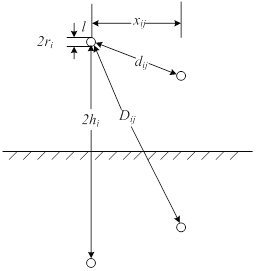
\includegraphics{导体镜像截面图.png}
\caption{导体镜像截面图}
\end{figure}

    \begin{Verbatim}[commandchars=\\\{\}]
{\color{incolor}In [{\color{incolor}63}]:} \PY{k}{def} \PY{n+nf}{calc\PYZus{}potential\PYZus{}coefficient}\PY{p}{(}\PY{n}{c\PYZus{}xy}\PY{p}{,}\PY{n}{r}\PY{p}{)}\PY{p}{:}
             \PY{l+s+sd}{\PYZdq{}\PYZdq{}\PYZdq{} }
         \PY{l+s+sd}{    计算电位系数矩阵P}
         \PY{l+s+sd}{    c\PYZus{}xy=conductors\PYZus{}coordinate  \PYZsh{} 多导体坐标数组 (x,y),单位 m}
         \PY{l+s+sd}{    r=conductors\PYZus{}calc\PYZus{}radius    \PYZsh{} 多导体计算半径,单位 m}
         \PY{l+s+sd}{    \PYZdq{}\PYZdq{}\PYZdq{}}    
             \PY{n}{n}\PY{o}{=}\PY{n}{np}\PY{o}{.}\PY{n}{shape}\PY{p}{(}\PY{n}{c\PYZus{}xy}\PY{p}{)}\PY{p}{[}\PY{l+m+mi}{1}\PY{p}{]}
             \PY{n}{P}\PY{o}{=}\PY{n}{np}\PY{o}{.}\PY{n}{empty}\PY{p}{(}\PY{p}{(}\PY{n}{n}\PY{p}{,}\PY{n}{n}\PY{p}{)}\PY{p}{,}\PY{n}{np}\PY{o}{.}\PY{n}{float64}\PY{p}{)}
             \PY{k}{for} \PY{n}{i} \PY{o+ow}{in} \PY{n+nb}{range}\PY{p}{(}\PY{n}{n}\PY{p}{)}\PY{p}{:}
                 \PY{k}{for} \PY{n}{j} \PY{o+ow}{in} \PY{n+nb}{range}\PY{p}{(}\PY{n}{n}\PY{p}{)}\PY{p}{:}
                     \PY{k}{if} \PY{n}{i}\PY{o}{==}\PY{n}{j}\PY{p}{:}
                         \PY{n}{P}\PY{p}{[}\PY{n}{i}\PY{p}{,}\PY{n}{j}\PY{p}{]}\PY{o}{=}\PY{l+m+mi}{18}\PY{o}{*}\PY{l+m+mi}{10}\PY{o}{*}\PY{o}{*}\PY{o}{+}\PY{l+m+mi}{9}\PY{o}{*}\PY{n}{np}\PY{o}{.}\PY{n}{log}\PY{p}{(}\PY{l+m+mi}{2}\PY{o}{*}\PY{n}{c\PYZus{}xy}\PY{p}{[}\PY{l+m+mi}{1}\PY{p}{,}\PY{n}{i}\PY{p}{]}\PY{o}{/}\PY{n}{r}\PY{p}{[}\PY{n}{i}\PY{p}{]}\PY{p}{)}\PY{c+c1}{\PYZsh{}调用y轴坐标}
                     \PY{k}{else}\PY{p}{:}
                         \PY{n}{Dij}\PY{o}{=}\PY{n}{np}\PY{o}{.}\PY{n}{sqrt}\PY{p}{(}\PY{p}{(}\PY{n}{c\PYZus{}xy}\PY{p}{[}\PY{l+m+mi}{0}\PY{p}{,}\PY{n}{i}\PY{p}{]}\PY{o}{\PYZhy{}}\PY{n}{c\PYZus{}xy}\PY{p}{[}\PY{l+m+mi}{0}\PY{p}{,}\PY{n}{j}\PY{p}{]}\PY{p}{)}\PY{o}{*}\PY{o}{*}\PY{l+m+mi}{2}\PY{o}{+}\PY{p}{(}\PY{n}{c\PYZus{}xy}\PY{p}{[}\PY{l+m+mi}{1}\PY{p}{,}\PY{n}{i}\PY{p}{]}\PY{o}{+}\PY{n}{c\PYZus{}xy}\PY{p}{[}\PY{l+m+mi}{1}\PY{p}{,}\PY{n}{j}\PY{p}{]}\PY{p}{)}\PY{o}{*}\PY{o}{*}\PY{l+m+mi}{2}\PY{p}{)}
                         \PY{c+c1}{\PYZsh{} 导线i与导线j的镜像之间的距离,单位m}
                         \PY{n}{dij}\PY{o}{=}\PY{n}{np}\PY{o}{.}\PY{n}{sqrt}\PY{p}{(}\PY{p}{(}\PY{n}{c\PYZus{}xy}\PY{p}{[}\PY{l+m+mi}{0}\PY{p}{,}\PY{n}{i}\PY{p}{]}\PY{o}{\PYZhy{}}\PY{n}{c\PYZus{}xy}\PY{p}{[}\PY{l+m+mi}{0}\PY{p}{,}\PY{n}{j}\PY{p}{]}\PY{p}{)}\PY{o}{*}\PY{o}{*}\PY{l+m+mi}{2}\PY{o}{+}\PY{p}{(}\PY{n}{c\PYZus{}xy}\PY{p}{[}\PY{l+m+mi}{1}\PY{p}{,}\PY{n}{i}\PY{p}{]}\PY{o}{\PYZhy{}}\PY{n}{c\PYZus{}xy}\PY{p}{[}\PY{l+m+mi}{1}\PY{p}{,}\PY{n}{j}\PY{p}{]}\PY{p}{)}\PY{o}{*}\PY{o}{*}\PY{l+m+mi}{2}\PY{p}{)}
                         \PY{c+c1}{\PYZsh{} 导线i与导线j之间的距离,单位m}
                         \PY{n}{P}\PY{p}{[}\PY{n}{i}\PY{p}{,}\PY{n}{j}\PY{p}{]}\PY{o}{=}\PY{l+m+mi}{18}\PY{o}{*}\PY{l+m+mi}{10}\PY{o}{*}\PY{o}{*}\PY{o}{+}\PY{l+m+mi}{9}\PY{o}{*}\PY{n}{np}\PY{o}{.}\PY{n}{log}\PY{p}{(}\PY{n}{Dij}\PY{o}{/}\PY{n}{dij}\PY{p}{)}
             \PY{k}{return} \PY{n}{P}
\end{Verbatim}


    \begin{Verbatim}[commandchars=\\\{\}]
{\color{incolor}In [{\color{incolor}64}]:} \PY{n}{c\PYZus{}xy}\PY{o}{=}\PY{n}{conductors\PYZus{}coordinate}
         \PY{n}{r}\PY{o}{=}\PY{n}{conductors\PYZus{}calc\PYZus{}radius}
         \PY{n}{calc\PYZus{}potential\PYZus{}coefficient}\PY{p}{(}\PY{n}{c\PYZus{}xy}\PY{p}{,}\PY{n}{r}\PY{p}{)}\PY{c+c1}{\PYZsh{} 调用函数 得14*14的电位系数矩阵P}
\end{Verbatim}


\begin{Verbatim}[commandchars=\\\{\}]
{\color{outcolor}Out[{\color{outcolor}64}]:} array([[1.3800e+11, 4.3962e+10, 2.0588e+10, 5.6780e+09, 5.6780e+09, 2.3569e+10, 1.9196e+09, 1.7953e+10, 1.8880e+10, 1.0741e+10, 3.9241e+09, 3.1031e+09, 1.1586e+10, 8.8458e+08],
                [4.3962e+10, 1.3806e+11, 2.3441e+10, 4.7789e+09, 4.7789e+09, 2.6579e+10, 1.7854e+09, 1.8880e+10, 2.0723e+10, 1.2141e+10, 3.6357e+09, 3.0156e+09, 1.2988e+10, 9.3277e+08],
                [2.0588e+10, 2.3441e+10, 1.3481e+11, 3.5827e+09, 3.0956e+09, 5.1530e+10, 2.1201e+09, 1.0741e+10, 1.2141e+10, 8.3095e+09, 2.0769e+09, 1.7404e+09, 8.6241e+09, 5.8208e+08],
                [5.6780e+09, 4.7789e+09, 3.5827e+09, 5.2355e+10, 9.1185e+09, 4.0049e+09, 1.2403e+09, 3.1031e+09, 3.0156e+09, 1.7404e+09, 1.3358e+09, 8.1172e+08, 1.8953e+09, 1.7246e+08],
                [5.6780e+09, 4.7789e+09, 3.0956e+09, 9.1185e+09, 5.2355e+10, 3.4724e+09, 6.4720e+08, 3.9241e+09, 3.6357e+09, 2.0769e+09, 2.5558e+09, 1.3358e+09, 2.2881e+09, 2.3690e+08],
                [2.3569e+10, 2.6579e+10, 5.1530e+10, 4.0049e+09, 3.4724e+09, 1.3774e+11, 2.2305e+09, 1.1586e+10, 1.2988e+10, 8.6241e+09, 2.2881e+09, 1.8953e+09, 9.0056e+09, 6.1761e+08],
                [1.9196e+09, 1.7854e+09, 2.1201e+09, 1.2403e+09, 6.4720e+08, 2.2305e+09, 9.4152e+10, 8.8458e+08, 9.3277e+08, 5.8208e+08, 2.3690e+08, 1.7246e+08, 6.1761e+08, 4.7135e+07],
                [1.7953e+10, 1.8880e+10, 1.0741e+10, 3.1031e+09, 3.9241e+09, 1.1586e+10, 8.8458e+08, 1.3800e+11, 4.3962e+10, 2.0588e+10, 5.6780e+09, 5.6780e+09, 2.3569e+10, 1.9196e+09],
                [1.8880e+10, 2.0723e+10, 1.2141e+10, 3.0156e+09, 3.6357e+09, 1.2988e+10, 9.3277e+08, 4.3962e+10, 1.3806e+11, 2.3441e+10, 4.7789e+09, 4.7789e+09, 2.6579e+10, 1.7854e+09],
                [1.0741e+10, 1.2141e+10, 8.3095e+09, 1.7404e+09, 2.0769e+09, 8.6241e+09, 5.8208e+08, 2.0588e+10, 2.3441e+10, 1.3481e+11, 3.0956e+09, 3.5827e+09, 5.1530e+10, 2.1201e+09],
                [3.9241e+09, 3.6357e+09, 2.0769e+09, 1.3358e+09, 2.5558e+09, 2.2881e+09, 2.3690e+08, 5.6780e+09, 4.7789e+09, 3.0956e+09, 5.2355e+10, 9.1185e+09, 3.4724e+09, 6.4720e+08],
                [3.1031e+09, 3.0156e+09, 1.7404e+09, 8.1172e+08, 1.3358e+09, 1.8953e+09, 1.7246e+08, 5.6780e+09, 4.7789e+09, 3.5827e+09, 9.1185e+09, 5.2355e+10, 4.0049e+09, 1.2403e+09],
                [1.1586e+10, 1.2988e+10, 8.6241e+09, 1.8953e+09, 2.2881e+09, 9.0056e+09, 6.1761e+08, 2.3569e+10, 2.6579e+10, 5.1530e+10, 3.4724e+09, 4.0049e+09, 1.3774e+11, 2.2305e+09],
                [8.8458e+08, 9.3277e+08, 5.8208e+08, 1.7246e+08, 2.3690e+08, 6.1761e+08, 4.7135e+07, 1.9196e+09, 1.7854e+09, 2.1201e+09, 6.4720e+08, 1.2403e+09, 2.2305e+09, 9.4152e+10]])
\end{Verbatim}
            
    \subsection{导线合并}\label{ux5bfcux7ebfux5408ux5e76}

    ** 函数名: merge\_potential\_coefficient(P,m,k)** * parameters:\\
1. P: n×n 维数组,电位系数 ;\\
2. m: 第 m 号导线(导线序号从0开始); 3. k: 第 k 号导线,m<k≤n, *
Return: 1. P: n-1×n-1 维数组,归并后的电位系数

\begin{itemize}
\tightlist
\item
  功能: 导线k并入导线m,计算修正后的电位系数P
\end{itemize}

导线k并入m公式推导:

\begin{equation} 
 \begin{bmatrix}
  u_1\\
  \vdots\\
  u_m\\
  \vdots\\
  u_k\\
  \vdots\\
  u_n
  \end{bmatrix} =
  \begin{bmatrix}
  P_{11}&\dots& P_{1m}&\dots&P_{1k}&\dots&P_{1n}\\
  \vdots& &\vdots& &\vdots& &\vdots\\
  P_{m1}&\dots& P_{mm}&\dots&P_{mk}&\dots&P_{mn}\\
   \vdots& &\vdots& &\vdots& &\vdots\\
    P_{k1}&\dots& P_{km}&\dots&P_{kk}&\dots&P_{kn}\\
   \vdots& &\vdots& &\vdots& &\vdots\\ 
    P_{n1}&\dots& P_{nm}&\dots&P_{nk}&\dots&P_{nn}\\
   \end{bmatrix}
   \begin{bmatrix}
   q_1\\
   \vdots\\
  q_m\\
  \vdots\\
  q_k\\
  \vdots\\
  q_n
 \end{bmatrix}
 \end{equation}

令 \(q_{m}=q_{m}+q_{k}\) 有:

\begin{equation} 
 \begin{bmatrix}
  u_1\\
  \vdots\\
  u_m\\
  \vdots\\
  u_k\\
  \vdots\\
  u_n
  \end{bmatrix} =
  \begin{bmatrix}
  P_{11}&\dots& P_{1m}&\dots&(P_{1k}-P_{1m})&\dots&P_{1n}\\
  \vdots& &\vdots& &\vdots& &\vdots\\
  P_{m1}&\dots& P_{mm}&\dots&(P_{mk}-P_{mm})&\dots&P_{mn}\\
  \vdots& &\vdots& &\vdots& &\vdots\\
   P_{k1}&\dots& P_{km}&\dots&(P_{kk}-P_{km})&\dots&P_{kn}\\
  \vdots& &\vdots& &\vdots& &\vdots\\ 
   P_{n1}&\dots& P_{nm}&\dots&(P_{nk}-P_{nm})&\dots&P_{nn}\\
  \end{bmatrix}
  \begin{bmatrix}
   q_1\\
   \vdots\\
  q_m+q_k\\
  \vdots\\
  q_k\\
  \vdots\\
  q_n
 \end{bmatrix}
\end{equation}

P矩阵第k列参数发生变化,修正公式为:\[P_{ik}=P_{ik}-P_{im} ( i=0,1,...,n), q_m=q_m+q_k\].

方程中,\(u_{k}-u_{m}=0\),得方程

\begin{equation*} 
 \begin{bmatrix}
  u_1\\
  \vdots\\
  u_m\\
  \vdots\\
  0\\
  \vdots\\
  u_n
  \end{bmatrix} =
  \begin{bmatrix}
  P_{11}&\dots& P_{1m}&\dots&P_{1k}&\dots&P_{1n}\\
  \vdots& &\vdots& &\vdots& &\vdots\\
  P_{m1}&\dots& P_{mm}&\dots&P_{mk}&\dots&P_{mn}\\
   \vdots& &\vdots& &\vdots& &\vdots\\
    P_{k1}- P_{m1}&\dots& P_{km}-P_{mm}&\dots&P_{kk}-P_{mk}&\dots&P_{kn}-P_{mn}\\
   \vdots& &\vdots& &\vdots& &\vdots\\ 
    P_{n1}&\dots& P_{nm}&\dots&P_{nk}&\dots&P_{nn}\\
   \end{bmatrix}
   \begin{bmatrix}
   q_1\\
   \vdots\\
  q_m\\
  \vdots\\
  q_k\\
  \vdots\\
  q_n
 \end{bmatrix}
\end{equation*}

第k行等式有:
\[ 0= (P_{k1}- P_{m1})q_1+\dots+(P_{km}-P_{mm})q_m+\dots+(P_{kk}-P_{mk})q_k+\dots+(P_{kn}-P_{mn})q_n\]

可以求得:
\[q_k=-\frac{(P_{k1}- P_{m1})}{(P_{kk}-P_{mk})}q_1-\dots-\frac{(P_{km}- P_{mm})}{(P_{kk}-P_{mk})}q_m\dots-\frac{(P_{kn}- P_{mn})}{(P_{kk}-P_{mk})}q_n\]

令\(K_j=\frac{P_{kj}- P_{mj}}{P_{kk}-P_{mk}}\) (j≠k),有
\[q_k=-K_1q_1-\dots-K_m q_m-\dots-K_n q_n\]

导线电压\(u_i\)写成方程有:
\[u_i=P_{i1}q_1+\dots+P_{im}q_m+\dots+P_{ik}q_k+\dots+P_{in}q_n\]

把\(q_k\)代入方程中,得到
\[u_i=(P_{i1}-P_{ik}K_1)q_1+\dots+(P_{im}-P_{ik}K_m)q_m+\dots+(P_{in}-P_{ik}K_n)q_n\]

取(i,j=0,1,...,n; i≠k;j≠k),可以得到合并矩阵元素\(P_{ij}\).
\[P_{ij}=P_{ij}-P_{ik}K_j=P_{ij}-P_{ik}\frac{P_{kj}- P_{mj}}{P_{kk}-P_{mk}}\]

总之,导线k合并到导线m,P参数的修正步骤归纳如下:

(1)\(P_{ik}=P_{ik}-P_{im}\) ( i=0,1,...,n)

(2)\(P_{ij}=P_{ij}-P_{ik}K_j=P_{ij}-P_{ik}\frac{P_{kj}- P_{mj}}{P_{kk}-P_{mk}}\)
(i,j=0,1,...,n; i≠k;j≠k)

(3)除P中的第k行第k列,P降n-1阶,为合并后n-1根导线的电位系数矩阵。

    \begin{Verbatim}[commandchars=\\\{\}]
{\color{incolor}In [{\color{incolor}65}]:} \PY{k}{def} \PY{n+nf}{merge\PYZus{}potential\PYZus{}coefficient}\PY{p}{(}\PY{n}{P}\PY{p}{,}\PY{n}{m}\PY{p}{,}\PY{n}{k}\PY{p}{)}\PY{p}{:}
             \PY{l+s+sd}{\PYZsq{}\PYZsq{}\PYZsq{}}
         \PY{l+s+sd}{    P:矩阵(电位系数矩阵)}
         \PY{l+s+sd}{    m:要合并的导线之一}
         \PY{l+s+sd}{    k:要合并的导线之二,(最终被消去,合并到m上,且m\PYZlt{}k)}
         \PY{l+s+sd}{    \PYZsq{}\PYZsq{}\PYZsq{}}
             \PY{n}{n}\PY{o}{=}\PY{n}{np}\PY{o}{.}\PY{n}{shape}\PY{p}{(}\PY{n}{P}\PY{p}{)}\PY{p}{[}\PY{l+m+mi}{0}\PY{p}{]}
             \PY{k}{for} \PY{n}{i} \PY{o+ow}{in} \PY{n+nb}{range}\PY{p}{(}\PY{n}{n}\PY{p}{)}\PY{p}{:}
                 \PY{n}{P}\PY{p}{[}\PY{n}{i}\PY{p}{,}\PY{n}{k}\PY{p}{]}\PY{o}{=}\PY{n}{P}\PY{p}{[}\PY{n}{i}\PY{p}{,}\PY{n}{k}\PY{p}{]}\PY{o}{\PYZhy{}}\PY{n}{P}\PY{p}{[}\PY{n}{i}\PY{p}{,}\PY{n}{m}\PY{p}{]}
                  
             \PY{k}{for} \PY{n}{i} \PY{o+ow}{in} \PY{n+nb}{range}\PY{p}{(}\PY{n}{n}\PY{p}{)}\PY{p}{:}
                 \PY{k}{for} \PY{n}{j} \PY{o+ow}{in} \PY{n+nb}{range}\PY{p}{(}\PY{n}{n}\PY{p}{)}\PY{p}{:}
                     \PY{k}{if} \PY{n}{i}\PY{o}{!=}\PY{n}{k} \PY{o+ow}{or} \PY{n}{j}\PY{o}{!=}\PY{n}{k}\PY{p}{:}
                         \PY{n}{P}\PY{p}{[}\PY{n}{i}\PY{p}{,}\PY{n}{j}\PY{p}{]}\PY{o}{=}\PY{n}{P}\PY{p}{[}\PY{n}{i}\PY{p}{,}\PY{n}{j}\PY{p}{]}\PY{o}{\PYZhy{}}\PY{p}{(}\PY{p}{(}\PY{n}{P}\PY{p}{[}\PY{n}{k}\PY{p}{,}\PY{n}{j}\PY{p}{]}\PY{o}{\PYZhy{}}\PY{n}{P}\PY{p}{[}\PY{n}{m}\PY{p}{,}\PY{n}{j}\PY{p}{]}\PY{p}{)}\PY{o}{/}\PY{p}{(}\PY{n}{P}\PY{p}{[}\PY{n}{k}\PY{p}{,}\PY{n}{k}\PY{p}{]}\PY{o}{\PYZhy{}}\PY{n}{P}\PY{p}{[}\PY{n}{m}\PY{p}{,}\PY{n}{k}\PY{p}{]}\PY{p}{)}\PY{p}{)}\PY{o}{*}\PY{n}{P}\PY{p}{[}\PY{n}{i}\PY{p}{,}\PY{n}{k}\PY{p}{]}
                                 
                   
             \PY{n}{E}\PY{o}{=}\PY{n}{np}\PY{o}{.}\PY{n}{empty}\PY{p}{(}\PY{p}{(}\PY{n}{n}\PY{o}{\PYZhy{}}\PY{l+m+mi}{1}\PY{p}{,}\PY{n}{n}\PY{o}{\PYZhy{}}\PY{l+m+mi}{1}\PY{p}{)}\PY{p}{,}\PY{n}{np}\PY{o}{.}\PY{n}{float64}\PY{p}{)}
             \PY{k}{for} \PY{n}{i} \PY{o+ow}{in} \PY{n+nb}{range}\PY{p}{(}\PY{n}{n}\PY{p}{)}\PY{p}{:}
                 \PY{k}{for} \PY{n}{j} \PY{o+ow}{in} \PY{n+nb}{range}\PY{p}{(}\PY{n}{n}\PY{p}{)}\PY{p}{:}
                     \PY{k}{if} \PY{n}{i}\PY{o}{\PYZlt{}}\PY{n}{k}\PY{p}{:}
                         \PY{k}{if} \PY{n}{j}\PY{o}{\PYZlt{}}\PY{n}{k}\PY{p}{:}
                             \PY{n}{E}\PY{p}{[}\PY{n}{i}\PY{p}{,}\PY{n}{j}\PY{p}{]}\PY{o}{=}\PY{n}{P}\PY{p}{[}\PY{n}{i}\PY{p}{,}\PY{n}{j}\PY{p}{]}
                         \PY{k}{if} \PY{n}{j}\PY{o}{\PYZgt{}}\PY{n}{k}\PY{p}{:}
                             \PY{n}{E}\PY{p}{[}\PY{n}{i}\PY{p}{,}\PY{n}{j}\PY{o}{\PYZhy{}}\PY{l+m+mi}{1}\PY{p}{]}\PY{o}{=}\PY{n}{P}\PY{p}{[}\PY{n}{i}\PY{p}{,}\PY{n}{j}\PY{p}{]}
                     \PY{k}{if} \PY{n}{i}\PY{o}{\PYZgt{}}\PY{n}{k}\PY{p}{:}
                         \PY{k}{if} \PY{n}{j}\PY{o}{\PYZlt{}}\PY{n}{k}\PY{p}{:}
                             \PY{n}{E}\PY{p}{[}\PY{n}{i}\PY{o}{\PYZhy{}}\PY{l+m+mi}{1}\PY{p}{,}\PY{n}{j}\PY{p}{]}\PY{o}{=}\PY{n}{P}\PY{p}{[}\PY{n}{i}\PY{p}{,}\PY{n}{j}\PY{p}{]}
                         \PY{k}{if} \PY{n}{j}\PY{o}{\PYZgt{}}\PY{n}{k}\PY{p}{:}
                             \PY{n}{E}\PY{p}{[}\PY{n}{i}\PY{o}{\PYZhy{}}\PY{l+m+mi}{1}\PY{p}{,}\PY{n}{j}\PY{o}{\PYZhy{}}\PY{l+m+mi}{1}\PY{p}{]}\PY{o}{=}\PY{n}{P}\PY{p}{[}\PY{n}{i}\PY{p}{,}\PY{n}{j}\PY{p}{]}
             
             \PY{k}{return} \PY{n}{E}
\end{Verbatim}


    \begin{Verbatim}[commandchars=\\\{\}]
{\color{incolor}In [{\color{incolor}66}]:} \PY{k}{def} \PY{n+nf}{combine\PYZus{}line}\PY{p}{(}\PY{n}{str1}\PY{p}{,}\PY{n}{str2}\PY{p}{,}\PY{n}{P}\PY{p}{,}\PY{n}{Line\PYZus{}name}\PY{p}{)}\PY{p}{:}
             \PY{l+s+sd}{\PYZsq{}\PYZsq{}\PYZsq{}}
         \PY{l+s+sd}{    str1:要合并的导线之一的名称}
         \PY{l+s+sd}{    str2:要合并的导线之二的名称,(最终被消去,合并到str1上)}
         \PY{l+s+sd}{    P:矩阵(电位系数矩阵)(需要合并的矩阵)}
         \PY{l+s+sd}{    Line\PYZus{}name:与矩阵P匹配的导线名称列表}
         \PY{l+s+sd}{    输出合并后的矩阵P‘}
         \PY{l+s+sd}{    \PYZsq{}\PYZsq{}\PYZsq{}}
         \PY{c+c1}{\PYZsh{}     print(\PYZsq{}combine\PYZus{}line1:\PYZbs{}n\PYZsq{},P)}
             \PY{n}{m} \PY{o}{=} \PY{n}{Line\PYZus{}name}\PY{o}{.}\PY{n}{index}\PY{p}{(}\PY{n}{str1}\PY{p}{)}
             \PY{n}{k} \PY{o}{=} \PY{n}{Line\PYZus{}name}\PY{o}{.}\PY{n}{index}\PY{p}{(}\PY{n}{str2}\PY{p}{)}
             \PY{k}{if} \PY{n}{str1} \PY{o+ow}{not} \PY{o+ow}{in} \PY{n}{Line\PYZus{}name}\PY{p}{:}
                 \PY{n+nb}{print}\PY{p}{(}\PY{l+s+s1}{\PYZsq{}}\PY{l+s+s1}{没有}\PY{l+s+s1}{\PYZsq{}}\PY{o}{+}\PY{n}{str1}\PY{o}{+}\PY{l+s+s1}{\PYZsq{}}\PY{l+s+s1}{线或此线已经合并}\PY{l+s+s1}{\PYZsq{}}\PY{p}{)}
             \PY{k}{elif} \PY{n}{str2} \PY{o+ow}{not} \PY{o+ow}{in} \PY{n}{Line\PYZus{}name}\PY{p}{:}
                 \PY{n+nb}{print}\PY{p}{(}\PY{l+s+s1}{\PYZsq{}}\PY{l+s+s1}{没有}\PY{l+s+s1}{\PYZsq{}}\PY{o}{+}\PY{n}{str2}\PY{o}{+}\PY{l+s+s1}{\PYZsq{}}\PY{l+s+s1}{线或此线已经合并}\PY{l+s+s1}{\PYZsq{}}\PY{p}{)}
             \PY{k}{elif} \PY{n}{m} \PY{o}{\PYZgt{}}\PY{o}{=} \PY{n}{k}\PY{p}{:}
                 \PY{n+nb}{print}\PY{p}{(}\PY{l+s+s1}{\PYZsq{}}\PY{l+s+s1}{不满足m\PYZlt{}k}\PY{l+s+s1}{\PYZsq{}}\PY{p}{)}
             \PY{k}{else}\PY{p}{:}
                 \PY{n+nb}{print}\PY{p}{(}\PY{l+s+s1}{\PYZsq{}}\PY{l+s+s1}{合并}\PY{l+s+s1}{\PYZsq{}}\PY{p}{,}\PY{n}{str1}\PY{o}{+}\PY{l+s+s1}{\PYZsq{}}\PY{l+s+s1}{与}\PY{l+s+s1}{\PYZsq{}}\PY{o}{+}\PY{n}{str2}\PY{p}{)}
                 \PY{n}{a} \PY{o}{=} \PY{n}{Line\PYZus{}name}\PY{o}{.}\PY{n}{index}\PY{p}{(}\PY{n}{str1}\PY{p}{)}
                 \PY{n}{b} \PY{o}{=} \PY{n}{Line\PYZus{}name}\PY{o}{.}\PY{n}{index}\PY{p}{(}\PY{n}{str2}\PY{p}{)}
                 \PY{n}{P}\PY{o}{=}\PY{n}{merge\PYZus{}potential\PYZus{}coefficient}\PY{p}{(}\PY{n}{P}\PY{p}{,}\PY{n}{m}\PY{p}{,}\PY{n}{k}\PY{p}{)}\PY{c+c1}{\PYZsh{}接触导线1与承力索1合并}
         \PY{c+c1}{\PYZsh{}         print(\PYZsq{}combine\PYZus{}line2:\PYZbs{}n\PYZsq{},P)}
                 \PY{n}{Line\PYZus{}name}\PY{o}{.}\PY{n}{remove}\PY{p}{(}\PY{n}{Line\PYZus{}name}\PY{p}{[}\PY{n}{b}\PY{p}{]}\PY{p}{)}
                 \PY{n+nb}{print}\PY{p}{(}\PY{l+s+s1}{\PYZsq{}}\PY{l+s+s1}{m:}\PY{l+s+s1}{\PYZsq{}}\PY{p}{,}\PY{n}{m}\PY{p}{,}\PY{l+s+s1}{\PYZsq{}}\PY{l+s+s1}{k:}\PY{l+s+s1}{\PYZsq{}}\PY{p}{,}\PY{n}{k}\PY{p}{)}
                 \PY{k}{return} \PY{n}{P}\PY{p}{,}\PY{n}{Line\PYZus{}name}
\end{Verbatim}


    AT牵引网络由14根导线逐步合并成6根导线:

(1) 1. 接触线(CW1)+ 2.承力索(MW1)

(2) 3.正馈线(PF1)

(3) 4.钢轨1(RA1)+5.钢轨2(RA2)+6.保护线(PW1)+7.综合地线(E1)

(4) 8. 接触线(CW2)+ 9.承力索(MW2)

(5) 10.正馈线(PF2)

(6) 11.钢轨3(RA3)+12.钢轨4(RA4)+13.保护线(PW2)+14.综合地线(E2)

    \begin{Verbatim}[commandchars=\\\{\}]
{\color{incolor}In [{\color{incolor}67}]:} \PY{n}{c\PYZus{}xy}\PY{o}{=}\PY{n}{conductors\PYZus{}coordinate}
         \PY{n}{r}\PY{o}{=}\PY{n}{conductors\PYZus{}calc\PYZus{}radius}
         \PY{n}{P}\PY{o}{=}\PY{n}{calc\PYZus{}potential\PYZus{}coefficient}\PY{p}{(}\PY{n}{c\PYZus{}xy}\PY{p}{,}\PY{n}{r}\PY{p}{)}
         \PY{n}{line\PYZus{}name}\PY{o}{=}\PY{n}{para}\PY{p}{[}\PY{l+s+s1}{\PYZsq{}}\PY{l+s+s1}{名称}\PY{l+s+s1}{\PYZsq{}}\PY{p}{]}
         \PY{n}{Line\PYZus{}name}\PY{o}{=}\PY{n+nb}{list}\PY{p}{(}\PY{n}{line\PYZus{}name}\PY{p}{)}
         \PY{n}{P}\PY{p}{,}\PY{n}{Line\PYZus{}name} \PY{o}{=} \PY{n}{combine\PYZus{}line}\PY{p}{(}\PY{l+s+s1}{\PYZsq{}}\PY{l+s+s1}{接触导线1}\PY{l+s+s1}{\PYZsq{}}\PY{p}{,}\PY{l+s+s1}{\PYZsq{}}\PY{l+s+s1}{承力索1}\PY{l+s+s1}{\PYZsq{}}\PY{p}{,}\PY{n}{P}\PY{p}{,}\PY{n}{Line\PYZus{}name}\PY{p}{)}\PY{c+c1}{\PYZsh{} 线1}
         \PY{n}{P}\PY{p}{,}\PY{n}{Line\PYZus{}name} \PY{o}{=} \PY{n}{combine\PYZus{}line}\PY{p}{(}\PY{l+s+s1}{\PYZsq{}}\PY{l+s+s1}{接触导线2}\PY{l+s+s1}{\PYZsq{}}\PY{p}{,}\PY{l+s+s1}{\PYZsq{}}\PY{l+s+s1}{承力索2}\PY{l+s+s1}{\PYZsq{}}\PY{p}{,}\PY{n}{P}\PY{p}{,}\PY{n}{Line\PYZus{}name}\PY{p}{)}\PY{c+c1}{\PYZsh{} 线1\PYZhy{}1}
         
         \PY{n}{P}\PY{p}{,}\PY{n}{Line\PYZus{}name} \PY{o}{=} \PY{n}{combine\PYZus{}line}\PY{p}{(}\PY{l+s+s1}{\PYZsq{}}\PY{l+s+s1}{钢轨1}\PY{l+s+s1}{\PYZsq{}}\PY{p}{,}\PY{l+s+s1}{\PYZsq{}}\PY{l+s+s1}{钢轨2}\PY{l+s+s1}{\PYZsq{}}\PY{p}{,}\PY{n}{P}\PY{p}{,}\PY{n}{Line\PYZus{}name}\PY{p}{)}
         \PY{n}{P}\PY{p}{,}\PY{n}{Line\PYZus{}name} \PY{o}{=} \PY{n}{combine\PYZus{}line}\PY{p}{(}\PY{l+s+s1}{\PYZsq{}}\PY{l+s+s1}{钢轨1}\PY{l+s+s1}{\PYZsq{}}\PY{p}{,}\PY{l+s+s1}{\PYZsq{}}\PY{l+s+s1}{保护线1}\PY{l+s+s1}{\PYZsq{}}\PY{p}{,}\PY{n}{P}\PY{p}{,}\PY{n}{Line\PYZus{}name}\PY{p}{)}
         \PY{n}{P}\PY{p}{,}\PY{n}{Line\PYZus{}name} \PY{o}{=} \PY{n}{combine\PYZus{}line}\PY{p}{(}\PY{l+s+s1}{\PYZsq{}}\PY{l+s+s1}{钢轨1}\PY{l+s+s1}{\PYZsq{}}\PY{p}{,}\PY{l+s+s1}{\PYZsq{}}\PY{l+s+s1}{综合地线1}\PY{l+s+s1}{\PYZsq{}}\PY{p}{,}\PY{n}{P}\PY{p}{,}\PY{n}{Line\PYZus{}name}\PY{p}{)}\PY{c+c1}{\PYZsh{} 线2}
         
         \PY{n}{P}\PY{p}{,}\PY{n}{Line\PYZus{}name} \PY{o}{=} \PY{n}{combine\PYZus{}line}\PY{p}{(}\PY{l+s+s1}{\PYZsq{}}\PY{l+s+s1}{钢轨3}\PY{l+s+s1}{\PYZsq{}}\PY{p}{,}\PY{l+s+s1}{\PYZsq{}}\PY{l+s+s1}{钢轨4}\PY{l+s+s1}{\PYZsq{}}\PY{p}{,}\PY{n}{P}\PY{p}{,}\PY{n}{Line\PYZus{}name}\PY{p}{)}
         \PY{n}{P}\PY{p}{,}\PY{n}{Line\PYZus{}name} \PY{o}{=} \PY{n}{combine\PYZus{}line}\PY{p}{(}\PY{l+s+s1}{\PYZsq{}}\PY{l+s+s1}{钢轨3}\PY{l+s+s1}{\PYZsq{}}\PY{p}{,}\PY{l+s+s1}{\PYZsq{}}\PY{l+s+s1}{保护线2}\PY{l+s+s1}{\PYZsq{}}\PY{p}{,}\PY{n}{P}\PY{p}{,}\PY{n}{Line\PYZus{}name}\PY{p}{)}
         \PY{n}{P}\PY{p}{,}\PY{n}{Line\PYZus{}name} \PY{o}{=} \PY{n}{combine\PYZus{}line}\PY{p}{(}\PY{l+s+s1}{\PYZsq{}}\PY{l+s+s1}{钢轨3}\PY{l+s+s1}{\PYZsq{}}\PY{p}{,}\PY{l+s+s1}{\PYZsq{}}\PY{l+s+s1}{综合地线2}\PY{l+s+s1}{\PYZsq{}}\PY{p}{,}\PY{n}{P}\PY{p}{,}\PY{n}{Line\PYZus{}name}\PY{p}{)}\PY{c+c1}{\PYZsh{} 线2\PYZhy{}2}
         
         \PY{n+nb}{print}\PY{p}{(}\PY{n}{P}\PY{o}{.}\PY{n}{shape}\PY{p}{,}\PY{n}{Line\PYZus{}name}\PY{p}{)}    
         \PY{n}{np}\PY{o}{.}\PY{n}{set\PYZus{}printoptions}\PY{p}{(}\PY{n}{precision}\PY{o}{=}\PY{l+m+mi}{3}\PY{p}{,}\PY{n}{linewidth}\PY{o}{=}\PY{l+m+mi}{214}\PY{p}{,}\PY{n}{suppress}\PY{o}{=}\PY{k+kc}{True}\PY{p}{)}
         \PY{n+nb}{print}\PY{p}{(}\PY{l+s+s1}{\PYZsq{}}\PY{l+s+s1}{P矩阵 e+10 : }\PY{l+s+se}{\PYZbs{}n}\PY{l+s+s1}{ }\PY{l+s+si}{\PYZob{}\PYZcb{}}\PY{l+s+s1}{\PYZsq{}}\PY{o}{.}\PY{n}{format}\PY{p}{(}\PY{n}{P}\PY{o}{*}\PY{l+m+mi}{10}\PY{o}{*}\PY{o}{*}\PY{o}{\PYZhy{}}\PY{l+m+mi}{10}\PY{p}{)}\PY{p}{)}
\end{Verbatim}


    \begin{Verbatim}[commandchars=\\\{\}]
合并 接触导线1与承力索1
m: 0 k: 1
合并 接触导线2与承力索2
m: 6 k: 7
合并 钢轨1与钢轨2
m: 2 k: 3
合并 钢轨1与保护线1
m: 2 k: 3
合并 钢轨1与综合地线1
m: 2 k: 3
合并 钢轨3与钢轨4
m: 5 k: 6
合并 钢轨3与保护线2
m: 5 k: 6
合并 钢轨3与综合地线2
m: 5 k: 6
(6, 6) ['接触导线1', '正馈线1', '钢轨1', '接触导线2', '正馈线2', '钢轨3']
P矩阵 e+10 : 
 [[ 8.807  1.426  0.715  1.729  0.802  0.402]
 [ 1.426 11.928  0.935  1.056  0.611  0.252]
 [ 0.715  0.935  2.095  0.291  0.142  0.099]
 [ 1.729  1.056  0.291  8.863  1.472  0.725]
 [ 0.802  0.611  0.142  1.472 11.97   0.947]
 [ 0.402  0.252  0.099  0.725  0.947  2.068]]

    \end{Verbatim}

    \subsection{电容系数矩阵计算}\label{ux7535ux5bb9ux7cfbux6570ux77e9ux9635ux8ba1ux7b97}

    \begin{Verbatim}[commandchars=\\\{\}]
{\color{incolor}In [{\color{incolor}68}]:} \PY{c+c1}{\PYZsh{} 电容系数矩阵等于电位系数矩阵求逆}
         \PY{n}{B} \PY{o}{=} \PY{n}{linalg}\PY{o}{.}\PY{n}{inv}\PY{p}{(}\PY{n}{P}\PY{p}{)}\PY{c+c1}{\PYZsh{} 求电位系数矩阵的逆}
         \PY{n}{np}\PY{o}{.}\PY{n}{set\PYZus{}printoptions}\PY{p}{(}\PY{n}{precision}\PY{o}{=}\PY{l+m+mi}{3}\PY{p}{,}\PY{n}{linewidth}\PY{o}{=}\PY{l+m+mi}{214}\PY{p}{,}\PY{n}{suppress}\PY{o}{=}\PY{k+kc}{True}\PY{p}{)}
         \PY{n+nb}{print}\PY{p}{(}\PY{l+s+s1}{\PYZsq{}}\PY{l+s+s1}{B矩阵(×e\PYZhy{}12) : }\PY{l+s+se}{\PYZbs{}n}\PY{l+s+s1}{ }\PY{l+s+si}{\PYZob{}\PYZcb{}}\PY{l+s+s1}{\PYZsq{}}\PY{o}{.}\PY{n}{format}\PY{p}{(}\PY{n}{B}\PY{o}{*}\PY{l+m+mi}{10}\PY{o}{*}\PY{o}{*}\PY{l+m+mi}{12}\PY{p}{)}\PY{p}{)}
\end{Verbatim}


    \begin{Verbatim}[commandchars=\\\{\}]
B矩阵(×e-12) : 
 [[12.273 -0.979 -3.388 -2.002 -0.389 -1.226]
 [-0.979  8.854 -3.488 -0.68  -0.232 -0.375]
 [-3.388 -3.488 50.568 -0.482 -0.043 -1.149]
 [-2.002 -0.68  -0.482 12.218 -1.067 -3.298]
 [-0.389 -0.232 -0.043 -1.067  8.805 -3.553]
 [-1.226 -0.375 -1.149 -3.298 -3.553 51.488]]

    \end{Verbatim}

    \section{输电线路的阻抗}\label{ux8f93ux7535ux7ebfux8defux7684ux963bux6297}

    \subsection{理想导体时电感L矩阵计算}\label{ux7406ux60f3ux5bfcux4f53ux65f6ux7535ux611flux77e9ux9635ux8ba1ux7b97}

    \textbf{函数名:calc\_L(c\_xy,r)}\\
* Parameters: 1. c\_xy: 2×n维数组,多导线的坐标(x,y),单位(m);\\
2. r: 1×n维数组,导线的半径,单位(m)

\begin{itemize}
\tightlist
\item
  Return:

  \begin{enumerate}
  \def\labelenumi{\arabic{enumi}.}
  \tightlist
  \item
    L:
    n×n维数组,多导体和大地为理想导体时的自感\(L_{ii}\)和互感\(L_{ij}\)
  \end{enumerate}
\end{itemize}

功能: 计算理想导体时的自感\(L_{ii}\)和互感\(L_{ij}\)

\textbf{计算公式:}

导线回路电感
\[L_{ii}=\frac{\mu_0}{2\pi}ln\frac{2h_i}{r_i}=2×10^{-4}ln\frac{2h_i}{r_i}\]
导线回路互感
\[L_{ij}=\frac{\mu_0}{2\pi}ln\frac{D_{ij}}{d_{ij}}=2×10^{-4}ln\frac{D_{ij}}{d_{ij}}\]

    \begin{Verbatim}[commandchars=\\\{\}]
{\color{incolor}In [{\color{incolor}69}]:} \PY{k}{def} \PY{n+nf}{calc\PYZus{}L}\PY{p}{(}\PY{n}{c\PYZus{}xy}\PY{p}{,}\PY{n}{r}\PY{p}{)}\PY{p}{:}
             \PY{l+s+sd}{\PYZsq{}\PYZsq{}\PYZsq{}}
         \PY{l+s+sd}{    Parameters:}
         \PY{l+s+sd}{    1. c\PYZus{}xy:2×n维数组,多导线的坐标(x,y),单位(m);  }
         \PY{l+s+sd}{    2. r:1×n维数组,导线的半径,单位(m)  }
         \PY{l+s+sd}{    }
         \PY{l+s+sd}{    Return:}
         \PY{l+s+sd}{    1. L:n×n维数组,多导体和大地为理想导体时的自感\PYZdl{}L\PYZus{}\PYZob{}ii\PYZcb{}\PYZdl{}和互感\PYZdl{}L\PYZus{}\PYZob{}ij\PYZcb{}\PYZdl{}  }
         \PY{l+s+sd}{    \PYZsq{}\PYZsq{}\PYZsq{}}
             
             \PY{n}{n}\PY{o}{=}\PY{n}{np}\PY{o}{.}\PY{n}{shape}\PY{p}{(}\PY{n}{c\PYZus{}xy}\PY{p}{)}\PY{p}{[}\PY{l+m+mi}{1}\PY{p}{]}
             \PY{n}{L}\PY{o}{=}\PY{n}{np}\PY{o}{.}\PY{n}{empty}\PY{p}{(}\PY{p}{(}\PY{n}{n}\PY{p}{,}\PY{n}{n}\PY{p}{)}\PY{p}{,}\PY{n}{np}\PY{o}{.}\PY{n}{float64}\PY{p}{)}
             \PY{k}{for} \PY{n}{i} \PY{o+ow}{in} \PY{n+nb}{range}\PY{p}{(}\PY{n}{n}\PY{p}{)}\PY{p}{:}           \PY{c+c1}{\PYZsh{}计算导线外自感和互电感}
                 \PY{k}{for} \PY{n}{j} \PY{o+ow}{in} \PY{n+nb}{range}\PY{p}{(}\PY{n}{n}\PY{p}{)}\PY{p}{:}
                     \PY{k}{if} \PY{n}{i}\PY{o}{==}\PY{n}{j}\PY{p}{:}
                         \PY{n}{L}\PY{p}{[}\PY{n}{i}\PY{p}{,}\PY{n}{j}\PY{p}{]}\PY{o}{=}\PY{l+m+mi}{2}\PY{o}{*}\PY{l+m+mi}{10}\PY{o}{*}\PY{o}{*}\PY{o}{\PYZhy{}}\PY{l+m+mi}{4}\PY{o}{*}\PY{n}{np}\PY{o}{.}\PY{n}{log}\PY{p}{(}\PY{l+m+mi}{2}\PY{o}{*}\PY{n}{c\PYZus{}xy}\PY{p}{[}\PY{l+m+mi}{1}\PY{p}{,}\PY{n}{i}\PY{p}{]}\PY{o}{/}\PY{n}{r}\PY{p}{[}\PY{n}{i}\PY{p}{]}\PY{p}{)}
                     \PY{k}{else}\PY{p}{:}
                         \PY{n}{Dij}\PY{o}{=}\PY{n}{np}\PY{o}{.}\PY{n}{sqrt}\PY{p}{(}\PY{p}{(}\PY{n}{c\PYZus{}xy}\PY{p}{[}\PY{l+m+mi}{0}\PY{p}{,}\PY{n}{i}\PY{p}{]}\PY{o}{\PYZhy{}}\PY{n}{c\PYZus{}xy}\PY{p}{[}\PY{l+m+mi}{0}\PY{p}{,}\PY{n}{j}\PY{p}{]}\PY{p}{)}\PY{o}{*}\PY{o}{*}\PY{l+m+mi}{2}\PY{o}{+}\PY{p}{(}\PY{n}{c\PYZus{}xy}\PY{p}{[}\PY{l+m+mi}{1}\PY{p}{,}\PY{n}{i}\PY{p}{]}\PY{o}{+}\PY{n}{c\PYZus{}xy}\PY{p}{[}\PY{l+m+mi}{1}\PY{p}{,}\PY{n}{j}\PY{p}{]}\PY{p}{)}\PY{o}{*}\PY{o}{*}\PY{l+m+mi}{2}\PY{p}{)}
                         \PY{c+c1}{\PYZsh{} 导线i与导线j的镜像之间的距离,单位m}
                         \PY{n}{dij}\PY{o}{=}\PY{n}{np}\PY{o}{.}\PY{n}{sqrt}\PY{p}{(}\PY{p}{(}\PY{n}{c\PYZus{}xy}\PY{p}{[}\PY{l+m+mi}{0}\PY{p}{,}\PY{n}{i}\PY{p}{]}\PY{o}{\PYZhy{}}\PY{n}{c\PYZus{}xy}\PY{p}{[}\PY{l+m+mi}{0}\PY{p}{,}\PY{n}{j}\PY{p}{]}\PY{p}{)}\PY{o}{*}\PY{o}{*}\PY{l+m+mi}{2}\PY{o}{+}\PY{p}{(}\PY{n}{c\PYZus{}xy}\PY{p}{[}\PY{l+m+mi}{1}\PY{p}{,}\PY{n}{i}\PY{p}{]}\PY{o}{\PYZhy{}}\PY{n}{c\PYZus{}xy}\PY{p}{[}\PY{l+m+mi}{1}\PY{p}{,}\PY{n}{j}\PY{p}{]}\PY{p}{)}\PY{o}{*}\PY{o}{*}\PY{l+m+mi}{2}\PY{p}{)}
                         \PY{c+c1}{\PYZsh{} 导线i与导线j之间的距离,单位m}
                         \PY{n}{L}\PY{p}{[}\PY{n}{i}\PY{p}{,}\PY{n}{j}\PY{p}{]}\PY{o}{=}\PY{l+m+mi}{2}\PY{o}{*}\PY{l+m+mi}{10}\PY{o}{*}\PY{o}{*}\PY{o}{\PYZhy{}}\PY{l+m+mi}{4}\PY{o}{*}\PY{n}{np}\PY{o}{.}\PY{n}{log}\PY{p}{(}\PY{n}{Dij}\PY{o}{/}\PY{n}{dij}\PY{p}{)} 
             \PY{k}{return} \PY{n}{L}
                        
         
         \PY{c+c1}{\PYZsh{} 函数测试}
         \PY{c+c1}{\PYZsh{} f=50}
         \PY{n}{c\PYZus{}xy}\PY{o}{=}\PY{n}{conductors\PYZus{}coordinate}
         \PY{n}{r}\PY{o}{=} \PY{n}{conductors\PYZus{}calc\PYZus{}radius}
         \PY{n}{L}\PY{o}{=}\PY{n}{calc\PYZus{}L}\PY{p}{(}\PY{n}{c\PYZus{}xy}\PY{p}{,}\PY{n}{r}\PY{p}{)}
         \PY{n}{np}\PY{o}{.}\PY{n}{set\PYZus{}printoptions}\PY{p}{(}\PY{n}{precision}\PY{o}{=}\PY{l+m+mi}{4}\PY{p}{,}\PY{n}{linewidth}\PY{o}{=}\PY{l+m+mi}{214}\PY{p}{,}\PY{n}{suppress}\PY{o}{=}\PY{k+kc}{True}\PY{p}{)} 
         \PY{n+nb}{print}\PY{p}{(}\PY{l+s+s1}{\PYZsq{}}\PY{l+s+s1}{L矩阵(×e\PYZhy{}3) : }\PY{l+s+se}{\PYZbs{}n}\PY{l+s+s1}{ }\PY{l+s+si}{\PYZob{}\PYZcb{}}\PY{l+s+s1}{\PYZsq{}}\PY{o}{.}\PY{n}{format}\PY{p}{(}\PY{n}{L}\PY{o}{*}\PY{l+m+mi}{10}\PY{o}{*}\PY{o}{*}\PY{l+m+mi}{3}\PY{p}{)}\PY{p}{)}
\end{Verbatim}


    \begin{Verbatim}[commandchars=\\\{\}]
L矩阵(×e-3) : 
 [[1.5333 0.4885 0.2288 0.0631 0.0631 0.2619 0.0213 0.1995 0.2098 0.1193 0.0436 0.0345 0.1287 0.0098]
 [0.4885 1.534  0.2605 0.0531 0.0531 0.2953 0.0198 0.2098 0.2303 0.1349 0.0404 0.0335 0.1443 0.0104]
 [0.2288 0.2605 1.4979 0.0398 0.0344 0.5726 0.0236 0.1193 0.1349 0.0923 0.0231 0.0193 0.0958 0.0065]
 [0.0631 0.0531 0.0398 0.5817 0.1013 0.0445 0.0138 0.0345 0.0335 0.0193 0.0148 0.009  0.0211 0.0019]
 [0.0631 0.0531 0.0344 0.1013 0.5817 0.0386 0.0072 0.0436 0.0404 0.0231 0.0284 0.0148 0.0254 0.0026]
 [0.2619 0.2953 0.5726 0.0445 0.0386 1.5304 0.0248 0.1287 0.1443 0.0958 0.0254 0.0211 0.1001 0.0069]
 [0.0213 0.0198 0.0236 0.0138 0.0072 0.0248 1.0461 0.0098 0.0104 0.0065 0.0026 0.0019 0.0069 0.0005]
 [0.1995 0.2098 0.1193 0.0345 0.0436 0.1287 0.0098 1.5333 0.4885 0.2288 0.0631 0.0631 0.2619 0.0213]
 [0.2098 0.2303 0.1349 0.0335 0.0404 0.1443 0.0104 0.4885 1.534  0.2605 0.0531 0.0531 0.2953 0.0198]
 [0.1193 0.1349 0.0923 0.0193 0.0231 0.0958 0.0065 0.2288 0.2605 1.4979 0.0344 0.0398 0.5726 0.0236]
 [0.0436 0.0404 0.0231 0.0148 0.0284 0.0254 0.0026 0.0631 0.0531 0.0344 0.5817 0.1013 0.0386 0.0072]
 [0.0345 0.0335 0.0193 0.009  0.0148 0.0211 0.0019 0.0631 0.0531 0.0398 0.1013 0.5817 0.0445 0.0138]
 [0.1287 0.1443 0.0958 0.0211 0.0254 0.1001 0.0069 0.2619 0.2953 0.5726 0.0386 0.0445 1.5304 0.0248]
 [0.0098 0.0104 0.0065 0.0019 0.0026 0.0069 0.0005 0.0213 0.0198 0.0236 0.0072 0.0138 0.0248 1.0461]]

    \end{Verbatim}

    \subsection{计算导线内阻抗(内电阻和内电感)}\label{ux8ba1ux7b97ux5bfcux7ebfux5185ux963bux6297ux5185ux7535ux963bux548cux5185ux7535ux611f}

    \textbf{函数名: calc\_Zc(f,r,rho)} * Parameters: 1. f: 频率(Hz) 2. r:
导线半径(m) 3. rho: 导线电阻率(Ω/m) * Return: 1. Rc:
导线交流电阻(Ω/m) 2. Xc: 导线交流内电感(H/m)

功能:计算导线的交流电阻Rc和内电感Lc

实心圆柱体单位长度交流内阻抗为\\
\[ Z_c=\frac{jmρJ_0(nr)}{2\pi J_1(nr)}=\frac{jmρ}{2\pi r}\frac{ber(mr)+jbei(mr)}{ber'(mr)+jbei'(mr)}\]
式中\(n=jm\sqrt j ,m=\sqrt\frac{ωμ}{ρ}\)

导线内阻一般用上述基于贝塞尔函数的公式计算,如果导线是钢轨,由于是铁磁材质,需要通过用有限元软件计算给出。

    \begin{Verbatim}[commandchars=\\\{\}]
{\color{incolor}In [{\color{incolor}70}]:} \PY{k}{def} \PY{n+nf}{calc\PYZus{}Zc}\PY{p}{(}\PY{n}{f}\PY{p}{,}\PY{n}{r}\PY{p}{,}\PY{n}{mu}\PY{p}{,}\PY{n}{rho}\PY{p}{)}\PY{p}{:}
             
             \PY{n}{m}\PY{o}{=}\PY{n}{np}\PY{o}{.}\PY{n}{sqrt}\PY{p}{(}\PY{l+m+mi}{2}\PY{o}{*}\PY{n}{np}\PY{o}{.}\PY{n}{pi}\PY{o}{*}\PY{n}{f}\PY{o}{*}\PY{n}{mu}\PY{o}{/}\PY{n}{rho}\PY{p}{)}
             \PY{n}{A}\PY{o}{=}\PY{l+m+mi}{1}\PY{n}{j}\PY{o}{*}\PY{n}{m}\PY{o}{*}\PY{n}{rho}\PY{o}{/}\PY{p}{(}\PY{l+m+mi}{2}\PY{o}{*}\PY{n}{np}\PY{o}{.}\PY{n}{pi}\PY{o}{*}\PY{n}{r}\PY{p}{)}
             \PY{n}{B}\PY{o}{=}\PY{n}{special}\PY{o}{.}\PY{n}{ber}\PY{p}{(}\PY{n}{m}\PY{o}{*}\PY{n}{r}\PY{p}{)}\PY{o}{+}\PY{l+m+mi}{1}\PY{n}{j}\PY{o}{*}\PY{n}{special}\PY{o}{.}\PY{n}{bei}\PY{p}{(}\PY{n}{m}\PY{o}{*}\PY{n}{r}\PY{p}{)}
             \PY{n}{C}\PY{o}{=}\PY{n}{special}\PY{o}{.}\PY{n}{berp}\PY{p}{(}\PY{n}{m}\PY{o}{*}\PY{n}{r}\PY{p}{)}\PY{o}{+}\PY{l+m+mi}{1}\PY{n}{j}\PY{o}{*}\PY{n}{special}\PY{o}{.}\PY{n}{beip}\PY{p}{(}\PY{n}{m}\PY{o}{*}\PY{n}{r}\PY{p}{)}
             \PY{n}{Zc}\PY{o}{=}\PY{n}{A}\PY{o}{*}\PY{n}{B}\PY{o}{/}\PY{n}{C}
             \PY{n+nb}{print}\PY{p}{(}\PY{n}{m}\PY{p}{)} 
             \PY{k}{return} \PY{n}{Zc}
         
         \PY{c+c1}{\PYZsh{}测试}
         \PY{n}{f}\PY{o}{=}\PY{l+m+mi}{50}
         \PY{n}{r}\PY{o}{=}\PY{l+m+mf}{5.9}\PY{o}{*}\PY{l+m+mi}{10}\PY{o}{*}\PY{o}{*}\PY{o}{\PYZhy{}}\PY{l+m+mi}{3}       \PY{c+c1}{\PYZsh{} 单位 m}
         \PY{n}{mu}\PY{o}{=}\PY{l+m+mi}{4}\PY{o}{*}\PY{n}{np}\PY{o}{.}\PY{n}{pi}\PY{o}{*}\PY{l+m+mi}{10}\PY{o}{*}\PY{o}{*}\PY{o}{\PYZhy{}}\PY{l+m+mi}{7}  \PY{c+c1}{\PYZsh{} 导线磁导率(非铁磁导线)}
         \PY{n}{rho}\PY{o}{=}\PY{l+m+mf}{0.01777}\PY{o}{*}\PY{l+m+mi}{10}\PY{o}{*}\PY{o}{*}\PY{o}{\PYZhy{}}\PY{l+m+mi}{6} \PY{c+c1}{\PYZsh{} 导线电阻率??}
         \PY{n}{Zc}\PY{o}{=}\PY{n}{calc\PYZus{}Zc}\PY{p}{(}\PY{n}{f}\PY{p}{,}\PY{n}{r}\PY{p}{,}\PY{n}{mu}\PY{p}{,}\PY{n}{rho}\PY{p}{)}
         \PY{n+nb}{print}\PY{p}{(}\PY{n}{Zc}\PY{o}{*}\PY{l+m+mi}{10}\PY{o}{*}\PY{o}{*}\PY{l+m+mi}{3}\PY{p}{)}
\end{Verbatim}


    \begin{Verbatim}[commandchars=\\\{\}]
149.05143255476514
(0.16299747788561741+0.015683564351229126j)

    \end{Verbatim}

    \subsection{大地阻抗(自阻抗和大地与导线的互阻抗)}\label{ux5927ux5730ux963bux6297ux81eaux963bux6297ux548cux5927ux5730ux4e0eux5bfcux7ebfux7684ux4e92ux963bux6297}

    \textbf{函数名:calc\_Zgm(f,c\_xy,rou)}\\
* Parameters: 1. f: 频率(Hz) 2. c\_xy:
2×n维数组,多导线的坐标(x,y),单位(m); 3. rou: 大地电阻率(Ω/m) *
Return: 1. Rgm: n×n维数组,大地与导线回路电阻(Ω/km) 2. Xgm:
n×n维数组,大地与导线回路感抗(Ω/km)

功能:计算导线与大地的互阻抗,需要调用函数calc\_Rg(),calc\_Xg()

    \subsubsection{\texorpdfstring{大地的内阻抗\(Z_g\)和互阻抗\(Z_gm\)的计算公式}{大地的内阻抗Z\_g和互阻抗Z\_gm的计算公式}}\label{ux5927ux5730ux7684ux5185ux963bux6297z_gux548cux4e92ux963bux6297z_gmux7684ux8ba1ux7b97ux516cux5f0f}

    \(\color{red}{总公式}\) \[
\left\{
\begin{aligned}
         Z_g &= R_g + jX_g\\
         Z_{gm} &= R_{gm} + jX_{gm}
\end{aligned}
\right.
\] \(%总公式\)

    \(\color{red}{分公式}\)

\(Z_g=\overbrace{\underbrace{R_g}_{\text{电阻}}+j\underbrace{X_g}_{\text{电抗}}}^{\text{大地内阻抗}}\)

    \[
\begin{align}
R_g = 4\omega\times10^{-4} {\LARGE\{} \frac{\pi}{8} &-b_1k\cos\theta\\
&+b_2[(c_2-\ln{k})k^2\cos{2\theta}+\theta k^2\sin{2\theta}]\\
&+b_3k^3\cos{3\theta}\\
&-d_4k^4\cos{4\theta}\\
&-b_5k^5\cos{5\theta}\\
&+b_6[(c_6-\ln{k})k^6\cos{6\theta}+\theta k^6\sin{6\theta}]\\
&+b_7\cos{7\theta}\\
&-d_8k^8\cos{8\theta}\\
&-\dots\LARGE\}
\end{align}
\]

\[
\begin{align}
X_g = 4\omega\times10^{-4} {\LARGE\{} &\frac{1}{2}(0.6159315-ln{k})\\
&+b_1k\cos{\theta}\\
&-d_2k^2\cos{2\theta}\\
&+b_3k^3\cos{3\theta}\\
&-b_4[(c_4-\ln{k})k^4\cos{4\theta}+\theta k^4\sin{4\theta}]\\
&+b_5k^5\cos{5\theta}\\
&-d_6k^6\cos{6\theta}\\
&+b_7k^7\cos{7\theta}\\
&-b_8[(c_8-\ln{k})k^8\cos{8\theta}+\theta k^8\sin{8\theta}]\\
&+\dots\LARGE\}
\end{align}
\] 含\(\theta\)的各项是以4为周期,重复出现\(b_i,c_i,d_i\)都是常数。

    \(b_1 = \frac{\sqrt{2}}{6}\) \(b_2 = \frac{1}{16}\)
\(b_i = b_{i-2}\frac{sign}{i(i+2)}\)

\(sign=\pm1\),每隔4项改换符号,\(i\in[1,4]\)时,\(sign=1\),\(i\in[5,8]\)时,\(sign=-1\),以此类推。

\(c_2 = 1.3659315\) \(c_i = c_{i-2}+\frac{1}{i}+\frac{1}{i+2}\)

\(d_i = \frac{\pi}{4}b_i\)

    \(k = 4\pi\sqrt{5}\cdot10^{-4}D\cdot\sqrt{\frac{f}{\rho}}\)

\(\color{red}{其中}\) \[
D = 
\left\{
\begin{aligned}
         2h_i  \qquad &\text{计算自阻抗}\\
         D_{ij}\qquad &\text{计算互阻抗}
\end{aligned}
\right.
\] \[\theta = \sin^{-1}(x_{ij}\,/\,D_{ij})\]

\(f电流频率(赫兹)\) \(\rho土壤电阻率(欧\cdot米)\) \(%总公式\)

    当电流频率\(\,f\,\)升高时,\(\,k\,\)值会增大,当\(\,k>5\,\)时取下列近似式:
\[
\begin{align}
R_g &= \frac{4\omega\cdot10^{-4}}{\sqrt{2}}\left[\frac{\cos{\theta}}{k}-\frac{\sqrt2\cos{2\theta}}{k^2}+\frac{\cos{3\theta}}{k^3}+
\frac{3\cos{5\theta}}{k^5}-\frac{45\cos{7\theta}}{k^7}\right]
\\
X_g &= \frac{4\omega\cdot10^{-4}}{\sqrt{2}}\left[\frac{\cos{\theta}}{k}-\frac{\cos{3\theta}}{k^3}+\frac{3\cos{5\theta}}{k^5}-\frac{45\cos{7\theta}}{k^7}\right]
\end{align}
\]

    \(Z_{gm}=\overbrace{\underbrace{R_{gm}}_{\text{电阻}}+j\underbrace{X_{gm}}_{\text{电抗}}}^{\text{互阻抗}}\)

    \begin{Verbatim}[commandchars=\\\{\}]
{\color{incolor}In [{\color{incolor}71}]:} \PY{k}{def} \PY{n+nf}{calc\PYZus{}Zgm}\PY{p}{(}\PY{n}{f}\PY{p}{,}\PY{n}{c\PYZus{}xy}\PY{p}{,}\PY{n}{rou}\PY{p}{)}\PY{p}{:}
             \PY{n}{n}\PY{o}{=}\PY{n}{np}\PY{o}{.}\PY{n}{shape}\PY{p}{(}\PY{n}{c\PYZus{}xy}\PY{p}{)}\PY{p}{[}\PY{l+m+mi}{1}\PY{p}{]}
             \PY{n}{Rgm}\PY{o}{=}\PY{n}{np}\PY{o}{.}\PY{n}{empty}\PY{p}{(}\PY{p}{(}\PY{n}{n}\PY{p}{,}\PY{n}{n}\PY{p}{)}\PY{p}{,}\PY{n}{np}\PY{o}{.}\PY{n}{float64}\PY{p}{)}
             \PY{n}{Xgm}\PY{o}{=}\PY{n}{np}\PY{o}{.}\PY{n}{empty}\PY{p}{(}\PY{p}{(}\PY{n}{n}\PY{p}{,}\PY{n}{n}\PY{p}{)}\PY{p}{,}\PY{n}{np}\PY{o}{.}\PY{n}{float64}\PY{p}{)}
             \PY{k}{for} \PY{n}{i} \PY{o+ow}{in} \PY{n+nb}{range}\PY{p}{(}\PY{n}{n}\PY{p}{)}\PY{p}{:}          
                 \PY{k}{for} \PY{n}{j} \PY{o+ow}{in} \PY{n+nb}{range}\PY{p}{(}\PY{n}{n}\PY{p}{)}\PY{p}{:}
                     \PY{k}{if} \PY{n}{i}\PY{o}{==}\PY{n}{j}\PY{p}{:}
                         \PY{n}{Dij}\PY{o}{=}\PY{l+m+mi}{2}\PY{o}{*}\PY{n}{c\PYZus{}xy}\PY{p}{[}\PY{l+m+mi}{1}\PY{p}{,}\PY{n}{i}\PY{p}{]}
                     \PY{k}{else}\PY{p}{:}
                         \PY{n}{Dij}\PY{o}{=}\PY{n}{np}\PY{o}{.}\PY{n}{sqrt}\PY{p}{(}\PY{p}{(}\PY{n}{c\PYZus{}xy}\PY{p}{[}\PY{l+m+mi}{0}\PY{p}{,}\PY{n}{i}\PY{p}{]}\PY{o}{\PYZhy{}}\PY{n}{c\PYZus{}xy}\PY{p}{[}\PY{l+m+mi}{0}\PY{p}{,}\PY{n}{j}\PY{p}{]}\PY{p}{)}\PY{o}{*}\PY{o}{*}\PY{l+m+mi}{2}\PY{o}{+}\PY{p}{(}\PY{n}{c\PYZus{}xy}\PY{p}{[}\PY{l+m+mi}{1}\PY{p}{,}\PY{n}{i}\PY{p}{]}\PY{o}{+}\PY{n}{c\PYZus{}xy}\PY{p}{[}\PY{l+m+mi}{1}\PY{p}{,}\PY{n}{j}\PY{p}{]}\PY{p}{)}\PY{o}{*}\PY{o}{*}\PY{l+m+mi}{2}\PY{p}{)}
                     \PY{n}{xij}\PY{o}{=}\PY{n}{np}\PY{o}{.}\PY{n}{abs}\PY{p}{(}\PY{n}{c\PYZus{}xy}\PY{p}{[}\PY{l+m+mi}{0}\PY{p}{,}\PY{n}{i}\PY{p}{]}\PY{o}{\PYZhy{}}\PY{n}{c\PYZus{}xy}\PY{p}{[}\PY{l+m+mi}{0}\PY{p}{,}\PY{n}{j}\PY{p}{]}\PY{p}{)}
                     \PY{n}{theta}\PY{o}{=}\PY{n}{np}\PY{o}{.}\PY{n}{arcsin}\PY{p}{(}\PY{n}{xij}\PY{o}{/}\PY{n}{Dij}\PY{p}{)}
                     \PY{n}{k}\PY{o}{=}\PY{l+m+mi}{4}\PY{o}{*}\PY{n}{np}\PY{o}{.}\PY{n}{pi}\PY{o}{*}\PY{n}{np}\PY{o}{.}\PY{n}{sqrt}\PY{p}{(}\PY{l+m+mi}{5}\PY{p}{)}\PY{o}{*}\PY{l+m+mi}{10}\PY{o}{*}\PY{o}{*}\PY{o}{\PYZhy{}}\PY{l+m+mi}{4}\PY{o}{*}\PY{n}{Dij}\PY{o}{*}\PY{n}{np}\PY{o}{.}\PY{n}{sqrt}\PY{p}{(}\PY{n}{f}\PY{o}{/}\PY{n}{rou}\PY{p}{)} 
                     \PY{n}{Rgm}\PY{p}{[}\PY{n}{i}\PY{p}{,}\PY{n}{j}\PY{p}{]}\PY{o}{=}\PY{n}{calc\PYZus{}Rg}\PY{p}{(}\PY{n}{f}\PY{p}{,}\PY{n}{k}\PY{p}{,}\PY{n}{theta}\PY{p}{)}
                     \PY{n}{Xgm}\PY{p}{[}\PY{n}{i}\PY{p}{,}\PY{n}{j}\PY{p}{]}\PY{o}{=}\PY{n}{calc\PYZus{}Xg}\PY{p}{(}\PY{n}{f}\PY{p}{,}\PY{n}{k}\PY{p}{,}\PY{n}{theta}\PY{p}{)}
         \PY{c+c1}{\PYZsh{}         print(\PYZsq{}k\PYZsq{},i,j,\PYZsq{}结果为:\PYZsq{},k)}
         \PY{c+c1}{\PYZsh{}         print(\PYZsq{}theta\PYZsq{},i,j,\PYZsq{}结果为:\PYZsq{},theta) }
         \PY{c+c1}{\PYZsh{}         print(\PYZsq{}Dij\PYZsq{},i,j,\PYZsq{}结果为:\PYZsq{},Dij)}
         \PY{c+c1}{\PYZsh{}         print(\PYZsq{}Rgm[i,j]\PYZsq{},i,j,\PYZsq{}结果为:\PYZsq{},Rgm[i,j]) }
         \PY{c+c1}{\PYZsh{}         print(\PYZsq{}Xgm[i,j]\PYZsq{},i,j,\PYZsq{}结果为:\PYZsq{},Xgm[i,j])}
             \PY{k}{return} \PY{n}{Rgm}\PY{p}{,}\PY{n}{Xgm}
         
         
         
         \PY{k}{def} \PY{n+nf}{calc\PYZus{}Rg}\PY{p}{(}\PY{n}{f}\PY{p}{,}\PY{n}{k}\PY{p}{,}\PY{n}{theta}\PY{p}{)}\PY{p}{:}
                
             \PY{n}{b1}\PY{o}{=}\PY{n}{np}\PY{o}{.}\PY{n}{sqrt}\PY{p}{(}\PY{l+m+mi}{2}\PY{p}{)}\PY{o}{/}\PY{l+m+mi}{6}
             \PY{n}{b2}\PY{o}{=}\PY{l+m+mi}{1}\PY{o}{/}\PY{l+m+mi}{16}
             \PY{n}{b3}\PY{o}{=}\PY{n}{b1}\PY{o}{/}\PY{p}{(}\PY{l+m+mi}{3}\PY{o}{*}\PY{l+m+mi}{5}\PY{p}{)}
             \PY{n}{b4}\PY{o}{=}\PY{n}{b2}\PY{o}{/}\PY{p}{(}\PY{l+m+mi}{4}\PY{o}{*}\PY{l+m+mi}{6}\PY{p}{)}
             \PY{n}{b5}\PY{o}{=}\PY{o}{\PYZhy{}}\PY{n}{b3}\PY{o}{/}\PY{p}{(}\PY{l+m+mi}{5}\PY{o}{*}\PY{l+m+mi}{7}\PY{p}{)}
             \PY{n}{b6}\PY{o}{=}\PY{o}{\PYZhy{}}\PY{n}{b4}\PY{o}{/}\PY{p}{(}\PY{l+m+mi}{6}\PY{o}{*}\PY{l+m+mi}{8}\PY{p}{)}
             \PY{n}{b7}\PY{o}{=}\PY{o}{\PYZhy{}}\PY{n}{b5}\PY{o}{/}\PY{p}{(}\PY{l+m+mi}{7}\PY{o}{*}\PY{l+m+mi}{9}\PY{p}{)}
             \PY{n}{b8}\PY{o}{=}\PY{o}{\PYZhy{}}\PY{n}{b6}\PY{o}{/}\PY{p}{(}\PY{l+m+mi}{8}\PY{o}{*}\PY{l+m+mi}{10}\PY{p}{)}
             
             \PY{n}{c2}\PY{o}{=}\PY{l+m+mf}{1.3659315}
             \PY{n}{c4}\PY{o}{=}\PY{n}{c2}\PY{o}{+}\PY{l+m+mi}{1}\PY{o}{/}\PY{l+m+mi}{4}\PY{o}{+}\PY{l+m+mi}{1}\PY{o}{/}\PY{l+m+mi}{6}
             \PY{n}{c6}\PY{o}{=}\PY{n}{c4}\PY{o}{+}\PY{l+m+mi}{1}\PY{o}{/}\PY{l+m+mi}{6}\PY{o}{+}\PY{l+m+mi}{1}\PY{o}{/}\PY{l+m+mi}{8}
             
             \PY{n}{d4}\PY{o}{=}\PY{n}{np}\PY{o}{.}\PY{n}{pi}\PY{o}{/}\PY{l+m+mi}{4}\PY{o}{*}\PY{n}{b4}
             \PY{n}{d6}\PY{o}{=}\PY{n}{np}\PY{o}{.}\PY{n}{pi}\PY{o}{/}\PY{l+m+mi}{4}\PY{o}{*}\PY{n}{b6}
             \PY{n}{d8}\PY{o}{=}\PY{n}{np}\PY{o}{.}\PY{n}{pi}\PY{o}{/}\PY{l+m+mi}{4}\PY{o}{*}\PY{n}{b8}
             
             \PY{k}{if} \PY{n}{k}\PY{o}{\PYZlt{}}\PY{l+m+mf}{5.1}\PY{p}{:}
                 \PY{n}{Rg}\PY{o}{=}\PY{n}{np}\PY{o}{.}\PY{n}{pi}\PY{o}{/}\PY{l+m+mi}{8}\PY{o}{\PYZhy{}}\PY{n}{b1}\PY{o}{*}\PY{n}{k}\PY{o}{*}\PY{n}{np}\PY{o}{.}\PY{n}{cos}\PY{p}{(}\PY{n}{theta}\PY{p}{)} \PYZbs{}
                 \PY{o}{+}\PY{n}{b2}\PY{o}{*}\PY{p}{(}\PY{p}{(}\PY{n}{c2}\PY{o}{\PYZhy{}}\PY{n}{np}\PY{o}{.}\PY{n}{log}\PY{p}{(}\PY{n}{k}\PY{p}{)}\PY{p}{)}\PY{o}{*}\PY{n}{k}\PY{o}{*}\PY{o}{*}\PY{l+m+mi}{2}\PY{o}{*}\PY{n}{np}\PY{o}{.}\PY{n}{cos}\PY{p}{(}\PY{l+m+mi}{2}\PY{o}{*}\PY{n}{theta}\PY{p}{)}\PY{o}{+}\PY{n}{theta}\PY{o}{*}\PY{n}{k}\PY{o}{*}\PY{o}{*}\PY{l+m+mi}{2}\PY{o}{*}\PY{n}{np}\PY{o}{.}\PY{n}{sin}\PY{p}{(}\PY{l+m+mi}{2}\PY{o}{*}\PY{n}{theta}\PY{p}{)}\PY{p}{)}\PYZbs{}
                 \PY{o}{+}\PY{n}{b3}\PY{o}{*}\PY{n}{k}\PY{o}{*}\PY{o}{*}\PY{l+m+mi}{3}\PY{o}{*}\PY{n}{np}\PY{o}{.}\PY{n}{cos}\PY{p}{(}\PY{l+m+mi}{3}\PY{o}{*}\PY{n}{theta}\PY{p}{)}\PYZbs{}
                 \PY{o}{\PYZhy{}}\PY{n}{d4}\PY{o}{*}\PY{n}{k}\PY{o}{*}\PY{o}{*}\PY{l+m+mi}{4}\PY{o}{*}\PY{n}{np}\PY{o}{.}\PY{n}{cos}\PY{p}{(}\PY{l+m+mi}{4}\PY{o}{*}\PY{n}{theta}\PY{p}{)}\PYZbs{}
                 \PY{o}{\PYZhy{}}\PY{n}{b5}\PY{o}{*}\PY{n}{k}\PY{o}{*}\PY{o}{*}\PY{l+m+mi}{5}\PY{o}{*}\PY{n}{np}\PY{o}{.}\PY{n}{cos}\PY{p}{(}\PY{l+m+mi}{5}\PY{o}{*}\PY{n}{theta}\PY{p}{)}\PYZbs{}
                 \PY{o}{+}\PY{n}{b6}\PY{o}{*}\PY{p}{(}\PY{p}{(}\PY{n}{c6}\PY{o}{\PYZhy{}}\PY{n}{np}\PY{o}{.}\PY{n}{log}\PY{p}{(}\PY{n}{k}\PY{p}{)}\PY{p}{)}\PY{o}{*}\PY{n}{k}\PY{o}{*}\PY{o}{*}\PY{l+m+mi}{6}\PY{o}{*}\PY{n}{np}\PY{o}{.}\PY{n}{cos}\PY{p}{(}\PY{l+m+mi}{6}\PY{o}{*}\PY{n}{theta}\PY{p}{)}\PY{o}{+}\PY{n}{theta}\PY{o}{*}\PY{n}{k}\PY{o}{*}\PY{o}{*}\PY{l+m+mi}{6}\PY{o}{*}\PY{n}{np}\PY{o}{.}\PY{n}{sin}\PY{p}{(}\PY{l+m+mi}{6}\PY{o}{*}\PY{n}{theta}\PY{p}{)}\PY{p}{)}\PYZbs{}
                 \PY{o}{+}\PY{n}{b7}\PY{o}{*}\PY{n}{np}\PY{o}{.}\PY{n}{cos}\PY{p}{(}\PY{l+m+mi}{7}\PY{o}{*}\PY{n}{theta}\PY{p}{)}\PYZbs{}
                 \PY{o}{\PYZhy{}}\PY{n}{d8}\PY{o}{*}\PY{n}{k}\PY{o}{*}\PY{o}{*}\PY{l+m+mi}{8}\PY{o}{*}\PY{n}{np}\PY{o}{.}\PY{n}{cos}\PY{p}{(}\PY{l+m+mi}{8}\PY{o}{*}\PY{n}{theta}\PY{p}{)}
             \PY{k}{else}\PY{p}{:}
                 \PY{n}{Rg}\PY{o}{=}\PY{n}{np}\PY{o}{.}\PY{n}{cos}\PY{p}{(}\PY{n}{theta}\PY{p}{)}\PY{o}{/}\PY{n}{k}\PYZbs{}
                 \PY{o}{\PYZhy{}}\PY{n}{np}\PY{o}{.}\PY{n}{sqrt}\PY{p}{(}\PY{l+m+mi}{2}\PY{p}{)}\PY{o}{*}\PY{n}{np}\PY{o}{.}\PY{n}{cos}\PY{p}{(}\PY{l+m+mi}{2}\PY{o}{*}\PY{n}{theta}\PY{p}{)}\PY{o}{/}\PY{n}{k}\PY{o}{*}\PY{o}{*}\PY{l+m+mi}{2}\PYZbs{}
                 \PY{o}{+}\PY{n}{np}\PY{o}{.}\PY{n}{cos}\PY{p}{(}\PY{l+m+mi}{3}\PY{o}{*}\PY{n}{theta}\PY{p}{)}\PY{o}{/}\PY{n}{k}\PY{o}{*}\PY{o}{*}\PY{l+m+mi}{3}\PYZbs{}
                 \PY{o}{+}\PY{l+m+mi}{3}\PY{o}{*}\PY{n}{np}\PY{o}{.}\PY{n}{cos}\PY{p}{(}\PY{l+m+mi}{5}\PY{o}{*}\PY{n}{theta}\PY{p}{)}\PY{o}{/}\PY{n}{k}\PY{o}{*}\PY{o}{*}\PY{l+m+mi}{5}\PYZbs{}
                 \PY{o}{\PYZhy{}}\PY{l+m+mi}{45}\PY{o}{*}\PY{n}{np}\PY{o}{.}\PY{n}{cos}\PY{p}{(}\PY{l+m+mi}{7}\PY{o}{*}\PY{n}{theta}\PY{p}{)}\PY{o}{/}\PY{n}{k}\PY{o}{*}\PY{o}{*}\PY{l+m+mi}{7}
                 \PY{n}{Rg}\PY{o}{=}\PY{n}{Rg}\PY{o}{/}\PY{n}{sqrt}\PY{p}{(}\PY{l+m+mi}{2}\PY{p}{)}
               
             \PY{n}{Rg}\PY{o}{=}\PY{l+m+mi}{4}\PY{o}{*}\PY{l+m+mi}{2}\PY{o}{*}\PY{n}{np}\PY{o}{.}\PY{n}{pi}\PY{o}{*}\PY{n}{f}\PY{o}{*}\PY{l+m+mi}{10}\PY{o}{*}\PY{o}{*}\PY{o}{\PYZhy{}}\PY{l+m+mi}{4}\PY{o}{*}\PY{n}{Rg}
             \PY{k}{return} \PY{n}{Rg}
             
         \PY{k}{def} \PY{n+nf}{calc\PYZus{}Xg}\PY{p}{(}\PY{n}{f}\PY{p}{,}\PY{n}{k}\PY{p}{,}\PY{n}{theta}\PY{p}{)}\PY{p}{:}
                         
             \PY{n}{b1}\PY{o}{=}\PY{n}{np}\PY{o}{.}\PY{n}{sqrt}\PY{p}{(}\PY{l+m+mi}{2}\PY{p}{)}\PY{o}{/}\PY{l+m+mi}{6}
             \PY{n}{b2}\PY{o}{=}\PY{l+m+mi}{1}\PY{o}{/}\PY{l+m+mi}{16}
             \PY{n}{b3}\PY{o}{=}\PY{n}{b1}\PY{o}{/}\PY{p}{(}\PY{l+m+mi}{3}\PY{o}{*}\PY{l+m+mi}{5}\PY{p}{)}
             \PY{n}{b4}\PY{o}{=}\PY{n}{b2}\PY{o}{/}\PY{p}{(}\PY{l+m+mi}{4}\PY{o}{*}\PY{l+m+mi}{6}\PY{p}{)}
             \PY{n}{b5}\PY{o}{=}\PY{o}{\PYZhy{}}\PY{n}{b3}\PY{o}{/}\PY{p}{(}\PY{l+m+mi}{5}\PY{o}{*}\PY{l+m+mi}{7}\PY{p}{)}
             \PY{n}{b6}\PY{o}{=}\PY{o}{\PYZhy{}}\PY{n}{b4}\PY{o}{/}\PY{p}{(}\PY{l+m+mi}{6}\PY{o}{*}\PY{l+m+mi}{8}\PY{p}{)}
             \PY{n}{b7}\PY{o}{=}\PY{o}{\PYZhy{}}\PY{n}{b5}\PY{o}{/}\PY{p}{(}\PY{l+m+mi}{7}\PY{o}{*}\PY{l+m+mi}{9}\PY{p}{)}
             \PY{n}{b8}\PY{o}{=}\PY{o}{\PYZhy{}}\PY{n}{b6}\PY{o}{/}\PY{p}{(}\PY{l+m+mi}{8}\PY{o}{*}\PY{l+m+mi}{10}\PY{p}{)}
             
             \PY{n}{c2}\PY{o}{=}\PY{l+m+mf}{1.3659315}
             \PY{n}{c4}\PY{o}{=}\PY{n}{c2}\PY{o}{+}\PY{l+m+mi}{1}\PY{o}{/}\PY{l+m+mi}{4}\PY{o}{+}\PY{l+m+mi}{1}\PY{o}{/}\PY{l+m+mi}{6}
             \PY{n}{c6}\PY{o}{=}\PY{n}{c4}\PY{o}{+}\PY{l+m+mi}{1}\PY{o}{/}\PY{l+m+mi}{6}\PY{o}{+}\PY{l+m+mi}{1}\PY{o}{/}\PY{l+m+mi}{8}
             \PY{n}{c8}\PY{o}{=}\PY{n}{c4}\PY{o}{+}\PY{l+m+mi}{1}\PY{o}{/}\PY{l+m+mi}{8}\PY{o}{+}\PY{l+m+mi}{1}\PY{o}{/}\PY{l+m+mi}{10}
             
             \PY{n}{d2}\PY{o}{=}\PY{n}{np}\PY{o}{.}\PY{n}{pi}\PY{o}{/}\PY{l+m+mi}{4}\PY{o}{*}\PY{n}{b2}
             \PY{n}{d4}\PY{o}{=}\PY{n}{np}\PY{o}{.}\PY{n}{pi}\PY{o}{/}\PY{l+m+mi}{4}\PY{o}{*}\PY{n}{b4}
             \PY{n}{d6}\PY{o}{=}\PY{n}{np}\PY{o}{.}\PY{n}{pi}\PY{o}{/}\PY{l+m+mi}{4}\PY{o}{*}\PY{n}{b6}
             \PY{n}{d8}\PY{o}{=}\PY{n}{np}\PY{o}{.}\PY{n}{pi}\PY{o}{/}\PY{l+m+mi}{4}\PY{o}{*}\PY{n}{b8}
             
             \PY{k}{if} \PY{n}{k}\PY{o}{\PYZlt{}}\PY{l+m+mf}{5.1}\PY{p}{:}
                 \PY{n}{Xg}\PY{o}{=}\PY{l+m+mf}{0.5}\PY{o}{*}\PY{p}{(}\PY{l+m+mf}{0.6159315}\PY{o}{\PYZhy{}}\PY{n}{np}\PY{o}{.}\PY{n}{log}\PY{p}{(}\PY{n}{k}\PY{p}{)}\PY{p}{)}\PYZbs{}
                 \PY{o}{+}\PY{n}{b1}\PY{o}{*}\PY{n}{k}\PY{o}{*}\PY{n}{np}\PY{o}{.}\PY{n}{cos}\PY{p}{(}\PY{n}{theta}\PY{p}{)}\PYZbs{}
                 \PY{o}{\PYZhy{}}\PY{n}{d2}\PY{o}{*}\PY{n}{k}\PY{o}{*}\PY{n}{k}\PY{o}{*}\PY{n}{np}\PY{o}{.}\PY{n}{cos}\PY{p}{(}\PY{l+m+mi}{2}\PY{o}{*}\PY{n}{theta}\PY{p}{)}\PYZbs{}
                 \PY{o}{+}\PY{n}{b3}\PY{o}{*}\PY{n}{k}\PY{o}{*}\PY{o}{*}\PY{l+m+mi}{3}\PY{o}{*}\PY{n}{np}\PY{o}{.}\PY{n}{cos}\PY{p}{(}\PY{l+m+mi}{3}\PY{o}{*}\PY{n}{theta}\PY{p}{)}\PYZbs{}
                 \PY{o}{\PYZhy{}}\PY{n}{b4}\PY{o}{*}\PY{p}{(}\PY{p}{(}\PY{n}{c4}\PY{o}{\PYZhy{}}\PY{n}{np}\PY{o}{.}\PY{n}{log}\PY{p}{(}\PY{n}{k}\PY{p}{)}\PY{p}{)}\PY{o}{*}\PY{n}{k}\PY{o}{*}\PY{o}{*}\PY{l+m+mi}{4}\PY{o}{*}\PY{n}{np}\PY{o}{.}\PY{n}{cos}\PY{p}{(}\PY{l+m+mi}{4}\PY{o}{*}\PY{n}{theta}\PY{p}{)}\PY{o}{+}\PY{n}{theta}\PY{o}{*}\PY{n}{k}\PY{o}{*}\PY{o}{*}\PY{l+m+mi}{4}\PY{o}{*}\PY{n}{np}\PY{o}{.}\PY{n}{sin}\PY{p}{(}\PY{l+m+mi}{4}\PY{o}{*}\PY{n}{theta}\PY{p}{)}\PY{p}{)}\PYZbs{}
                 \PY{o}{+}\PY{n}{b5}\PY{o}{*}\PY{n}{k}\PY{o}{*}\PY{o}{*}\PY{l+m+mi}{5}\PY{o}{*}\PY{n}{np}\PY{o}{.}\PY{n}{cos}\PY{p}{(}\PY{l+m+mi}{5}\PY{o}{*}\PY{n}{theta}\PY{p}{)}\PYZbs{}
                 \PY{o}{\PYZhy{}}\PY{n}{d6}\PY{o}{*}\PY{n}{k}\PY{o}{*}\PY{o}{*}\PY{l+m+mi}{6}\PY{o}{*}\PY{n}{np}\PY{o}{.}\PY{n}{cos}\PY{p}{(}\PY{l+m+mi}{6}\PY{o}{*}\PY{n}{theta}\PY{p}{)}\PYZbs{}
                 \PY{o}{+}\PY{n}{b7}\PY{o}{*}\PY{n}{k}\PY{o}{*}\PY{o}{*}\PY{l+m+mi}{7}\PY{o}{*}\PY{n}{np}\PY{o}{.}\PY{n}{cos}\PY{p}{(}\PY{l+m+mi}{7}\PY{o}{*}\PY{n}{theta}\PY{p}{)}\PYZbs{}
                 \PY{o}{\PYZhy{}}\PY{n}{b8}\PY{o}{*}\PY{p}{(}\PY{p}{(}\PY{n}{c8}\PY{o}{\PYZhy{}}\PY{n}{np}\PY{o}{.}\PY{n}{log}\PY{p}{(}\PY{n}{k}\PY{p}{)}\PY{p}{)}\PY{o}{*}\PY{n}{k}\PY{o}{*}\PY{o}{*}\PY{l+m+mi}{8}\PY{o}{*}\PY{n}{np}\PY{o}{.}\PY{n}{cos}\PY{p}{(}\PY{l+m+mi}{8}\PY{o}{*}\PY{n}{theta}\PY{p}{)}\PY{o}{+}\PY{n}{theta}\PY{o}{*}\PY{n}{k}\PY{o}{*}\PY{o}{*}\PY{l+m+mi}{8}\PY{o}{*}\PY{n}{np}\PY{o}{.}\PY{n}{sin}\PY{p}{(}\PY{l+m+mi}{8}\PY{o}{*}\PY{n}{theta}\PY{p}{)}\PY{p}{)}
             \PY{k}{else}\PY{p}{:}
                 \PY{n}{Xg}\PY{o}{=}\PY{n}{np}\PY{o}{.}\PY{n}{cos}\PY{p}{(}\PY{n}{theta}\PY{p}{)}\PY{o}{/}\PY{n}{k}\PYZbs{}
                 \PY{o}{\PYZhy{}}\PY{n}{np}\PY{o}{.}\PY{n}{cos}\PY{p}{(}\PY{l+m+mi}{3}\PY{o}{*}\PY{n}{theta}\PY{p}{)}\PY{o}{/}\PY{n}{k}\PY{o}{*}\PY{o}{*}\PY{l+m+mi}{3}\PYZbs{}
                 \PY{o}{+}\PY{l+m+mi}{3}\PY{o}{*}\PY{n}{np}\PY{o}{.}\PY{n}{cos}\PY{p}{(}\PY{l+m+mi}{5}\PY{o}{*}\PY{n}{theta}\PY{p}{)}\PY{o}{/}\PY{n}{k}\PY{o}{*}\PY{o}{*}\PY{l+m+mi}{5}\PYZbs{}
                 \PY{o}{\PYZhy{}}\PY{l+m+mi}{45}\PY{o}{*}\PY{n}{np}\PY{o}{.}\PY{n}{cos}\PY{p}{(}\PY{l+m+mi}{7}\PY{o}{*}\PY{n}{theta}\PY{p}{)}\PY{o}{/}\PY{n}{k}\PY{o}{*}\PY{o}{*}\PY{l+m+mi}{7}
                 \PY{n}{Xg}\PY{o}{=}\PY{n}{Xg}\PY{o}{/}\PY{n}{sqrt}\PY{p}{(}\PY{l+m+mi}{2}\PY{p}{)}
             
             \PY{n}{Xg}\PY{o}{=}\PY{l+m+mi}{4}\PY{o}{*}\PY{l+m+mi}{2}\PY{o}{*}\PY{n}{np}\PY{o}{.}\PY{n}{pi}\PY{o}{*}\PY{n}{f}\PY{o}{*}\PY{l+m+mi}{10}\PY{o}{*}\PY{o}{*}\PY{o}{\PYZhy{}}\PY{l+m+mi}{4}\PY{o}{*}\PY{n}{Xg}
             \PY{k}{return} \PY{n}{Xg}
         
         \PY{c+c1}{\PYZsh{} 测试}
         \PY{n}{f}\PY{o}{=}\PY{l+m+mi}{50}
         \PY{n}{rou}\PY{o}{=}\PY{l+m+mi}{10}\PY{o}{*}\PY{o}{*}\PY{l+m+mi}{6}
         \PY{n}{c\PYZus{}xy}\PY{o}{=}\PY{n}{conductors\PYZus{}coordinate}
         \PY{n}{Rgm}\PY{p}{,}\PY{n}{Xgm}\PY{o}{=}\PY{n}{calc\PYZus{}Zgm}\PY{p}{(}\PY{n}{f}\PY{p}{,}\PY{n}{c\PYZus{}xy}\PY{p}{,}\PY{n}{rou}\PY{p}{)}
         \PY{n}{np}\PY{o}{.}\PY{n}{set\PYZus{}printoptions}\PY{p}{(}\PY{n}{precision}\PY{o}{=}\PY{l+m+mi}{4}\PY{p}{,}\PY{n}{linewidth}\PY{o}{=}\PY{l+m+mi}{214}\PY{p}{,}\PY{n}{suppress}\PY{o}{=}\PY{k+kc}{True}\PY{p}{)}
         \PY{n+nb}{print}\PY{p}{(}\PY{l+s+s1}{\PYZsq{}}\PY{l+s+s1}{Rgm 矩阵(×e\PYZhy{}3) : }\PY{l+s+se}{\PYZbs{}n}\PY{l+s+s1}{ }\PY{l+s+si}{\PYZob{}\PYZcb{}}\PY{l+s+s1}{\PYZsq{}}\PY{o}{.}\PY{n}{format}\PY{p}{(}\PY{n}{Rgm}\PY{o}{*}\PY{l+m+mi}{10}\PY{o}{*}\PY{o}{*}\PY{l+m+mi}{3}\PY{p}{)}\PY{p}{)}
         \PY{n+nb}{print}\PY{p}{(}\PY{l+s+s1}{\PYZsq{}}\PY{l+s+s1}{Xgm 矩阵(×e\PYZhy{}3) : }\PY{l+s+se}{\PYZbs{}n}\PY{l+s+s1}{ }\PY{l+s+si}{\PYZob{}\PYZcb{}}\PY{l+s+s1}{\PYZsq{}}\PY{o}{.}\PY{n}{format}\PY{p}{(}\PY{n}{Xgm}\PY{o}{*}\PY{l+m+mi}{10}\PY{o}{*}\PY{o}{*}\PY{l+m+mi}{3}\PY{p}{)}\PY{p}{)}
         \PY{c+c1}{\PYZsh{} print(\PYZsq{}L矩阵(×e\PYZhy{}3) : \PYZbs{}n \PYZob{}\PYZcb{}\PYZsq{}.format(L*10**3))}
\end{Verbatim}


    \begin{Verbatim}[commandchars=\\\{\}]
Rgm 矩阵(×e-3) : 
 [[49.3415 49.3408 49.3389 49.3444 49.3444 49.3395 49.3434 49.3398 49.3392 49.3387 49.343  49.3437 49.3389 49.3449]
 [49.3408 49.3401 49.3383 49.3438 49.3438 49.3389 49.3425 49.3392 49.3386 49.3379 49.3421 49.3426 49.3381 49.3442]
 [49.3389 49.3383 49.3389 49.3417 49.3416 49.3392 49.3436 49.3387 49.3379 49.3381 49.3428 49.3432 49.3383 49.3434]
 [49.3444 49.3438 49.3417 49.3477 49.3467 49.3422 49.3468 49.3437 49.3426 49.3432 49.3464 49.3461 49.3434 49.3464]
 [49.3444 49.3438 49.3416 49.3467 49.3477 49.3418 49.3463 49.343  49.3421 49.3428 49.3473 49.3464 49.343  49.3463]
 [49.3395 49.3389 49.3392 49.3422 49.3418 49.3395 49.3437 49.3389 49.3381 49.3383 49.343  49.3434 49.3385 49.3437]
 [49.3434 49.3425 49.3436 49.3468 49.3463 49.3437 49.3483 49.3449 49.3442 49.3434 49.3463 49.3464 49.3437 49.347 ]
 [49.3398 49.3392 49.3387 49.3437 49.343  49.3389 49.3449 49.3415 49.3408 49.3389 49.3444 49.3444 49.3395 49.3434]
 [49.3392 49.3386 49.3379 49.3426 49.3421 49.3381 49.3442 49.3408 49.3401 49.3383 49.3438 49.3438 49.3389 49.3425]
 [49.3387 49.3379 49.3381 49.3432 49.3428 49.3383 49.3434 49.3389 49.3383 49.3389 49.3416 49.3417 49.3392 49.3436]
 [49.343  49.3421 49.3428 49.3464 49.3473 49.343  49.3463 49.3444 49.3438 49.3416 49.3477 49.3467 49.3418 49.3463]
 [49.3437 49.3426 49.3432 49.3461 49.3464 49.3434 49.3464 49.3444 49.3438 49.3417 49.3467 49.3477 49.3422 49.3468]
 [49.3389 49.3381 49.3383 49.3434 49.343  49.3385 49.3437 49.3395 49.3389 49.3392 49.3418 49.3422 49.3395 49.3437]
 [49.3449 49.3442 49.3434 49.3464 49.3463 49.3437 49.347  49.3434 49.3425 49.3436 49.3463 49.3468 49.3437 49.3483]]
Xgm 矩阵(×e-3) : 
 [[559.7497 554.0345 546.9787 593.7074 593.7074 549.8681 587.5123 555.1556 550.1595 538.9928 584.8906 578.8566 542.0999 564.9327]
 [554.0345 548.7962 542.4514 584.233  584.233  545.0857 579.9859 550.1595 545.4862 535.4266 577.4844 572.6252 538.3048 561.0397]
 [546.9787 542.4514 540.9331 573.1774 569.384  542.7348 580.8888 538.9928 535.4266 525.0306 558.5394 553.5517 527.6381 542.8978]
 [593.7074 584.233  573.1774 675.3886 661.2172 577.8966 632.7611 578.8566 572.6252 553.5517 613.1536 598.4015 557.8741 572.6199]
 [593.7074 584.233  569.384  661.2172 675.3886 574.2795 613.3446 584.8906 577.4844 558.5394 631.4853 613.1536 563.1324 582.4811]
 [549.8681 545.0857 542.7348 577.8966 574.2795 544.7417 584.2028 542.0999 538.3048 527.6381 563.1324 557.8741 530.3433 546.6016]
 [587.5123 579.9859 580.8888 632.7611 613.3446 584.2028 718.9398 564.9327 561.0397 542.8978 582.4811 572.6199 546.6016 553.8624]
 [555.1556 550.1595 538.9928 578.8566 584.8906 542.0999 564.9327 559.7497 554.0345 546.9787 593.7074 593.7074 549.8681 587.5123]
 [550.1595 545.4862 535.4266 572.6252 577.4844 538.3048 561.0397 554.0345 548.7962 542.4514 584.233  584.233  545.0857 579.9859]
 [538.9928 535.4266 525.0306 553.5517 558.5394 527.6381 542.8978 546.9787 542.4514 540.9331 569.384  573.1774 542.7348 580.8888]
 [584.8906 577.4844 558.5394 613.1536 631.4853 563.1324 582.4811 593.7074 584.233  569.384  675.3886 661.2172 574.2795 613.3446]
 [578.8566 572.6252 553.5517 598.4015 613.1536 557.8741 572.6199 593.7074 584.233  573.1774 661.2172 675.3886 577.8966 632.7611]
 [542.0999 538.3048 527.6381 557.8741 563.1324 530.3433 546.6016 549.8681 545.0857 542.7348 574.2795 577.8966 544.7417 584.2028]
 [564.9327 561.0397 542.8978 572.6199 582.4811 546.6016 553.8624 587.5123 579.9859 580.8888 613.3446 632.7611 584.2028 718.9398]]

    \end{Verbatim}

    \begin{Verbatim}[commandchars=\\\{\}]
{\color{incolor}In [{\color{incolor}72}]:} \PY{l+m+mi}{1000000}\PY{o}{/}\PY{l+m+mi}{50}
\end{Verbatim}


\begin{Verbatim}[commandchars=\\\{\}]
{\color{outcolor}Out[{\color{outcolor}72}]:} 20000.0
\end{Verbatim}
            
    \begin{Verbatim}[commandchars=\\\{\}]
{\color{incolor}In [{\color{incolor}74}]:} \PY{n}{f}\PY{o}{=}\PY{l+m+mi}{1000000}
         \PY{n}{c\PYZus{}xy}\PY{o}{=}\PY{n}{conductors\PYZus{}coordinate}
         \PY{n}{n}\PY{o}{=}\PY{n}{np}\PY{o}{.}\PY{n}{shape}\PY{p}{(}\PY{n}{c\PYZus{}xy}\PY{p}{)}\PY{p}{[}\PY{l+m+mi}{1}\PY{p}{]}
         \PY{n}{K}\PY{o}{=}\PY{n}{np}\PY{o}{.}\PY{n}{empty}\PY{p}{(}\PY{p}{(}\PY{n}{n}\PY{p}{,}\PY{n}{n}\PY{p}{)}\PY{p}{,}\PY{n}{np}\PY{o}{.}\PY{n}{float64}\PY{p}{)}
         
         \PY{k}{for} \PY{n}{i} \PY{o+ow}{in} \PY{n+nb}{range}\PY{p}{(}\PY{n}{n}\PY{p}{)}\PY{p}{:}
             \PY{k}{for} \PY{n}{j} \PY{o+ow}{in} \PY{n+nb}{range}\PY{p}{(}\PY{n}{n}\PY{p}{)}\PY{p}{:}
                 \PY{k}{if} \PY{n}{i}\PY{o}{==}\PY{n}{j}\PY{p}{:}
                     \PY{n}{Dij}\PY{o}{=}\PY{l+m+mi}{2}\PY{o}{*}\PY{n}{c\PYZus{}xy}\PY{p}{[}\PY{l+m+mi}{1}\PY{p}{,}\PY{n}{i}\PY{p}{]}
                 \PY{k}{else}\PY{p}{:}
                     \PY{n}{Dij}\PY{o}{=}\PY{n}{np}\PY{o}{.}\PY{n}{sqrt}\PY{p}{(}\PY{p}{(}\PY{n}{c\PYZus{}xy}\PY{p}{[}\PY{l+m+mi}{0}\PY{p}{,}\PY{n}{i}\PY{p}{]}\PY{o}{\PYZhy{}}\PY{n}{c\PYZus{}xy}\PY{p}{[}\PY{l+m+mi}{0}\PY{p}{,}\PY{n}{j}\PY{p}{]}\PY{p}{)}\PY{o}{*}\PY{o}{*}\PY{l+m+mi}{2}\PY{o}{+}\PY{p}{(}\PY{n}{c\PYZus{}xy}\PY{p}{[}\PY{l+m+mi}{1}\PY{p}{,}\PY{n}{i}\PY{p}{]}\PY{o}{+}\PY{n}{c\PYZus{}xy}\PY{p}{[}\PY{l+m+mi}{1}\PY{p}{,}\PY{n}{j}\PY{p}{]}\PY{p}{)}\PY{o}{*}\PY{o}{*}\PY{l+m+mi}{2}\PY{p}{)}
         
                 \PY{n}{K}\PY{p}{[}\PY{n}{i}\PY{p}{,}\PY{n}{j}\PY{p}{]}\PY{o}{=}\PY{l+m+mi}{4}\PY{o}{*}\PY{n}{np}\PY{o}{.}\PY{n}{pi}\PY{o}{*}\PY{n}{np}\PY{o}{.}\PY{n}{sqrt}\PY{p}{(}\PY{l+m+mi}{5}\PY{p}{)}\PY{o}{*}\PY{l+m+mi}{10}\PY{o}{*}\PY{o}{*}\PY{o}{\PYZhy{}}\PY{l+m+mi}{4}\PY{o}{*}\PY{n}{Dij}\PY{o}{*}\PY{n}{np}\PY{o}{.}\PY{n}{sqrt}\PY{p}{(}\PY{n}{f}\PY{o}{/}\PY{n}{rou}\PY{p}{)}
         \PY{n+nb}{print}\PY{p}{(}\PY{n}{K}\PY{p}{,}\PY{n}{K}\PY{o}{.}\PY{n}{shape}\PY{p}{)}
\end{Verbatim}


    \begin{Verbatim}[commandchars=\\\{\}]
[[3.5405 3.8777 4.3386 2.0622 2.0622 4.1436 2.2759 3.8091 4.1244 4.9266 2.3728 2.612  4.6889 3.26  ]
 [3.8777 4.2149 4.6628 2.3978 2.3978 4.4713 2.5655 4.1244 4.4429 5.2144 2.6697 2.8844 4.9809 3.4684]
 [4.3386 4.6628 4.7769 2.8592 3.0371 4.6418 2.5289 4.9266 5.2144 6.1526 3.6093 3.9075 5.9025 4.6295]
 [2.0622 2.3978 2.8592 0.562  0.7042 2.6523 1.1076 2.612  2.8844 3.9075 1.5132 1.9136 3.6477 2.8844]
 [2.0622 2.3978 3.0371 0.7042 0.562  2.8094 1.5086 2.3728 2.6697 3.6093 1.1303 1.5132 3.3548 2.4655]
 [4.1436 4.4713 4.6418 2.6523 2.8094 4.4959 2.399  4.6889 4.9809 5.9025 3.3548 3.6477 5.6537 4.3644]
 [2.2759 2.5655 2.5289 1.1076 1.5086 2.399  0.281  3.26   3.4684 4.6295 2.4655 2.8844 4.3644 3.8879]
 [3.8091 4.1244 4.9266 2.612  2.3728 4.6889 3.26   3.5405 3.8777 4.3386 2.0622 2.0622 4.1436 2.2759]
 [4.1244 4.4429 5.2144 2.8844 2.6697 4.9809 3.4684 3.8777 4.2149 4.6628 2.3978 2.3978 4.4713 2.5655]
 [4.9266 5.2144 6.1526 3.9075 3.6093 5.9025 4.6295 4.3386 4.6628 4.7769 3.0371 2.8592 4.6418 2.5289]
 [2.3728 2.6697 3.6093 1.5132 1.1303 3.3548 2.4655 2.0622 2.3978 3.0371 0.562  0.7042 2.8094 1.5086]
 [2.612  2.8844 3.9075 1.9136 1.5132 3.6477 2.8844 2.0622 2.3978 2.8592 0.7042 0.562  2.6523 1.1076]
 [4.6889 4.9809 5.9025 3.6477 3.3548 5.6537 4.3644 4.1436 4.4713 4.6418 2.8094 2.6523 4.4959 2.399 ]
 [3.26   3.4684 4.6295 2.8844 2.4655 4.3644 3.8879 2.2759 2.5655 2.5289 1.5086 1.1076 2.399  0.281 ]] (14, 14)

    \end{Verbatim}

    \subsection{导线简化计算阻抗}\label{ux5bfcux7ebfux7b80ux5316ux8ba1ux7b97ux963bux6297}

    ** calc\_z(f,c\_xy,r,re,rou)** * Parameters: 1. f: 频率(Hz) 2. c\_xy:
2×n维数组,多导线的坐标(x,y),单位(m); 3. r:
1×n维数组导线,等效半径(m) 4. re 1×n维数组,导线电阻 5. rou
大地电阻率(Ω/m) * Return: 1. R: 导线交流电阻(Ω/m) 2. X:
导线交流内电感(亨/km)

    \begin{Verbatim}[commandchars=\\\{\}]
{\color{incolor}In [{\color{incolor}75}]:} \PY{k}{def} \PY{n+nf}{calc\PYZus{}z}\PY{p}{(}\PY{n}{f}\PY{p}{,}\PY{n}{c\PYZus{}xy}\PY{p}{,}\PY{n}{r}\PY{p}{,}\PY{n}{re}\PY{p}{,}\PY{n}{rou}\PY{p}{)}\PY{p}{:}
             \PY{l+s+sd}{\PYZsq{}\PYZsq{}\PYZsq{}吴维韩第10页(1\PYZhy{}53)(1\PYZhy{}54)\PYZsq{}\PYZsq{}\PYZsq{}}
             \PY{n}{n}\PY{o}{=}\PY{n}{np}\PY{o}{.}\PY{n}{shape}\PY{p}{(}\PY{n}{c\PYZus{}xy}\PY{p}{)}\PY{p}{[}\PY{l+m+mi}{1}\PY{p}{]}
             \PY{n}{R}\PY{o}{=}\PY{n}{np}\PY{o}{.}\PY{n}{empty}\PY{p}{(}\PY{p}{(}\PY{n}{n}\PY{p}{,}\PY{n}{n}\PY{p}{)}\PY{p}{,}\PY{n}{np}\PY{o}{.}\PY{n}{float64}\PY{p}{)}
             \PY{n}{X}\PY{o}{=}\PY{n}{np}\PY{o}{.}\PY{n}{empty}\PY{p}{(}\PY{p}{(}\PY{n}{n}\PY{p}{,}\PY{n}{n}\PY{p}{)}\PY{p}{,}\PY{n}{np}\PY{o}{.}\PY{n}{float64}\PY{p}{)}
             \PY{n}{z}\PY{o}{=}\PY{n}{np}\PY{o}{.}\PY{n}{empty}\PY{p}{(}\PY{p}{(}\PY{n}{n}\PY{p}{,}\PY{n}{n}\PY{p}{)}\PY{p}{,}\PY{n}{np}\PY{o}{.}\PY{n}{complex128}\PY{p}{)}
             \PY{n}{Rg}\PY{o}{=}\PY{n}{np}\PY{o}{.}\PY{n}{pi}\PY{o}{*}\PY{o}{*}\PY{l+m+mi}{2}\PY{o}{*}\PY{n}{f}\PY{o}{*}\PY{l+m+mi}{10}\PY{o}{*}\PY{o}{*}\PY{o}{\PYZhy{}}\PY{l+m+mi}{4}
             \PY{n}{Dg}\PY{o}{=}\PY{l+m+mi}{660}\PY{o}{*}\PY{n}{np}\PY{o}{.}\PY{n}{sqrt}\PY{p}{(}\PY{n}{rou}\PY{o}{/}\PY{n}{f}\PY{p}{)}
             \PY{k}{for} \PY{n}{i} \PY{o+ow}{in} \PY{n+nb}{range}\PY{p}{(}\PY{n}{n}\PY{p}{)}\PY{p}{:}           \PY{c+c1}{\PYZsh{}}
                 \PY{k}{for} \PY{n}{j} \PY{o+ow}{in} \PY{n+nb}{range}\PY{p}{(}\PY{n}{n}\PY{p}{)}\PY{p}{:}
                     \PY{k}{if} \PY{n}{i}\PY{o}{==}\PY{n}{j}\PY{p}{:}
                         \PY{n}{R}\PY{p}{[}\PY{n}{i}\PY{p}{,}\PY{n}{j}\PY{p}{]}\PY{o}{=}\PY{n}{Rg}\PY{o}{+}\PY{n}{re}\PY{p}{[}\PY{n}{i}\PY{p}{]}
                         \PY{n}{X}\PY{p}{[}\PY{n}{i}\PY{p}{,}\PY{n}{j}\PY{p}{]}\PY{o}{=}\PY{l+m+mi}{2}\PY{o}{*}\PY{l+m+mi}{2}\PY{o}{*}\PY{n}{np}\PY{o}{.}\PY{n}{pi}\PY{o}{*}\PY{n}{f}\PY{o}{*}\PY{l+m+mi}{10}\PY{o}{*}\PY{o}{*}\PY{o}{\PYZhy{}}\PY{l+m+mi}{4}\PY{o}{*}\PY{n}{np}\PY{o}{.}\PY{n}{log}\PY{p}{(}\PY{n}{Dg}\PY{o}{/}\PY{n}{r}\PY{p}{[}\PY{n}{i}\PY{p}{]}\PY{p}{)}
                     \PY{k}{else}\PY{p}{:}
                         \PY{n}{dij}\PY{o}{=}\PY{n}{np}\PY{o}{.}\PY{n}{sqrt}\PY{p}{(}\PY{p}{(}\PY{n}{c\PYZus{}xy}\PY{p}{[}\PY{l+m+mi}{0}\PY{p}{,}\PY{n}{i}\PY{p}{]}\PY{o}{\PYZhy{}}\PY{n}{c\PYZus{}xy}\PY{p}{[}\PY{l+m+mi}{0}\PY{p}{,}\PY{n}{j}\PY{p}{]}\PY{p}{)}\PY{o}{*}\PY{o}{*}\PY{l+m+mi}{2}\PY{o}{+}\PY{p}{(}\PY{n}{c\PYZus{}xy}\PY{p}{[}\PY{l+m+mi}{1}\PY{p}{,}\PY{n}{i}\PY{p}{]}\PY{o}{\PYZhy{}}\PY{n}{c\PYZus{}xy}\PY{p}{[}\PY{l+m+mi}{1}\PY{p}{,}\PY{n}{j}\PY{p}{]}\PY{p}{)}\PY{o}{*}\PY{o}{*}\PY{l+m+mi}{2}\PY{p}{)}
                         \PY{n}{R}\PY{p}{[}\PY{n}{i}\PY{p}{,}\PY{n}{j}\PY{p}{]}\PY{o}{=}\PY{n}{Rg}
                         \PY{n}{X}\PY{p}{[}\PY{n}{i}\PY{p}{,}\PY{n}{j}\PY{p}{]}\PY{o}{=}\PY{l+m+mi}{2}\PY{o}{*}\PY{l+m+mi}{2}\PY{o}{*}\PY{n}{np}\PY{o}{.}\PY{n}{pi}\PY{o}{*}\PY{n}{f}\PY{o}{*}\PY{l+m+mi}{10}\PY{o}{*}\PY{o}{*}\PY{o}{\PYZhy{}}\PY{l+m+mi}{4}\PY{o}{*}\PY{n}{np}\PY{o}{.}\PY{n}{log}\PY{p}{(}\PY{n}{Dg}\PY{o}{/}\PY{n}{dij}\PY{p}{)}
         
             \PY{n}{z}\PY{o}{=}\PY{n}{R}\PY{o}{+}\PY{l+m+mi}{1}\PY{n}{j}\PY{o}{*}\PY{n}{X}        
             \PY{k}{return} \PY{n}{R}\PY{p}{,}\PY{n}{X}\PY{p}{,}\PY{n}{z}
         \PY{c+c1}{\PYZsh{} 测试该函数}
         \PY{n}{f}\PY{o}{=}\PY{l+m+mi}{50}
         \PY{n}{c\PYZus{}xy}\PY{o}{=}\PY{n}{conductors\PYZus{}coordinate}
         \PY{n}{r}\PY{o}{=}\PY{n}{conductors\PYZus{}equivalent\PYZus{}radius}
         \PY{n}{re}\PY{o}{=}\PY{n}{conductors\PYZus{}resistance}
         \PY{n}{R}\PY{p}{,}\PY{n}{X}\PY{p}{,}\PY{n}{z}\PY{o}{=}\PY{n}{calc\PYZus{}z}\PY{p}{(}\PY{n}{f}\PY{p}{,}\PY{n}{c\PYZus{}xy}\PY{p}{,}\PY{n}{r}\PY{p}{,}\PY{n}{re}\PY{p}{,}\PY{n}{rou}\PY{p}{)}
         \PY{n}{np}\PY{o}{.}\PY{n}{set\PYZus{}printoptions}\PY{p}{(}\PY{n}{precision}\PY{o}{=}\PY{l+m+mi}{4}\PY{p}{,}\PY{n}{linewidth}\PY{o}{=}\PY{l+m+mi}{214}\PY{p}{,}\PY{n}{suppress}\PY{o}{=}\PY{k+kc}{True}\PY{p}{)}
         \PY{n+nb}{print}\PY{p}{(}\PY{l+s+s1}{\PYZsq{}}\PY{l+s+s1}{R 矩阵(×e\PYZhy{}3) : }\PY{l+s+se}{\PYZbs{}n}\PY{l+s+s1}{ }\PY{l+s+si}{\PYZob{}\PYZcb{}}\PY{l+s+s1}{\PYZsq{}}\PY{o}{.}\PY{n}{format}\PY{p}{(}\PY{n}{R}\PY{o}{*}\PY{l+m+mi}{10}\PY{o}{*}\PY{o}{*}\PY{l+m+mi}{3}\PY{p}{)}\PY{p}{)}
         \PY{n+nb}{print}\PY{p}{(}\PY{l+s+s1}{\PYZsq{}}\PY{l+s+s1}{X 矩阵(×e\PYZhy{}3) : }\PY{l+s+se}{\PYZbs{}n}\PY{l+s+s1}{ }\PY{l+s+si}{\PYZob{}\PYZcb{}}\PY{l+s+s1}{\PYZsq{}}\PY{o}{.}\PY{n}{format}\PY{p}{(}\PY{n}{X}\PY{o}{*}\PY{l+m+mi}{10}\PY{o}{*}\PY{o}{*}\PY{l+m+mi}{3}\PY{p}{)}\PY{p}{)}
         \PY{c+c1}{\PYZsh{} print(\PYZsq{}R 矩阵 : \PYZbs{}n \PYZob{}\PYZcb{}\PYZsq{}.format(R))}
         \PY{c+c1}{\PYZsh{} print(\PYZsq{}X 矩阵 : \PYZbs{}n \PYZob{}\PYZcb{}\PYZsq{}.format(X))}
         \PY{n+nb}{print}\PY{p}{(}\PY{l+s+s1}{\PYZsq{}}\PY{l+s+s1}{z 矩阵 : }\PY{l+s+se}{\PYZbs{}n}\PY{l+s+s1}{ }\PY{l+s+si}{\PYZob{}\PYZcb{}}\PY{l+s+s1}{\PYZsq{}}\PY{o}{.}\PY{n}{format}\PY{p}{(}\PY{n}{z}\PY{p}{)}\PY{p}{)}
\end{Verbatim}


    \begin{Verbatim}[commandchars=\\\{\}]
R 矩阵(×e-3) : 
 [[195.348  49.348  49.348  49.348  49.348  49.348  49.348  49.348  49.348  49.348  49.348  49.348  49.348  49.348]
 [ 49.348 207.348  49.348  49.348  49.348  49.348  49.348  49.348  49.348  49.348  49.348  49.348  49.348  49.348]
 [ 49.348  49.348 212.348  49.348  49.348  49.348  49.348  49.348  49.348  49.348  49.348  49.348  49.348  49.348]
 [ 49.348  49.348  49.348 184.348  49.348  49.348  49.348  49.348  49.348  49.348  49.348  49.348  49.348  49.348]
 [ 49.348  49.348  49.348  49.348 184.348  49.348  49.348  49.348  49.348  49.348  49.348  49.348  49.348  49.348]
 [ 49.348  49.348  49.348  49.348  49.348 304.348  49.348  49.348  49.348  49.348  49.348  49.348  49.348  49.348]
 [ 49.348  49.348  49.348  49.348  49.348  49.348 329.348  49.348  49.348  49.348  49.348  49.348  49.348  49.348]
 [ 49.348  49.348  49.348  49.348  49.348  49.348  49.348 195.348  49.348  49.348  49.348  49.348  49.348  49.348]
 [ 49.348  49.348  49.348  49.348  49.348  49.348  49.348  49.348 207.348  49.348  49.348  49.348  49.348  49.348]
 [ 49.348  49.348  49.348  49.348  49.348  49.348  49.348  49.348  49.348 212.348  49.348  49.348  49.348  49.348]
 [ 49.348  49.348  49.348  49.348  49.348  49.348  49.348  49.348  49.348  49.348 184.348  49.348  49.348  49.348]
 [ 49.348  49.348  49.348  49.348  49.348  49.348  49.348  49.348  49.348  49.348  49.348 184.348  49.348  49.348]
 [ 49.348  49.348  49.348  49.348  49.348  49.348  49.348  49.348  49.348  49.348  49.348  49.348 304.348  49.348]
 [ 49.348  49.348  49.348  49.348  49.348  49.348  49.348  49.348  49.348  49.348  49.348  49.348  49.348 329.348]]
X 矩阵(×e-3) : 
 [[773.5534 418.2397 329.5931 324.2791 324.2791 342.8878 304.9649 328.5714 326.812  287.232  309.34   300.4404 293.2919 278.7725]
 [418.2397 758.8188 335.0212 311.6655 311.6655 348.6116 296.9697 326.812  328.5714 288.5538 300.9266 293.9028 294.3901 275.0471]
 [329.5931 335.0212 725.4576 296.4338 290.94   433.3563 299.0402 287.232  288.5538 264.7825 276.5398 270.3772 268.4884 255.6805]
 [324.2791 311.6655 296.4338 703.5851 403.8017 302.6273 347.8457 300.4404 293.9028 270.3772 328.5714 311.9899 275.2407 283.9771]
 [324.2791 311.6655 290.94   403.8017 703.5851 297.1513 326.359  309.34   300.9266 276.5398 351.1617 328.5714 281.8704 294.0633]
 [342.8878 348.6116 433.3563 302.6273 297.1513 739.5129 302.7398 293.2919 294.3901 268.4884 281.8704 275.2407 272.5255 259.5086]
 [304.9649 296.9697 299.0402 347.8457 326.359  302.7398 775.7609 278.7725 275.0471 255.6805 294.0633 283.9771 259.5086 264.7825]
 [328.5714 326.812  287.232  300.4404 309.34   293.2919 278.7725 773.5534 418.2397 329.5931 324.2791 324.2791 342.8878 304.9649]
 [326.812  328.5714 288.5538 293.9028 300.9266 294.3901 275.0471 418.2397 758.8188 335.0212 311.6655 311.6655 348.6116 296.9697]
 [287.232  288.5538 264.7825 270.3772 276.5398 268.4884 255.6805 329.5931 335.0212 725.4576 290.94   296.4338 433.3563 299.0402]
 [309.34   300.9266 276.5398 328.5714 351.1617 281.8704 294.0633 324.2791 311.6655 290.94   703.5851 403.8017 297.1513 326.359 ]
 [300.4404 293.9028 270.3772 311.9899 328.5714 275.2407 283.9771 324.2791 311.6655 296.4338 403.8017 703.5851 302.6273 347.8457]
 [293.2919 294.3901 268.4884 275.2407 281.8704 272.5255 259.5086 342.8878 348.6116 433.3563 297.1513 302.6273 739.5129 302.7398]
 [278.7725 275.0471 255.6805 283.9771 294.0633 259.5086 264.7825 304.9649 296.9697 299.0402 326.359  347.8457 302.7398 775.7609]]
z 矩阵 : 
 [[0.1953+0.7736j 0.0493+0.4182j 0.0493+0.3296j 0.0493+0.3243j 0.0493+0.3243j 0.0493+0.3429j 0.0493+0.305j  0.0493+0.3286j 0.0493+0.3268j 0.0493+0.2872j 0.0493+0.3093j 0.0493+0.3004j 0.0493+0.2933j 0.0493+0.2788j]
 [0.0493+0.4182j 0.2073+0.7588j 0.0493+0.335j  0.0493+0.3117j 0.0493+0.3117j 0.0493+0.3486j 0.0493+0.297j  0.0493+0.3268j 0.0493+0.3286j 0.0493+0.2886j 0.0493+0.3009j 0.0493+0.2939j 0.0493+0.2944j 0.0493+0.275j ]
 [0.0493+0.3296j 0.0493+0.335j  0.2123+0.7255j 0.0493+0.2964j 0.0493+0.2909j 0.0493+0.4334j 0.0493+0.299j  0.0493+0.2872j 0.0493+0.2886j 0.0493+0.2648j 0.0493+0.2765j 0.0493+0.2704j 0.0493+0.2685j 0.0493+0.2557j]
 [0.0493+0.3243j 0.0493+0.3117j 0.0493+0.2964j 0.1843+0.7036j 0.0493+0.4038j 0.0493+0.3026j 0.0493+0.3478j 0.0493+0.3004j 0.0493+0.2939j 0.0493+0.2704j 0.0493+0.3286j 0.0493+0.312j  0.0493+0.2752j 0.0493+0.284j ]
 [0.0493+0.3243j 0.0493+0.3117j 0.0493+0.2909j 0.0493+0.4038j 0.1843+0.7036j 0.0493+0.2972j 0.0493+0.3264j 0.0493+0.3093j 0.0493+0.3009j 0.0493+0.2765j 0.0493+0.3512j 0.0493+0.3286j 0.0493+0.2819j 0.0493+0.2941j]
 [0.0493+0.3429j 0.0493+0.3486j 0.0493+0.4334j 0.0493+0.3026j 0.0493+0.2972j 0.3043+0.7395j 0.0493+0.3027j 0.0493+0.2933j 0.0493+0.2944j 0.0493+0.2685j 0.0493+0.2819j 0.0493+0.2752j 0.0493+0.2725j 0.0493+0.2595j]
 [0.0493+0.305j  0.0493+0.297j  0.0493+0.299j  0.0493+0.3478j 0.0493+0.3264j 0.0493+0.3027j 0.3293+0.7758j 0.0493+0.2788j 0.0493+0.275j  0.0493+0.2557j 0.0493+0.2941j 0.0493+0.284j  0.0493+0.2595j 0.0493+0.2648j]
 [0.0493+0.3286j 0.0493+0.3268j 0.0493+0.2872j 0.0493+0.3004j 0.0493+0.3093j 0.0493+0.2933j 0.0493+0.2788j 0.1953+0.7736j 0.0493+0.4182j 0.0493+0.3296j 0.0493+0.3243j 0.0493+0.3243j 0.0493+0.3429j 0.0493+0.305j ]
 [0.0493+0.3268j 0.0493+0.3286j 0.0493+0.2886j 0.0493+0.2939j 0.0493+0.3009j 0.0493+0.2944j 0.0493+0.275j  0.0493+0.4182j 0.2073+0.7588j 0.0493+0.335j  0.0493+0.3117j 0.0493+0.3117j 0.0493+0.3486j 0.0493+0.297j ]
 [0.0493+0.2872j 0.0493+0.2886j 0.0493+0.2648j 0.0493+0.2704j 0.0493+0.2765j 0.0493+0.2685j 0.0493+0.2557j 0.0493+0.3296j 0.0493+0.335j  0.2123+0.7255j 0.0493+0.2909j 0.0493+0.2964j 0.0493+0.4334j 0.0493+0.299j ]
 [0.0493+0.3093j 0.0493+0.3009j 0.0493+0.2765j 0.0493+0.3286j 0.0493+0.3512j 0.0493+0.2819j 0.0493+0.2941j 0.0493+0.3243j 0.0493+0.3117j 0.0493+0.2909j 0.1843+0.7036j 0.0493+0.4038j 0.0493+0.2972j 0.0493+0.3264j]
 [0.0493+0.3004j 0.0493+0.2939j 0.0493+0.2704j 0.0493+0.312j  0.0493+0.3286j 0.0493+0.2752j 0.0493+0.284j  0.0493+0.3243j 0.0493+0.3117j 0.0493+0.2964j 0.0493+0.4038j 0.1843+0.7036j 0.0493+0.3026j 0.0493+0.3478j]
 [0.0493+0.2933j 0.0493+0.2944j 0.0493+0.2685j 0.0493+0.2752j 0.0493+0.2819j 0.0493+0.2725j 0.0493+0.2595j 0.0493+0.3429j 0.0493+0.3486j 0.0493+0.4334j 0.0493+0.2972j 0.0493+0.3026j 0.3043+0.7395j 0.0493+0.3027j]
 [0.0493+0.2788j 0.0493+0.275j  0.0493+0.2557j 0.0493+0.284j  0.0493+0.2941j 0.0493+0.2595j 0.0493+0.2648j 0.0493+0.305j  0.0493+0.297j  0.0493+0.299j  0.0493+0.3264j 0.0493+0.3478j 0.0493+0.3027j 0.3293+0.7758j]]

    \end{Verbatim}

    \section{阻抗矩阵合并}\label{ux963bux6297ux77e9ux9635ux5408ux5e76}

    AT牵引网络由14根导线逐步合并成6根导线:

(1) 1. 接触线(CW1)+ 2.承力索(MW1)

(2) 3.正馈线(PF1)

(3) 4.钢轨1(RA1)+5.钢轨2(RA2)+6.保护线(PW1)+7.综合地线(E1)

(4) 8. 接触线(CW2)+ 9.承力索(MW2)

(5) 10.正馈线(PF2)

(6) 11.钢轨3(RA3)+12.钢轨4(RA4)+13.保护线(PW2)+14.综合地线(E2)

    \begin{Verbatim}[commandchars=\\\{\}]
{\color{incolor}In [{\color{incolor}76}]:} \PY{k}{def} \PY{n+nf}{merge\PYZus{}impedance\PYZus{}matrix}\PY{p}{(}\PY{n}{P}\PY{p}{,}\PY{n}{m}\PY{p}{,}\PY{n}{k}\PY{p}{)}\PY{p}{:}
             \PY{l+s+sd}{\PYZsq{}\PYZsq{}\PYZsq{}}
         \PY{l+s+sd}{    与函数merge\PYZus{}potential\PYZus{}coefficient()的原理相同,只是能计算复数}
         \PY{l+s+sd}{    P:阻抗矩阵(复数)}
         \PY{l+s+sd}{    m:要合并的导线之一}
         \PY{l+s+sd}{    k:要合并的导线之二,(最终被消去,合并到m上,且m\PYZlt{}k)}
         \PY{l+s+sd}{    \PYZsq{}\PYZsq{}\PYZsq{}}
             \PY{n}{n}\PY{o}{=}\PY{n}{np}\PY{o}{.}\PY{n}{shape}\PY{p}{(}\PY{n}{P}\PY{p}{)}\PY{p}{[}\PY{l+m+mi}{0}\PY{p}{]}
             \PY{k}{for} \PY{n}{i} \PY{o+ow}{in} \PY{n+nb}{range}\PY{p}{(}\PY{n}{n}\PY{p}{)}\PY{p}{:}
                 \PY{n}{P}\PY{p}{[}\PY{n}{i}\PY{p}{,}\PY{n}{k}\PY{p}{]}\PY{o}{=}\PY{n}{P}\PY{p}{[}\PY{n}{i}\PY{p}{,}\PY{n}{k}\PY{p}{]}\PY{o}{\PYZhy{}}\PY{n}{P}\PY{p}{[}\PY{n}{i}\PY{p}{,}\PY{n}{m}\PY{p}{]}
                  
             \PY{k}{for} \PY{n}{i} \PY{o+ow}{in} \PY{n+nb}{range}\PY{p}{(}\PY{n}{n}\PY{p}{)}\PY{p}{:}
                 \PY{k}{for} \PY{n}{j} \PY{o+ow}{in} \PY{n+nb}{range}\PY{p}{(}\PY{n}{n}\PY{p}{)}\PY{p}{:}
                     \PY{k}{if} \PY{n}{i}\PY{o}{!=}\PY{n}{k} \PY{o+ow}{or} \PY{n}{j}\PY{o}{!=}\PY{n}{k}\PY{p}{:}
                         \PY{n}{P}\PY{p}{[}\PY{n}{i}\PY{p}{,}\PY{n}{j}\PY{p}{]}\PY{o}{=}\PY{n}{P}\PY{p}{[}\PY{n}{i}\PY{p}{,}\PY{n}{j}\PY{p}{]}\PY{o}{\PYZhy{}}\PY{p}{(}\PY{p}{(}\PY{n}{P}\PY{p}{[}\PY{n}{k}\PY{p}{,}\PY{n}{j}\PY{p}{]}\PY{o}{\PYZhy{}}\PY{n}{P}\PY{p}{[}\PY{n}{m}\PY{p}{,}\PY{n}{j}\PY{p}{]}\PY{p}{)}\PY{o}{/}\PY{p}{(}\PY{n}{P}\PY{p}{[}\PY{n}{k}\PY{p}{,}\PY{n}{k}\PY{p}{]}\PY{o}{\PYZhy{}}\PY{n}{P}\PY{p}{[}\PY{n}{m}\PY{p}{,}\PY{n}{k}\PY{p}{]}\PY{p}{)}\PY{p}{)}\PY{o}{*}\PY{n}{P}\PY{p}{[}\PY{n}{i}\PY{p}{,}\PY{n}{k}\PY{p}{]}
                                 
                   
             \PY{n}{E}\PY{o}{=}\PY{n}{np}\PY{o}{.}\PY{n}{empty}\PY{p}{(}\PY{p}{(}\PY{n}{n}\PY{o}{\PYZhy{}}\PY{l+m+mi}{1}\PY{p}{,}\PY{n}{n}\PY{o}{\PYZhy{}}\PY{l+m+mi}{1}\PY{p}{)}\PY{p}{,}\PY{n}{np}\PY{o}{.}\PY{n}{complex128}\PY{p}{)}
             \PY{k}{for} \PY{n}{i} \PY{o+ow}{in} \PY{n+nb}{range}\PY{p}{(}\PY{n}{n}\PY{p}{)}\PY{p}{:}
                 \PY{k}{for} \PY{n}{j} \PY{o+ow}{in} \PY{n+nb}{range}\PY{p}{(}\PY{n}{n}\PY{p}{)}\PY{p}{:}
                     \PY{k}{if} \PY{n}{i}\PY{o}{\PYZlt{}}\PY{n}{k}\PY{p}{:}
                         \PY{k}{if} \PY{n}{j}\PY{o}{\PYZlt{}}\PY{n}{k}\PY{p}{:}
                             \PY{n}{E}\PY{p}{[}\PY{n}{i}\PY{p}{,}\PY{n}{j}\PY{p}{]}\PY{o}{=}\PY{n}{P}\PY{p}{[}\PY{n}{i}\PY{p}{,}\PY{n}{j}\PY{p}{]}
                         \PY{k}{if} \PY{n}{j}\PY{o}{\PYZgt{}}\PY{n}{k}\PY{p}{:}
                             \PY{n}{E}\PY{p}{[}\PY{n}{i}\PY{p}{,}\PY{n}{j}\PY{o}{\PYZhy{}}\PY{l+m+mi}{1}\PY{p}{]}\PY{o}{=}\PY{n}{P}\PY{p}{[}\PY{n}{i}\PY{p}{,}\PY{n}{j}\PY{p}{]}
                     \PY{k}{if} \PY{n}{i}\PY{o}{\PYZgt{}}\PY{n}{k}\PY{p}{:}
                         \PY{k}{if} \PY{n}{j}\PY{o}{\PYZlt{}}\PY{n}{k}\PY{p}{:}
                             \PY{n}{E}\PY{p}{[}\PY{n}{i}\PY{o}{\PYZhy{}}\PY{l+m+mi}{1}\PY{p}{,}\PY{n}{j}\PY{p}{]}\PY{o}{=}\PY{n}{P}\PY{p}{[}\PY{n}{i}\PY{p}{,}\PY{n}{j}\PY{p}{]}
                         \PY{k}{if} \PY{n}{j}\PY{o}{\PYZgt{}}\PY{n}{k}\PY{p}{:}
                             \PY{n}{E}\PY{p}{[}\PY{n}{i}\PY{o}{\PYZhy{}}\PY{l+m+mi}{1}\PY{p}{,}\PY{n}{j}\PY{o}{\PYZhy{}}\PY{l+m+mi}{1}\PY{p}{]}\PY{o}{=}\PY{n}{P}\PY{p}{[}\PY{n}{i}\PY{p}{,}\PY{n}{j}\PY{p}{]}
             
             \PY{k}{return} \PY{n}{E}
\end{Verbatim}


    \begin{Verbatim}[commandchars=\\\{\}]
{\color{incolor}In [{\color{incolor}77}]:} \PY{k}{def} \PY{n+nf}{combine\PYZus{}line}\PY{p}{(}\PY{n}{str1}\PY{p}{,}\PY{n}{str2}\PY{p}{,}\PY{n}{P}\PY{p}{,}\PY{n}{Line\PYZus{}name}\PY{p}{)}\PY{p}{:}
             \PY{l+s+sd}{\PYZsq{}\PYZsq{}\PYZsq{}}
         \PY{l+s+sd}{    str1:要合并的导线之一的名称}
         \PY{l+s+sd}{    str2:要合并的导线之二的名称,(最终被消去,合并到str1上)}
         \PY{l+s+sd}{    P:矩阵(电位系数矩阵)(需要合并的矩阵)}
         \PY{l+s+sd}{    Line\PYZus{}name:与矩阵P匹配的导线名称列表}
         \PY{l+s+sd}{    输出合并后的矩阵P‘}
         \PY{l+s+sd}{    \PYZsq{}\PYZsq{}\PYZsq{}}
         \PY{c+c1}{\PYZsh{}     print(\PYZsq{}combine\PYZus{}line1:\PYZbs{}n\PYZsq{},P)}
             \PY{n}{m} \PY{o}{=} \PY{n}{Line\PYZus{}name}\PY{o}{.}\PY{n}{index}\PY{p}{(}\PY{n}{str1}\PY{p}{)}
             \PY{n}{k} \PY{o}{=} \PY{n}{Line\PYZus{}name}\PY{o}{.}\PY{n}{index}\PY{p}{(}\PY{n}{str2}\PY{p}{)}
             \PY{k}{if} \PY{n}{str1} \PY{o+ow}{not} \PY{o+ow}{in} \PY{n}{Line\PYZus{}name}\PY{p}{:}
                 \PY{n+nb}{print}\PY{p}{(}\PY{l+s+s1}{\PYZsq{}}\PY{l+s+s1}{没有}\PY{l+s+s1}{\PYZsq{}}\PY{o}{+}\PY{n}{str1}\PY{o}{+}\PY{l+s+s1}{\PYZsq{}}\PY{l+s+s1}{线或此线已经合并}\PY{l+s+s1}{\PYZsq{}}\PY{p}{)}
             \PY{k}{elif} \PY{n}{str2} \PY{o+ow}{not} \PY{o+ow}{in} \PY{n}{Line\PYZus{}name}\PY{p}{:}
                 \PY{n+nb}{print}\PY{p}{(}\PY{l+s+s1}{\PYZsq{}}\PY{l+s+s1}{没有}\PY{l+s+s1}{\PYZsq{}}\PY{o}{+}\PY{n}{str2}\PY{o}{+}\PY{l+s+s1}{\PYZsq{}}\PY{l+s+s1}{线或此线已经合并}\PY{l+s+s1}{\PYZsq{}}\PY{p}{)}
             \PY{k}{elif} \PY{n}{m} \PY{o}{\PYZgt{}}\PY{o}{=} \PY{n}{k}\PY{p}{:}
                 \PY{n+nb}{print}\PY{p}{(}\PY{l+s+s1}{\PYZsq{}}\PY{l+s+s1}{不满足m\PYZlt{}k}\PY{l+s+s1}{\PYZsq{}}\PY{p}{)}
             \PY{k}{else}\PY{p}{:}
                 \PY{n+nb}{print}\PY{p}{(}\PY{l+s+s1}{\PYZsq{}}\PY{l+s+s1}{合并}\PY{l+s+s1}{\PYZsq{}}\PY{p}{,}\PY{n}{str1}\PY{o}{+}\PY{l+s+s1}{\PYZsq{}}\PY{l+s+s1}{与}\PY{l+s+s1}{\PYZsq{}}\PY{o}{+}\PY{n}{str2}\PY{p}{)}
                 \PY{n}{a} \PY{o}{=} \PY{n}{Line\PYZus{}name}\PY{o}{.}\PY{n}{index}\PY{p}{(}\PY{n}{str1}\PY{p}{)}
                 \PY{n}{b} \PY{o}{=} \PY{n}{Line\PYZus{}name}\PY{o}{.}\PY{n}{index}\PY{p}{(}\PY{n}{str2}\PY{p}{)}
                 \PY{n}{P}\PY{o}{=}\PY{n}{merge\PYZus{}impedance\PYZus{}matrix}\PY{p}{(}\PY{n}{P}\PY{p}{,}\PY{n}{m}\PY{p}{,}\PY{n}{k}\PY{p}{)}\PY{c+c1}{\PYZsh{}接触导线1与承力索1合并}
         \PY{c+c1}{\PYZsh{}         print(\PYZsq{}combine\PYZus{}line2:\PYZbs{}n\PYZsq{},P)}
                 \PY{n}{Line\PYZus{}name}\PY{o}{.}\PY{n}{remove}\PY{p}{(}\PY{n}{Line\PYZus{}name}\PY{p}{[}\PY{n}{b}\PY{p}{]}\PY{p}{)}
                 \PY{n+nb}{print}\PY{p}{(}\PY{l+s+s1}{\PYZsq{}}\PY{l+s+s1}{m:}\PY{l+s+s1}{\PYZsq{}}\PY{p}{,}\PY{n}{m}\PY{p}{,}\PY{l+s+s1}{\PYZsq{}}\PY{l+s+s1}{k:}\PY{l+s+s1}{\PYZsq{}}\PY{p}{,}\PY{n}{k}\PY{p}{)}
                 \PY{k}{return} \PY{n}{P}\PY{p}{,}\PY{n}{Line\PYZus{}name}
\end{Verbatim}


    \begin{Verbatim}[commandchars=\\\{\}]
{\color{incolor}In [{\color{incolor}78}]:} \PY{n}{f}\PY{o}{=}\PY{l+m+mi}{50}
         \PY{n}{c\PYZus{}xy}\PY{o}{=}\PY{n}{conductors\PYZus{}coordinate}
         \PY{n}{r}\PY{o}{=}\PY{n}{conductors\PYZus{}equivalent\PYZus{}radius}
         \PY{n}{re}\PY{o}{=}\PY{n}{conductors\PYZus{}resistance}
         \PY{n}{R}\PY{p}{,}\PY{n}{X}\PY{p}{,}\PY{n}{z}\PY{o}{=}\PY{n}{calc\PYZus{}z}\PY{p}{(}\PY{n}{f}\PY{p}{,}\PY{n}{c\PYZus{}xy}\PY{p}{,}\PY{n}{r}\PY{p}{,}\PY{n}{re}\PY{p}{,}\PY{n}{rou}\PY{p}{)} \PY{c+c1}{\PYZsh{}计算阻抗矩阵(简化)}
         \PY{c+c1}{\PYZsh{} print(\PYZsq{}合并前:\PYZbs{}n\PYZsq{},z.shape)}
         \PY{c+c1}{\PYZsh{} 合并阻抗矩阵z}
         \PY{n}{line\PYZus{}name}\PY{o}{=}\PY{n}{para}\PY{p}{[}\PY{l+s+s1}{\PYZsq{}}\PY{l+s+s1}{名称}\PY{l+s+s1}{\PYZsq{}}\PY{p}{]}
         \PY{n}{Line\PYZus{}name}\PY{o}{=}\PY{n+nb}{list}\PY{p}{(}\PY{n}{line\PYZus{}name}\PY{p}{)}
         \PY{n}{z}\PY{p}{,}\PY{n}{Line\PYZus{}name} \PY{o}{=} \PY{n}{combine\PYZus{}line}\PY{p}{(}\PY{l+s+s1}{\PYZsq{}}\PY{l+s+s1}{接触导线1}\PY{l+s+s1}{\PYZsq{}}\PY{p}{,}\PY{l+s+s1}{\PYZsq{}}\PY{l+s+s1}{承力索1}\PY{l+s+s1}{\PYZsq{}}\PY{p}{,}\PY{n}{z}\PY{p}{,}\PY{n}{Line\PYZus{}name}\PY{p}{)}\PY{c+c1}{\PYZsh{} 线1}
         \PY{c+c1}{\PYZsh{} print(\PYZsq{}合并后:\PYZbs{}n\PYZsq{},z.shape)}
         \PY{n}{z}\PY{p}{,}\PY{n}{Line\PYZus{}name} \PY{o}{=} \PY{n}{combine\PYZus{}line}\PY{p}{(}\PY{l+s+s1}{\PYZsq{}}\PY{l+s+s1}{接触导线2}\PY{l+s+s1}{\PYZsq{}}\PY{p}{,}\PY{l+s+s1}{\PYZsq{}}\PY{l+s+s1}{承力索2}\PY{l+s+s1}{\PYZsq{}}\PY{p}{,}\PY{n}{z}\PY{p}{,}\PY{n}{Line\PYZus{}name}\PY{p}{)}\PY{c+c1}{\PYZsh{} 线1\PYZhy{}1}
         
         \PY{n}{z}\PY{p}{,}\PY{n}{Line\PYZus{}name} \PY{o}{=} \PY{n}{combine\PYZus{}line}\PY{p}{(}\PY{l+s+s1}{\PYZsq{}}\PY{l+s+s1}{钢轨1}\PY{l+s+s1}{\PYZsq{}}\PY{p}{,}\PY{l+s+s1}{\PYZsq{}}\PY{l+s+s1}{钢轨2}\PY{l+s+s1}{\PYZsq{}}\PY{p}{,}\PY{n}{z}\PY{p}{,}\PY{n}{Line\PYZus{}name}\PY{p}{)}
         \PY{n}{z}\PY{p}{,}\PY{n}{Line\PYZus{}name} \PY{o}{=} \PY{n}{combine\PYZus{}line}\PY{p}{(}\PY{l+s+s1}{\PYZsq{}}\PY{l+s+s1}{钢轨1}\PY{l+s+s1}{\PYZsq{}}\PY{p}{,}\PY{l+s+s1}{\PYZsq{}}\PY{l+s+s1}{保护线1}\PY{l+s+s1}{\PYZsq{}}\PY{p}{,}\PY{n}{z}\PY{p}{,}\PY{n}{Line\PYZus{}name}\PY{p}{)}
         \PY{n}{z}\PY{p}{,}\PY{n}{Line\PYZus{}name} \PY{o}{=} \PY{n}{combine\PYZus{}line}\PY{p}{(}\PY{l+s+s1}{\PYZsq{}}\PY{l+s+s1}{钢轨1}\PY{l+s+s1}{\PYZsq{}}\PY{p}{,}\PY{l+s+s1}{\PYZsq{}}\PY{l+s+s1}{综合地线1}\PY{l+s+s1}{\PYZsq{}}\PY{p}{,}\PY{n}{z}\PY{p}{,}\PY{n}{Line\PYZus{}name}\PY{p}{)}\PY{c+c1}{\PYZsh{} 线2}
         
         \PY{n}{z}\PY{p}{,}\PY{n}{Line\PYZus{}name} \PY{o}{=} \PY{n}{combine\PYZus{}line}\PY{p}{(}\PY{l+s+s1}{\PYZsq{}}\PY{l+s+s1}{钢轨3}\PY{l+s+s1}{\PYZsq{}}\PY{p}{,}\PY{l+s+s1}{\PYZsq{}}\PY{l+s+s1}{钢轨4}\PY{l+s+s1}{\PYZsq{}}\PY{p}{,}\PY{n}{z}\PY{p}{,}\PY{n}{Line\PYZus{}name}\PY{p}{)}
         \PY{n}{z}\PY{p}{,}\PY{n}{Line\PYZus{}name} \PY{o}{=} \PY{n}{combine\PYZus{}line}\PY{p}{(}\PY{l+s+s1}{\PYZsq{}}\PY{l+s+s1}{钢轨3}\PY{l+s+s1}{\PYZsq{}}\PY{p}{,}\PY{l+s+s1}{\PYZsq{}}\PY{l+s+s1}{保护线2}\PY{l+s+s1}{\PYZsq{}}\PY{p}{,}\PY{n}{z}\PY{p}{,}\PY{n}{Line\PYZus{}name}\PY{p}{)}
         \PY{n}{z}\PY{p}{,}\PY{n}{Line\PYZus{}name} \PY{o}{=} \PY{n}{combine\PYZus{}line}\PY{p}{(}\PY{l+s+s1}{\PYZsq{}}\PY{l+s+s1}{钢轨3}\PY{l+s+s1}{\PYZsq{}}\PY{p}{,}\PY{l+s+s1}{\PYZsq{}}\PY{l+s+s1}{综合地线2}\PY{l+s+s1}{\PYZsq{}}\PY{p}{,}\PY{n}{z}\PY{p}{,}\PY{n}{Line\PYZus{}name}\PY{p}{)}\PY{c+c1}{\PYZsh{} 线2\PYZhy{}2}
         
         \PY{n+nb}{print}\PY{p}{(}\PY{n}{z}\PY{o}{.}\PY{n}{shape}\PY{p}{,}\PY{n}{Line\PYZus{}name}\PY{p}{)}    
         \PY{n}{Z}\PY{o}{=}\PY{n}{np}\PY{o}{.}\PY{n}{abs}\PY{p}{(}\PY{n}{z}\PY{p}{)}
         \PY{n}{np}\PY{o}{.}\PY{n}{set\PYZus{}printoptions}\PY{p}{(}\PY{n}{precision}\PY{o}{=}\PY{l+m+mi}{4}\PY{p}{,}\PY{n}{linewidth}\PY{o}{=}\PY{l+m+mi}{214}\PY{p}{,}\PY{n}{suppress}\PY{o}{=}\PY{k+kc}{True}\PY{p}{)}              
         \PY{n+nb}{print}\PY{p}{(}\PY{l+s+s1}{\PYZsq{}}\PY{l+s+s1}{阻抗矩阵z (Ω/km): }\PY{l+s+se}{\PYZbs{}n}\PY{l+s+s1}{ }\PY{l+s+si}{\PYZob{}\PYZcb{}}\PY{l+s+s1}{\PYZsq{}}\PY{o}{.}\PY{n}{format}\PY{p}{(}\PY{n}{z}\PY{p}{)}\PY{p}{)}
         \PY{n+nb}{print}\PY{p}{(}\PY{l+s+s1}{\PYZsq{}}\PY{l+s+s1}{阻抗矩阵Z (Ω/km): }\PY{l+s+se}{\PYZbs{}n}\PY{l+s+s1}{ }\PY{l+s+si}{\PYZob{}\PYZcb{}}\PY{l+s+s1}{\PYZsq{}}\PY{o}{.}\PY{n}{format}\PY{p}{(}\PY{n}{Z}\PY{p}{)}\PY{p}{)}
\end{Verbatim}


    \begin{Verbatim}[commandchars=\\\{\}]
合并 接触导线1与承力索1
m: 0 k: 1
合并 接触导线2与承力索2
m: 6 k: 7
合并 钢轨1与钢轨2
m: 2 k: 3
合并 钢轨1与保护线1
m: 2 k: 3
合并 钢轨1与综合地线1
m: 2 k: 3
合并 钢轨3与钢轨4
m: 5 k: 6
合并 钢轨3与保护线2
m: 5 k: 6
合并 钢轨3与综合地线2
m: 5 k: 6
(6, 6) ['接触导线1', '正馈线1', '钢轨1', '接触导线2', '正馈线2', '钢轨3']
阻抗矩阵z (Ω/km): 
 [[0.1267+0.5901j 0.0523+0.3247j 0.0495+0.3239j 0.0497+0.3272j 0.0493+0.2881j 0.0504+0.2961j]
 [0.0523+0.3247j 0.2258+0.7001j 0.0438+0.3315j 0.0496+0.2875j 0.0496+0.2649j 0.05  +0.2682j]
 [0.0495+0.3239j 0.0438+0.3315j 0.1004+0.4367j 0.0493+0.2974j 0.0466+0.2768j 0.052 +0.3003j]
 [0.0497+0.3272j 0.0496+0.2875j 0.0493+0.2974j 0.1262+0.591j  0.0519+0.3254j 0.0491+0.325j ]
 [0.0493+0.2881j 0.0496+0.2649j 0.0466+0.2768j 0.0519+0.3254j 0.2251+0.7008j 0.0438+0.3321j]
 [0.0504+0.2961j 0.05  +0.2682j 0.052 +0.3003j 0.0491+0.325j  0.0438+0.3321j 0.0996+0.4314j]]
阻抗矩阵Z (Ω/km): 
 [[0.6035 0.3289 0.3276 0.331  0.2923 0.3004]
 [0.3289 0.7356 0.3344 0.2917 0.2695 0.2729]
 [0.3276 0.3344 0.4481 0.3015 0.2807 0.3048]
 [0.331  0.2917 0.3015 0.6044 0.3295 0.3287]
 [0.2923 0.2695 0.2807 0.3295 0.736  0.335 ]
 [0.3004 0.2729 0.3048 0.3287 0.335  0.4427]]

    \end{Verbatim}

    \begin{Verbatim}[commandchars=\\\{\}]
{\color{incolor}In [{\color{incolor}80}]:} \PY{n}{f}\PY{o}{=}\PY{l+m+mi}{50}
         \PY{n}{c\PYZus{}xy}\PY{o}{=}\PY{n}{conductors\PYZus{}coordinate}
         \PY{n}{Rgm}\PY{p}{,}\PY{n}{Xgm}\PY{o}{=}\PY{n}{calc\PYZus{}Zgm}\PY{p}{(}\PY{n}{f}\PY{p}{,}\PY{n}{c\PYZus{}xy}\PY{p}{,}\PY{n}{rou}\PY{p}{)}
         \PY{n}{z}\PY{o}{=}\PY{n}{z}\PY{o}{=}\PY{n}{Rgm}\PY{o}{+}\PY{l+m+mi}{1}\PY{n}{j}\PY{o}{*}\PY{n}{Xgm}  \PY{c+c1}{\PYZsh{}计算阻抗矩阵}
         \PY{c+c1}{\PYZsh{} print(\PYZsq{}合并前:\PYZbs{}n\PYZsq{},z.shape)}
         \PY{c+c1}{\PYZsh{} 合并阻抗矩阵z}
         \PY{n}{line\PYZus{}name}\PY{o}{=}\PY{n}{para}\PY{p}{[}\PY{l+s+s1}{\PYZsq{}}\PY{l+s+s1}{名称}\PY{l+s+s1}{\PYZsq{}}\PY{p}{]}
         \PY{n}{Line\PYZus{}name}\PY{o}{=}\PY{n+nb}{list}\PY{p}{(}\PY{n}{line\PYZus{}name}\PY{p}{)}
         \PY{n}{z}\PY{p}{,}\PY{n}{Line\PYZus{}name} \PY{o}{=} \PY{n}{combine\PYZus{}line}\PY{p}{(}\PY{l+s+s1}{\PYZsq{}}\PY{l+s+s1}{接触导线1}\PY{l+s+s1}{\PYZsq{}}\PY{p}{,}\PY{l+s+s1}{\PYZsq{}}\PY{l+s+s1}{承力索1}\PY{l+s+s1}{\PYZsq{}}\PY{p}{,}\PY{n}{z}\PY{p}{,}\PY{n}{Line\PYZus{}name}\PY{p}{)}\PY{c+c1}{\PYZsh{} 线1}
         \PY{c+c1}{\PYZsh{} print(\PYZsq{}合并后:\PYZbs{}n\PYZsq{},z.shape)}
         \PY{n}{z}\PY{p}{,}\PY{n}{Line\PYZus{}name} \PY{o}{=} \PY{n}{combine\PYZus{}line}\PY{p}{(}\PY{l+s+s1}{\PYZsq{}}\PY{l+s+s1}{接触导线2}\PY{l+s+s1}{\PYZsq{}}\PY{p}{,}\PY{l+s+s1}{\PYZsq{}}\PY{l+s+s1}{承力索2}\PY{l+s+s1}{\PYZsq{}}\PY{p}{,}\PY{n}{z}\PY{p}{,}\PY{n}{Line\PYZus{}name}\PY{p}{)}\PY{c+c1}{\PYZsh{} 线1\PYZhy{}1}
         
         \PY{n}{z}\PY{p}{,}\PY{n}{Line\PYZus{}name} \PY{o}{=} \PY{n}{combine\PYZus{}line}\PY{p}{(}\PY{l+s+s1}{\PYZsq{}}\PY{l+s+s1}{钢轨1}\PY{l+s+s1}{\PYZsq{}}\PY{p}{,}\PY{l+s+s1}{\PYZsq{}}\PY{l+s+s1}{钢轨2}\PY{l+s+s1}{\PYZsq{}}\PY{p}{,}\PY{n}{z}\PY{p}{,}\PY{n}{Line\PYZus{}name}\PY{p}{)}
         \PY{n}{z}\PY{p}{,}\PY{n}{Line\PYZus{}name} \PY{o}{=} \PY{n}{combine\PYZus{}line}\PY{p}{(}\PY{l+s+s1}{\PYZsq{}}\PY{l+s+s1}{钢轨1}\PY{l+s+s1}{\PYZsq{}}\PY{p}{,}\PY{l+s+s1}{\PYZsq{}}\PY{l+s+s1}{保护线1}\PY{l+s+s1}{\PYZsq{}}\PY{p}{,}\PY{n}{z}\PY{p}{,}\PY{n}{Line\PYZus{}name}\PY{p}{)}
         \PY{n}{z}\PY{p}{,}\PY{n}{Line\PYZus{}name} \PY{o}{=} \PY{n}{combine\PYZus{}line}\PY{p}{(}\PY{l+s+s1}{\PYZsq{}}\PY{l+s+s1}{钢轨1}\PY{l+s+s1}{\PYZsq{}}\PY{p}{,}\PY{l+s+s1}{\PYZsq{}}\PY{l+s+s1}{综合地线1}\PY{l+s+s1}{\PYZsq{}}\PY{p}{,}\PY{n}{z}\PY{p}{,}\PY{n}{Line\PYZus{}name}\PY{p}{)}\PY{c+c1}{\PYZsh{} 线2}
         
         \PY{n}{z}\PY{p}{,}\PY{n}{Line\PYZus{}name} \PY{o}{=} \PY{n}{combine\PYZus{}line}\PY{p}{(}\PY{l+s+s1}{\PYZsq{}}\PY{l+s+s1}{钢轨3}\PY{l+s+s1}{\PYZsq{}}\PY{p}{,}\PY{l+s+s1}{\PYZsq{}}\PY{l+s+s1}{钢轨4}\PY{l+s+s1}{\PYZsq{}}\PY{p}{,}\PY{n}{z}\PY{p}{,}\PY{n}{Line\PYZus{}name}\PY{p}{)}
         \PY{n}{z}\PY{p}{,}\PY{n}{Line\PYZus{}name} \PY{o}{=} \PY{n}{combine\PYZus{}line}\PY{p}{(}\PY{l+s+s1}{\PYZsq{}}\PY{l+s+s1}{钢轨3}\PY{l+s+s1}{\PYZsq{}}\PY{p}{,}\PY{l+s+s1}{\PYZsq{}}\PY{l+s+s1}{保护线2}\PY{l+s+s1}{\PYZsq{}}\PY{p}{,}\PY{n}{z}\PY{p}{,}\PY{n}{Line\PYZus{}name}\PY{p}{)}
         \PY{n}{z}\PY{p}{,}\PY{n}{Line\PYZus{}name} \PY{o}{=} \PY{n}{combine\PYZus{}line}\PY{p}{(}\PY{l+s+s1}{\PYZsq{}}\PY{l+s+s1}{钢轨3}\PY{l+s+s1}{\PYZsq{}}\PY{p}{,}\PY{l+s+s1}{\PYZsq{}}\PY{l+s+s1}{综合地线2}\PY{l+s+s1}{\PYZsq{}}\PY{p}{,}\PY{n}{z}\PY{p}{,}\PY{n}{Line\PYZus{}name}\PY{p}{)}\PY{c+c1}{\PYZsh{} 线2\PYZhy{}2}
         
         \PY{n+nb}{print}\PY{p}{(}\PY{n}{z}\PY{o}{.}\PY{n}{shape}\PY{p}{,}\PY{n}{Line\PYZus{}name}\PY{p}{)}    
         \PY{n}{Z}\PY{o}{=}\PY{n}{np}\PY{o}{.}\PY{n}{abs}\PY{p}{(}\PY{n}{z}\PY{p}{)}
         \PY{n}{np}\PY{o}{.}\PY{n}{set\PYZus{}printoptions}\PY{p}{(}\PY{n}{precision}\PY{o}{=}\PY{l+m+mi}{4}\PY{p}{,}\PY{n}{linewidth}\PY{o}{=}\PY{l+m+mi}{214}\PY{p}{,}\PY{n}{suppress}\PY{o}{=}\PY{k+kc}{True}\PY{p}{)}              
         \PY{n+nb}{print}\PY{p}{(}\PY{l+s+s1}{\PYZsq{}}\PY{l+s+s1}{阻抗矩阵z (Ω/km): }\PY{l+s+se}{\PYZbs{}n}\PY{l+s+s1}{ }\PY{l+s+si}{\PYZob{}\PYZcb{}}\PY{l+s+s1}{\PYZsq{}}\PY{o}{.}\PY{n}{format}\PY{p}{(}\PY{n}{z}\PY{p}{)}\PY{p}{)}
         \PY{n+nb}{print}\PY{p}{(}\PY{l+s+s1}{\PYZsq{}}\PY{l+s+s1}{阻抗矩阵Z (Ω/km): }\PY{l+s+se}{\PYZbs{}n}\PY{l+s+s1}{ }\PY{l+s+si}{\PYZob{}\PYZcb{}}\PY{l+s+s1}{\PYZsq{}}\PY{o}{.}\PY{n}{format}\PY{p}{(}\PY{n}{Z}\PY{p}{)}\PY{p}{)}
\end{Verbatim}


    \begin{Verbatim}[commandchars=\\\{\}]
合并 接触导线1与承力索1
m: 0 k: 1
合并 接触导线2与承力索2
m: 6 k: 7
合并 钢轨1与钢轨2
m: 2 k: 3
合并 钢轨1与保护线1
m: 2 k: 3
合并 钢轨1与综合地线1
m: 2 k: 3
合并 钢轨3与钢轨4
m: 5 k: 6
合并 钢轨3与保护线2
m: 5 k: 6
合并 钢轨3与综合地线2
m: 5 k: 6
(6, 6) ['接触导线1', '正馈线1', '钢轨1', '接触导线2', '正馈线2', '钢轨3']
阻抗矩阵z (Ω/km): 
 [[0.0493+0.2762j 0.0493+0.384j  0.0493+0.2958j 0.0493+0.3672j 0.0493+0.4326j 0.0493+0.3802j]
 [0.0493+0.384j  0.0493+0.4137j 0.0493+0.3461j 0.0493+0.4074j 0.0493+0.4514j 0.0493+0.4157j]
 [0.0493+0.2958j 0.0493+0.3461j 0.0495+0.1787j 0.0493+0.3813j 0.0493+0.4542j 0.0493+0.4075j]
 [0.0493+0.3672j 0.0493+0.4074j 0.0493+0.3813j 0.0492+0.3194j 0.0493+0.4015j 0.0492+0.3277j]
 [0.0493+0.4326j 0.0493+0.4514j 0.0493+0.4542j 0.0493+0.4015j 0.0493+0.4159j 0.0493+0.3503j]
 [0.0493+0.3802j 0.0493+0.4157j 0.0493+0.4075j 0.0492+0.3277j 0.0493+0.3503j 0.0492+0.2437j]]
阻抗矩阵Z (Ω/km): 
 [[0.2806 0.3871 0.2999 0.3705 0.4354 0.3834]
 [0.3871 0.4166 0.3496 0.4104 0.4541 0.4186]
 [0.2999 0.3496 0.1855 0.3845 0.4569 0.4105]
 [0.3705 0.4104 0.3845 0.3232 0.4045 0.3314]
 [0.4354 0.4541 0.4569 0.4045 0.4188 0.3538]
 [0.3834 0.4186 0.4105 0.3314 0.3538 0.2486]]

    \end{Verbatim}


    % Add a bibliography block to the postdoc
    
    
    
    \end{document}
